% Copyright (c) 2015 Daniele Masini - d.masini.it@gmail.com
% Copyright (c) 2015 Claudio Carboncini - claudio.carboncini@gmail.com
% Copyright (c) 2016 Daniele Zambelli - daniele.zambelli@gmail.com

\chapter{Nozioni fondamentali}
\label{chap:nozioni_fondamentali}

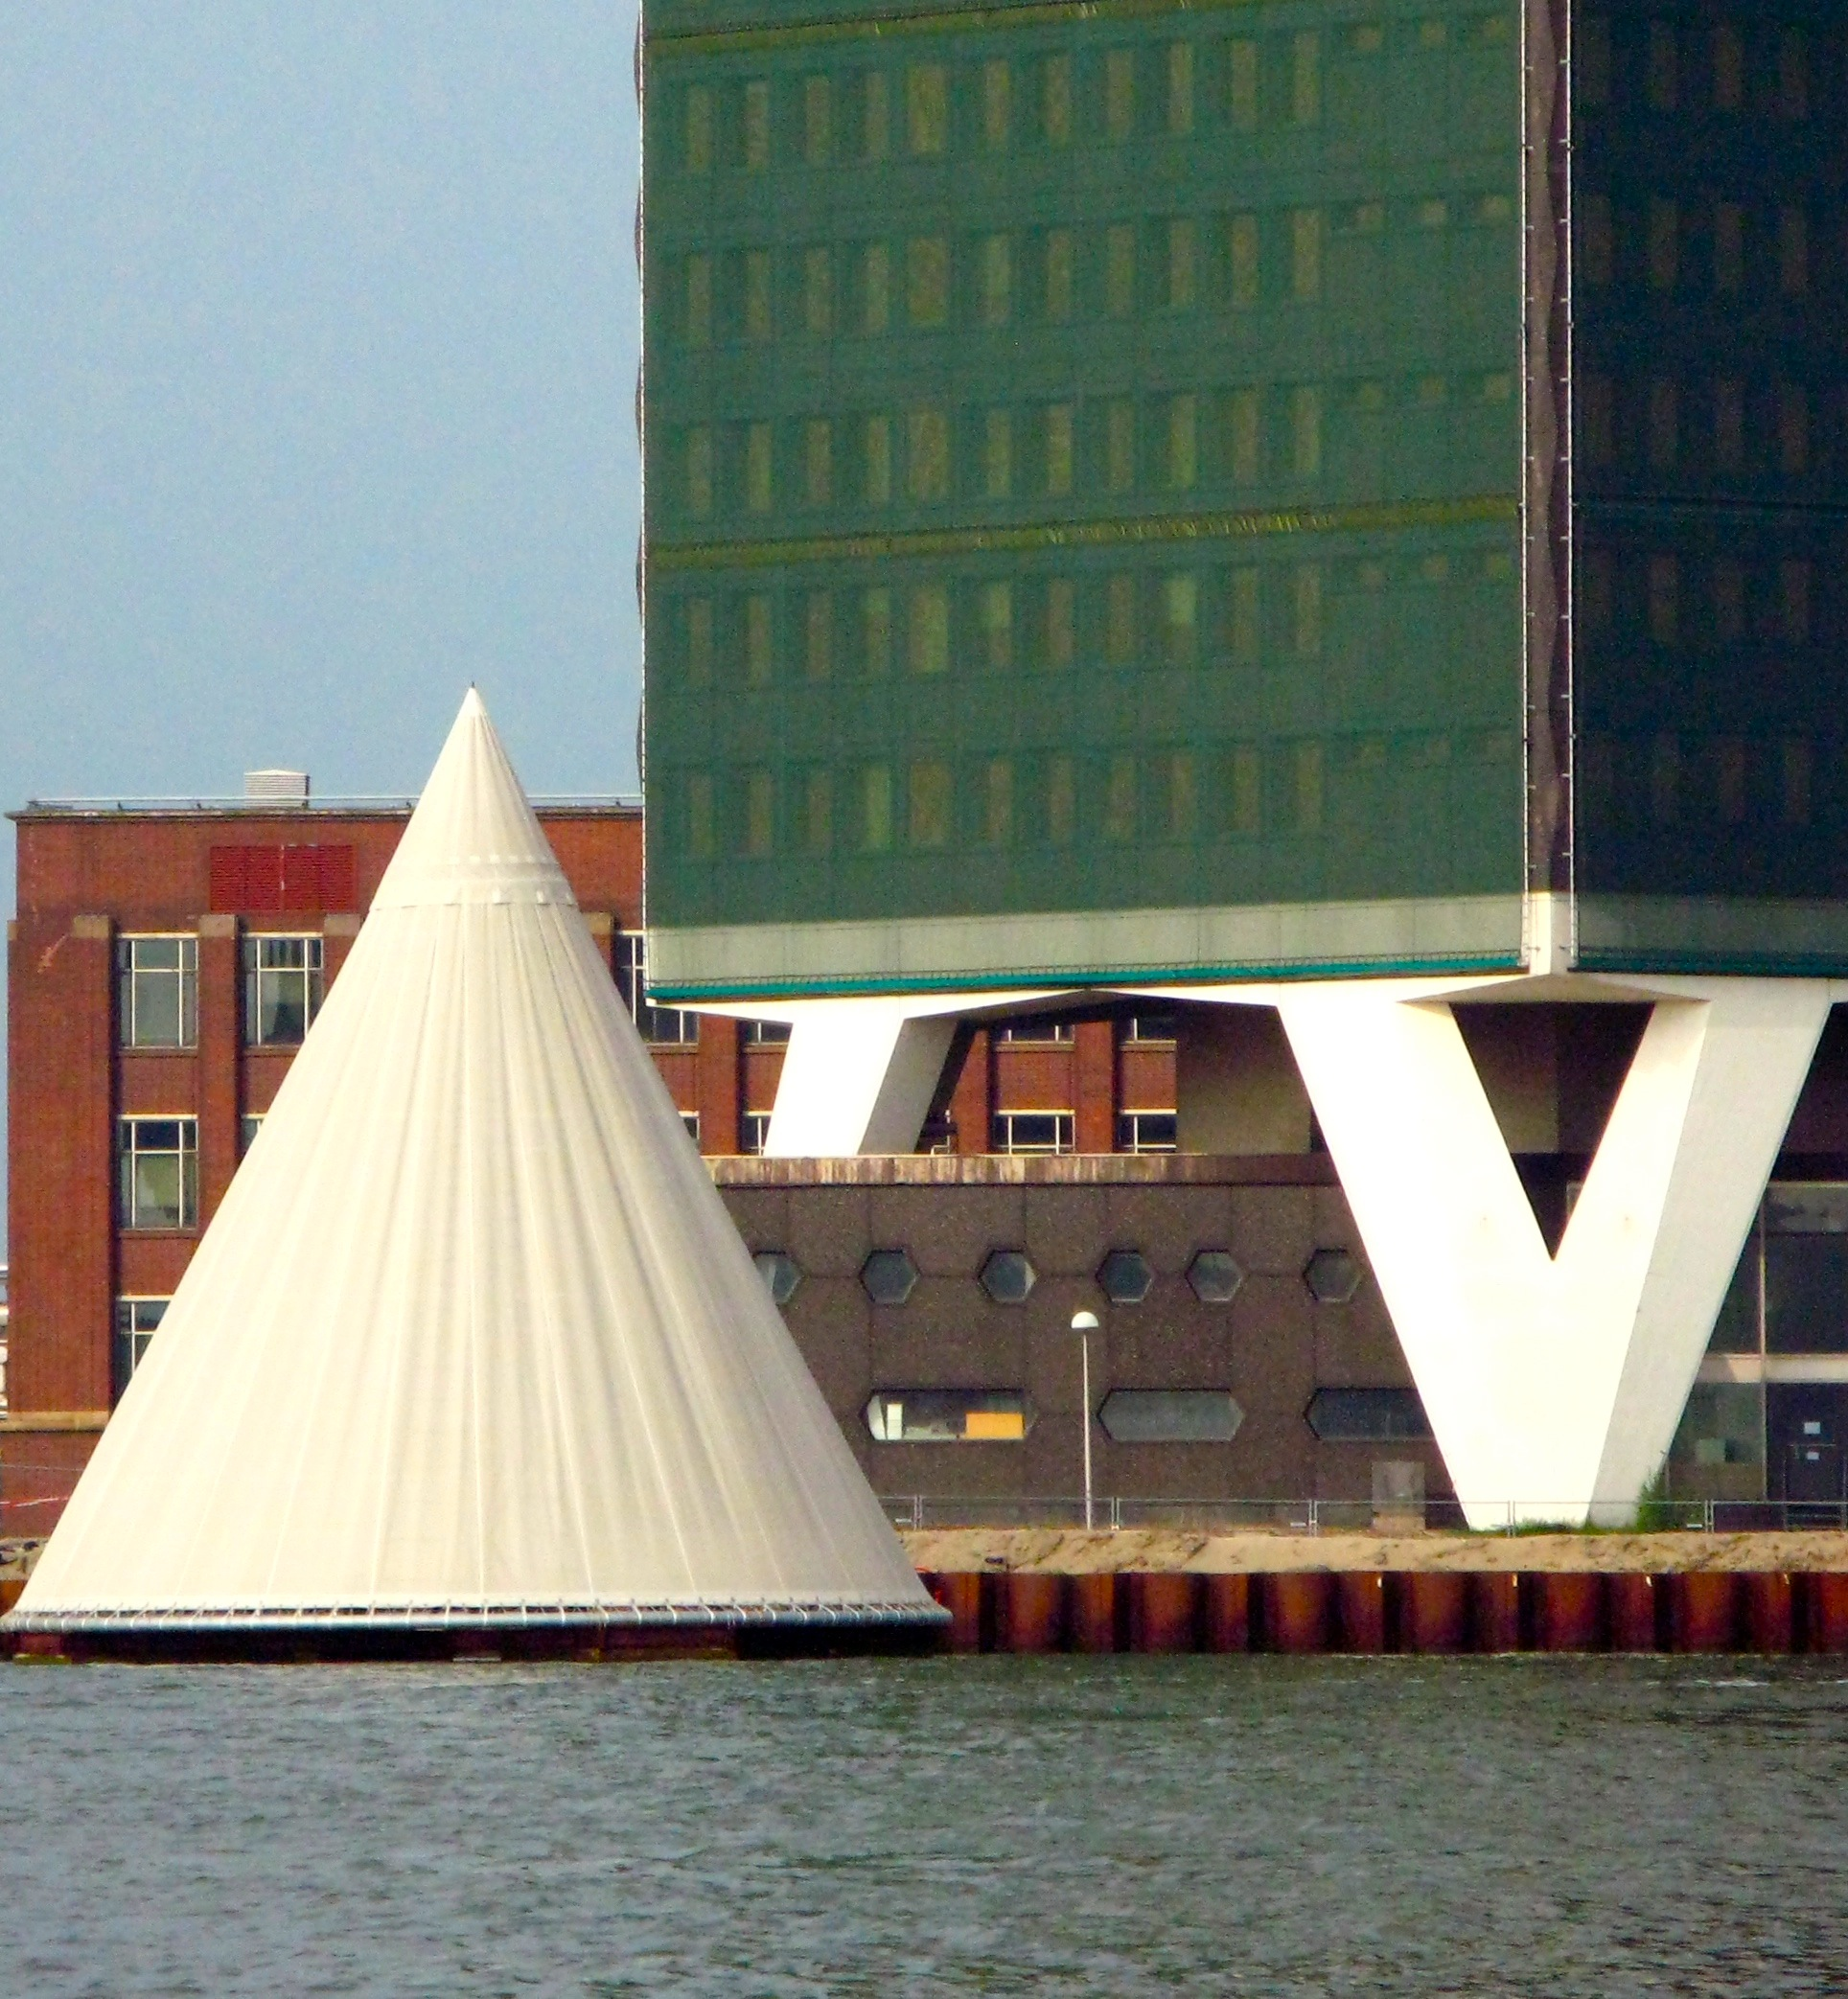
\includegraphics[width=0.95\textwidth]{\folder img/geometry_lesson.jpg}
  \begin{center}
    {\large ``Geometry lesson''}\par
    Foto di kevindooley\par
    \url{http://www.flickr.com/photos/pagedooley/2575606606/}\par
    Licenza: Creative Commons Attribution\par
  \end{center}
\newpage

\section{Introduzione alla geometria 
razionale}\label{sect:intro_geometria_razionale}
\subsection{Breve nota storica}
La parola geometria deriva dal greco antico: \textgreek{gewmetr'ia}, 
composta da \textgreek{gew} (geo) che significa ``terra'' e da 
\textgreek{metr'ia} (metria) che significa ``misura'', tradotto alla 
lettera significa ``misura della terra''. Secondo una tradizione 
storica, durante il VI secolo \aC{} alcuni matematici e pensatori 
greci (principalmente Talete e Pitagora) cominciarono a organizzare 
in maniera razionale (secondo il susseguirsi di ragionamenti logici) 
le conoscenze geometriche che egiziani e babilonesi avevano raggiunto 
nei secoli precedenti. Lo storico greco Erodoto, vissuto tra il 484 
\aC{} e il 425 \aC, racconta che a causa delle periodiche inondazioni 
del fiume Nilo gli egiziani erano costretti a ricostruire ogni anno i 
confini dei singoli possedimenti terrieri e in questo modo avevano 
sviluppato delle modalità tecniche per la misura della terra 
(\textgreek{gewmetr'ia} appunto).

Ritrovamenti più recenti di tavolette di creta del periodo babilonese 
incise con caratteri cuneiformi ci fanno ritenere che la cultura 
babilonese possedesse già delle sofisticate conoscenze geometriche. 
Di certo sappiamo che nel III secolo \aC{} il matematico ellenico 
Euclide\footnote{vissuto molto probabilmente durante il regno di 
Tolomeo I (367 \aC{} ca. - 283 \aC).}, direttore della grande 
biblioteca di Alessandria in Egitto, diede una struttura razionale 
alle conoscenze geometriche note sino ad allora scrivendo una delle 
più grandi opere della cultura occidentale, gli \emph{Elementi} (in 
greco \textgreek{Stoiqeia}). Questa grande opera è organizzata in 13 
libri, di cui i primi sei riguardano la Geometria Piana, i successivi 
quattro trattano i rapporti tra grandezze e gli ultimi tre riguardano 
la Geometria Solida. Essa prese il posto di tutti i libri precedenti 
sulla geometria e servì come testo fondamentale nell'antichità e nel 
medioevo; è stata usata come libro scolastico di geometria fino ai 
nostri giorni. La sua considerazione presso i Romani fu modesta, ma 
fu grandissima presso i Bizantini e gli Arabi. Proprio questi ultimi 
la reintrodussero in Europa dopo la perdita medievale, grazie alla 
traduzione di Adelardo di Bath\footnote{traduttore, filosofo e 
matematico britannico (1080 - 1152).} (secolo XII).

Dal punto di vista della struttura logica, gli \emph{Elementi} di 
Euclide sono organizzati a partire da cinque assiomi (nozioni comuni 
evidenti), cinque postulati (proposizioni che si richiede siano 
assunte come vere, senza dimostrazione) e 23 definizioni. L'opera di 
Euclide è rimasta nella nostra cultura l'unico punto di riferimento 
per lo studio della geometria, fino a quando, contestualmente allo 
studio dei fondamenti delle altre branche della matematica, i 
matematici cercarono di dare una base più rigorosa alla geometria di 
Euclide. Un'impostazione assiomatica più moderna venne data dal 
matematico tedesco David Hilbert\footnote{(1862 - 1943).} nel libro 
\emph{Grundlagen der Geometrie} (Fondamenti della geometria) 
pubblicato nel 1899, nel quale la geometria veniva fondata su ben 21 
assiomi.

\subsection{Lo spazio fisico e la geometria}
La geometria nasce come studio sistematico dello spazio fisico e 
delle forme che in esso si muovono. Lo spazio in cui ci muoviamo è per 
tutti una delle prime esperienze che facciamo fin dai primi mesi di 
vita. I nostri sensi determinano le sensazioni che ci permettono di 
riconoscere le forme degli oggetti e i loro movimenti. Tuttavia, le 
nozioni geometriche come quelle di punto, retta, rettangolo, cubo, 
sfera \ldots non trovano un perfetto riscontro nella realtà fisica. 
Nello spazio fisico non esistono, infatti, punti e rette come li 
descrive la geometria, né figure a due sole dimensioni, né cubi o 
sfere perfette. La geometria si propone quindi di fornire un 
``modello'' ideale della realtà fisica, sia per le forme degli 
oggetti sia per le proprietà dello spazio. 

Fino alla seconda metà dell'Ottocento, matematici e filosofi sono 
stati sostanzialmente d'accordo nel considerare la geometria come la 
scienza che descriveva razionalmente le proprietà dello spazio 
fisico. Galileo Galilei\footnote{fisico, filosofo, astronomo e 
matematico italiano (1564 - 1642).} ne \emph{Il saggiatore} (1623) 
scriveva:
\begin{quoting}
La filosofia è scritta in questo grandissimo libro che continuamente 
ci sta aperto innanzi a gli occhi (io dico l'universo), ma non si può 
intendere se prima non s'impara a intender la lingua, e conoscer i 
caratteri, ne' quali è scritto. Egli è scritto in lingua matematica, 
e i caratteri son triangoli, cerchi, ed altre figure geometriche, 
senza i quali mezi è impossibile a intenderne umanamente parola; 
senza questi è un aggirarsi vanamente per un oscuro laberinto.
\end{quoting}
A partire dalla seconda metà del XIX secolo, i matematici si sono 
invece convinti che la geometria non descrive esattamente lo spazio 
fisico, che sono possibili più geometrie ugualmente vere dal punto di 
vista logico e matematico. Lo studio matematico della geometria si è 
allora differenziato dallo studio dello spazio fisico e da quello 
dello spazio psicologico percepito dall'uomo con i suoi sensi. I 
matematici hanno accettato l'esistenza di diverse geometrie 
matematicamente possibili, si sono accontentati di costruire dei 
modelli astratti e hanno lasciato ai fisici la ``scelta'' del modello 
che meglio si adatta a descrivere i fenomeni fisici 
dall'infinitamente piccolo all'infinitamente grande. La geometria 
allora è diventata una branca della matematica alla quale i matematici 
hanno cercato di dare un fondamento esclusivamente logico, 
indipendente dalle esperienze fisiche. 

Il legame tra fisica e matematica non si è mai rotto. Con il passare 
dei secoli, ci si è resi sempre più conto di quanto la ``geometria'' 
del mondo fisico sia molto complessa e di come alcune nuove geometrie 
riescono a descrivere meglio fenomeni che con la vecchia geometria di 
Euclide non si riusciva a spiegare.

\section{Il metodo assiomatico, i concetti primitivi e le 
definizioni}\label{sect:metodo_assiomatico_concetti_primitivi}
La geometria, sin dai tempi di Euclide, è stata organizzata 
assiomaticamente, partendo cioè dalle fondamenta. Nella matematica 
queste fondamenta sono costituite dai concetti primitivi e dagli 
assiomi. Gli \emph{enti primitivi} sono le nozioni che si decide di 
non definire. Ci si può rendere facilmente conto, infatti, che non 
tutto può essere definito, poiché in ogni nozione che si definisce si 
deve fare ricorso ad altre nozioni, le quali a loro volta devono 
essere definite per mezzo di altre nozioni e così via all'indietro 
senza che teoricamente questo processo abbia mai una fine, arrivando 
necessariamente ad alcune nozioni così primitive da non poter essere 
definite con altre nozioni più elementari. A queste nozioni non è né 
necessario né possibile associare alcun significato esplicito; è 
invece fondamentale esprimere le loro proprietà esclusivamente 
attraverso \emph{assiomi}, cioè attraverso proprietà non dimostrabili 
che indicano però come gli enti primitivi devono e possono essere 
usati. Il matematico Hilbert utilizza tre enti primitivi -- punto, 
linea e piano -- e 21 assiomi. A partire dagli enti primitivi si 
fanno derivare tutte le \emph{definizioni} degli enti geometrici.

\subsection{Nozioni di logica}

Assumiamo come ``primitivo'' il concetto base di proposizione (o 
``giudizio'' secondo la terminologia del grande filosofo greco 
Aristotele\footnote{(384 o 383 \aC{} - 322 \aC).}): chiamiamo 
\emph{proposizione} una frase (affermativa o negativa) a cui abbia 
senso associare un valore di verità, sia esso \emph{vero} (V) oppure 
\emph{falso} (F).

Per esempio, sono proposizioni logiche affermazioni del tipo <<Una 
retta ha infiniti punti>>, <<\(2+3=10\)>>. Non sono proposizioni 
logiche le frasi <<\np{1000} è un numero grande>>, <<il quadrato è 
semplice>>. Mentre la prima frase esprime un'affermazione vera e la 
seconda un'affermazione falsa, la terza e la quarta esprimono 
affermazioni non valutabili oggettivamente pertanto di queste ultime 
non si può dire se sono vere o false.

La logica delle proposizioni si fonda sui seguenti tre principi della 
logica aristotelica:
\begin{itemize*}
\item il \emph{principio di identità}: ogni oggetto è identico a se 
stesso e a nessun altro oggetto;
\item il \emph{principio di non contraddizione}: una stessa 
proposizione non può essere contemporaneamente vera e falsa;
\item il \emph{principio del terzo escluso}: una proposizione può 
essere solo vera o falsa, non può assumere un diverso valore di 
verità.
\end{itemize*}

Il corpo della geometria, come di qualunque altra teoria matematica, 
è costituito da \emph{proposizioni}, cioè da affermazioni che 
riguardano gli enti geometrici e che sono vere o false. Le 
proposizioni possono essere semplici affermazioni (\emph{proposizioni 
atomiche}) oppure possono essere ottenute da una o più proposizioni 
elementari legate tra di loro attraverso connettivi logici (elementi 
linguistici del tipo ``non'', ``e'', ``oppure'', ``o \ldots{} o'', 
``quindi'', ``se \ldots{} allora'', ``se e solo se''). In questo caso 
si parla di \emph{proposizioni composte} o molecolari
Per esempio, la proposizione <<un triangolo ha tre lati e ha tre 
angoli>> è composta dalle proposizioni <<un triangolo ha tre lati>> e 
<<un triangolo ha tre angoli>> unite dal connettivo ``e''.

\paragraph{La congiunzione} di due proposizioni si ottiene con il 
connettivo ``e'' (\emph{et}, \emph{and}, \(\wedge\)): la proposizione 
\(r\) ottenuta dalla congiunzione delle proposizioni \(p\) e \(q\), in 
simboli può essere scritta come
\[\boxed{ % vedi naturali.tex riga 757
\vphantom{I}r=p\wedge q}\]
ed è vera se entrambe le proposizioni \(p\) e \(q\) sono contestualmente 
vere, mentre è falsa quando anche una sola delle due proposizioni è 
falsa.
Per esempio, <<ho avuto 7 in italiano e matematica>> è 
un'affermazione vera solo quando ho avuto 7 in entrambe le materie e 
falsa in tutti gli altri casi.

Per esprimere in maniera sintetica tutte le possibilità del valore di 
verità di una proposizione composta, si usa una tabella a doppia 
entrata, detta \emph{tavola di verità}, che per la congiunzione 
logica è la seguente
\begin{center}
 \begin{tabular*}{.25 \textwidth}{@{\extracolsep{\fill}}*{3}{c}}
 \toprule
~\(p\) &~\(q\) &~\(p\wedge q\)\\
\midrule
~V & V & V \\
~V & F & F \\
~F & V & F \\
~F & F & F \\
\bottomrule
 \end{tabular*}
\end{center}

\paragraph{La disgiunzione (inclusiva)} di due proposizioni si 
ottiene con il connettivo ``o'' (\emph{vel}, \emph{or}, \({\vee}\)): la 
proposizione \(s\) ottenuta dalla disgiunzione di due proposizioni \(p\) 
e \(q\), in simboli
}\]\vphantom{I}s=p\vee q}\]
è vera quando almeno una delle due proposizioni è vera ed è falsa 
solo se entrambe le proposizioni sono false.
\begin{center}
 \begin{tabular*}{.25 \textwidth}{@{\extracolsep{\fill}}*{3}{c}}
 \toprule
~\(p\) &~\(q\) &~\(p\vee q\)\\
\midrule
~V & V & V \\
~V & F & V \\
~F & V & V \\
~F & F & F \\
\bottomrule
 \end{tabular*}
\end{center}

\paragraph{La negazione} di una proposizione si ottiene con il 
connettivo ``non'' (\emph{non}, \emph{not}, \(\neg\)), un operatore 
che, a differenza dei precedenti, non lega più proposizioni ma agisce 
su un'unica proposizione (per questo si dice che è un operatore 
unario, in analogia all'operazione insiemistica di complementazione). 
La proposizione \(n\) data dalla negazione di una proposizione \(p\) si 
indica con il simbolo
}\]\vphantom{I}n=\neg p}\]
ed è vera se \(p\) è falsa, viceversa è falsa se \(p\) è vera.

La doppia negazione equivale ad un'affermazione, cioè \(\neg(\neg p)\) 
è equivalente a \(p\).
La tavola di verità è la seguente:
\begin{center}
 \begin{tabular*}{.25 \textwidth}{@{\extracolsep{\fill}}*{3}{c}}
 \toprule
~\(p\) &~\(\neg p\) &~\(\neg(\neg p)\)\\
\midrule
~V & F & V \\
~F & V & F \\
\bottomrule
 \end{tabular*}
\end{center}

\paragraph{La disgiunzione esclusiva} di due proposizioni si ottiene 
con il connettivo (o congiunzione) ``o \ldots{} o'' (\emph{aut}, 
\emph{xor}, \(\veebar\)): la proposizione \(t\) ottenuta dalla 
disgiunzione esclusiva di due proposizioni \(p\) e \(q\), in simboli
}\]\vphantom{I}t=p\veebar q}\]
è vera quando solo una delle due proposizioni è vera ed è falsa 
quando le due proposizioni sono entrambe vere o entrambe false.
Per esempio, nell'affermazione <<oggi il Milan vince o pareggia>> la 
congiunzione ``o'' ha valore esclusivo.

La disgiunzione esclusiva \(\veebar\) a volte non viene messa tra gli 
operatori logici fondamentali perché è esprimibile attraverso gli 
altri tre operatori presentati finora.
\begin{center}
 \begin{tabular*}{.25 \textwidth}{@{\extracolsep{\fill}}*{3}{c}}
 \toprule
~\(p\) &~\(q\) &~\(p\veebar q\)\\
\midrule
~V & V & F \\
~V & F & V \\
~F & V & V \\
~F & F & F \\
\bottomrule
 \end{tabular*}
\end{center}

\pagebreak
\begin{exrig}
\begin{esempio}
Date le seguenti proposizioni \(p=\)~<<un triangolo ha tre lati>> 
(Vera), \(q=\)~<<un triangolo ha tre vertici>> (Vera), \(r=\)~<<un 
triangolo ha quattro angoli>> (Falsa), \(s=\)~<<un triangolo ha tre 
dimensioni>> (Falsa), allora:
\begin{itemize*}
\item \(p\wedge q\) è vera,~~\(q\wedge r\) è falsa,~~\(r\wedge s\) è falsa;
\item \(p\vee q\) è vera,~~\(q\vee r\) è vera,~~\(r\vee s\) è falsa;
\item \(p\veebar q\) è falsa,~~\(q\veebar r\) è vera,~~\(r\veebar s\) è 
falsa.
\end{itemize*}
\end{esempio}
\end{exrig}

È piuttosto semplice capire il meccanismo della negazione se 
applicata a proposizioni atomiche, spesso è meno intuitivo il valore 
di verità della negazione di una proposizione più complessa.
Ad esempio, la negazione di \(p\wedge q\) non è \(\neg p\wedge \neg q\) 
bensì \(\neg p\vee \neg q\), mentre la negazione di \(p\vee q\) è \(\neg 
p\wedge \neg q\) e non \(\neg p\vee \neg q\).
In formule:
}\]\vphantom{I}\neg (p\wedge q)= (\neg p)\vee (\neg 
q)\qquad\text{e}\qquad\neg (p\vee q)= (\neg p)\wedge (\neg q).}\]

Per esempio, <<non è vero che Marco e Luca sono stati bocciati>> può 
voler dire che entrambi non sono stati bocciati o solo uno di loro 
non è stato bocciato.

Queste uguaglianze prendono il nome di \emph{leggi di De 
Morgan}\footnote{dal nome del matematico e logico britannico 
Augustuts De Morgan (1806 - 1871).}, e la loro verifica può essere 
effettuata con la seguente tavola di verità:
\begin{center}
 \begin{tabular*}{.8 \textwidth}{@{\extracolsep{\fill}}*{8}{c}}
 \toprule
~\(p\) &~\(q\) &~\( \neg p \)&~\( \neg q \)&~\(p\wedge q\)&~\(\neg p\vee 
\neg 
q\)&~\(p\vee q\)&~\(\neg p\wedge \neg q\)\\
\midrule
~V & V & F & F & V & F & V & F \\
~V & F & F & V & F & V & V & F \\
~F & V & V & F & V & V & V & F \\
~F & F & V & V & F & V & F & V \\
\bottomrule
 \end{tabular*}
\end{center}

Come per le operazioni aritmetiche anche per gli operatori logici è 
possibile analizzarne le proprietà. Ne indichiamo qualcuna a titolo 
di esempio:
\begin{itemize*}
\item \((p\wedge q)\wedge r= p\wedge (q\wedge r)\) proprietà 
\emph{associativa} della congiunzione;
\item \(p\wedge q= q\wedge p\) proprietà \emph{commutativa} della 
congiunzione;
\item \(p\wedge (q\vee r)= (p\wedge q)\vee (p\wedge r)\) proprietà 
\emph{distributiva} della congiunzione rispetto alla disgiunzione.
\end{itemize*}

Una proposizione che è sempre vera indipendentemente dalla verità 
degli elementi che lo compongono è detta \emph{tautologia}. Una 
proposizione che è sempre falsa indipendentemente dalla verità dei 
suoi elementi è invece detta \emph{contraddizione}.

Per esempio, la proposizione composta \(p\wedge \neg p\) è una 
contraddizione in quanto è sempre falsa, mentre la proposizione 
composta \(p\vee \neg p\) è una tautologia poiché è sempre vera.

\vspazio\ovalbox{\risolvii \ref{ese:1.1}, \ref{ese:1.2}, 
\ref{ese:1.3}, \ref{ese:1.4}, \ref{ese:1.5}, \ref{ese:1.6}, 
\ref{ese:1.7}, \ref{ese:1.8}, \ref{ese:1.9}, \ref{ese:1.10}, 
\ref{ese:1.11}}

\subsection{Predicati e quantificatori}

Una proposizione che fa riferimento a una proprietà o caratteristica 
di alcuni elementi di un insieme si chiama \emph{predicato} (o 
\emph{enunciato}). Le frasi formate da un predicato che ha alcuni 
argomenti incogniti si dicono \emph{enunciati aperti}.
Per esempio, \(p=\)~<<\(x\) è un numero intero maggiore di 10>> è un 
enunciato aperto.

Consideriamo ora le seguenti affermazioni:
\begin{itemize*}
\item <<tutti gli uomini sono mortali>> si riferisce a un qualsiasi 
essere umano;
\item <<tutti i multipli di 6 sono anche multipli di 2>> è vera per 
tutti i numeri multipli di 6;
\item <<ogni numero negativo è minore di ogni numero positivo>>.
\end{itemize*}
I predicati precedenti non riguardano un elemento specifico ma una 
certa quantità di elementi. I termini ``tutti'' e ``ogni'', detti 
\emph{quantificatori universali}, indicano che una proprietà è vera 
per tutti gli elementi di un certo insieme. In logica matematica per 
indicare il quantificatore universale si usa il simbolo \(\forall\), 
che si legge ``per ogni''.

Vediamo ora i seguenti predicati:
\begin{itemize*}
\item <<esiste un numero che elevato al quadrato dà \(16\)>>;
\item <<alcuni numeri pari sono anche multipli di \(3\)>>.
\end{itemize*}
Queste affermazioni esprimono proprietà che sono vere almeno per un 
elemento dell'insieme di riferimento: la prima frase è vera per i 
numeri \(+4\) e \(-4\), la seconda frase è vera per i numeri \(6\), \(12\), 
\(18\), \ldots{}
I termini ``c'è almeno'', ``alcuni'', ``esiste almeno uno'' si dicono 
\emph{quantificatori esistenziali} ed in logica matematica si 
indicano con il simbolo \(\exists\), che si legge ``esiste''.

Bisogna prestare particolare attenzione quando si negano frasi in cui 
compaiono i quantificatori. Per esempio la negazione di <<tutti i 
gatti fanno le fusa>> non è <<nessun gatto fa le fusa>> bensì <<non 
tutti i gatti fanno le fusa>> che si può esprimere anche con il 
quantificatore esistenziale <<C'è almeno un gatto che non fa le 
fusa>>.
La negazione della frase <<l'anno scorso siamo stati tutti promossi>> 
non è <<l'anno scorso siamo stati tutti bocciati>> ma <<l'anno scorso 
non siamo stati tutti promossi>> ovvero <<l'anno scorso c'è stato 
almeno uno di noi che non è stato promosso>>.
La negazione della proposizione \(p=\)~<<tutti i quadrati hanno due 
diagonali>> è la proposizione \({\lnot}p=\)~<<non tutti i quadrati 
hanno due diagonali>>.
Il linguaggio comune ci potrebbe portare a considerare come negazione 
di \(p\) la proposizione <<nessun quadrato ha due diagonali>>, in 
realtà per avere la negazione della proposizione \(p\) basta che esista 
almeno un quadrato che non ha due diagonali.

\vspazio\ovalbox{\risolvii \ref{ese:1.12}, \ref{ese:1.13}, 
\ref{ese:1.14}}


\subsection{Implicazione}

Nel linguaggio matematico sono comuni proposizioni del tipo <<Se \(p\) 
allora \(q\)>>. Ad esempio <<se un numero è multiplo di \(12\) allora è 
multiplo di \(3\)>>. La frase precedente può essere espressa dicendo 
<<essere multiplo di \(12\) \emph{implica} essere multiplo di \(3\)>>.

In logica frasi del tipo <<se \(p\) allora \(q\)>> vengono tradotte 
utilizzando l'operatore \(\Rightarrow\) detto \emph{implicazione}.
La scrittura <<se \(p\) allora \(q\)>> si traduce quindi con la scrittura
}\]\vphantom{I}p\Rightarrow q}\]
che si legge ``\(p\) implica \(q\)''.

La proposizione \(p\) è detta \emph{antecedente}, (o \emph{ipotesi}) e 
la proposizione \(q\) è detta \emph{conseguente} (o \emph{tesi}).
Il significato logico della proposizione \(p\Rightarrow q\) è che 
<<tutte le volte che la proposizione \(p\) è vera allora risulta vera 
anche la proposizione \(q\)>>. Ovvero non si specifica il caso in cui 
\(p\) sia falsa.

Per esempio, l'affermazione <<se c'è il sole andiamo al mare>> è 
falsa solo quando c'è il sole e non andiamo al mare; l'affermazione, 
infatti, non dice nulla se il sole non c'è: quindi se non c'è il sole 
si è liberi di andare o non andare al mare. Anche l'affermazione <<se 
studi sarai promosso>> dice solo che se studi conseguirai la 
promozione, non dice nulla per il caso in cui tu non studi: in questo 
caso, infatti, potresti essere ugualmente promosso.

La tavola di verità è la seguente:
\begin{center}
 \begin{tabular*}{.25 \textwidth}{@{\extracolsep{\fill}}*{3}{c}}
 \toprule
~\(p\) &~\(q\) &~\(p\Rightarrow q\)\\
\midrule
~V & V & V \\
~V & F & F \\
~F & V & V \\
~F & F & V \\
\bottomrule
 \end{tabular*}
\end{center}

Uno degli errori logici più comuni è quello di pensare che da 
\(p\Rightarrow q\) si possa dedurre  \(\neg p\Rightarrow \neg q\).
Ad esempio dall'affermazione <<se piove prendo l'ombrello>> qualcuno 
può pensare che si possa dedurre <<se non piove non prendo 
l'ombrello>>. Riflettendoci, si intuisce che le due frasi non sono 
affatto consequenziali. Basta pensare che chi pronuncia la prima 
frase sta affermando che tutte le volte che piove prende naturalmente 
l'ombrello, ma non esclude la possibilità di prenderlo anche quando 
non piove (in effetti è saggio farlo se il cielo è coperto da 
nuvoloni neri!).

Così la frase (a) <<se \(x\) è multiplo di \(12\) allora è multiplo di 
\(3\)>> non vuol dire (b) <<se \(x\) non è multiplo di \(12\) allora non è 
multiplo di \(3\)>>.
Infatti la (a) è vera, mentre la (b) è falsa (si pensi ad esempio al 
numero \(6\) che non è multiplo di \(12\) ma è comunque multiplo di \(3\)).

Ciò che ragionevolmente si può dedurre da \(p\Rightarrow q\) è \(\neg 
q\Rightarrow \neg p\).
Ad esempio, da <<se \(x\) è multiplo di \(12\) allora è multiplo di \(3\)>> 
si può dedurre <<se \(x\) non è multiplo di \(3\) allora non è multiplo 
di \(12\)>>.

Data l'implicazione \(p\Rightarrow q\), la proposizione \(p\) viene detta 
\emph{condizione sufficiente} per \(q\). Mentre la proposizione \(q\) 
viene detta \emph{condizione necessaria} per \(p\).
Per esempio, <<studiare>> è condizione necessaria per <<essere 
promossi>> ma non è sufficiente.
Quest'ultima espressione fa appunto riferimento al fatto che da 
\(p\Rightarrow q\) si può dedurre  \(\neg q\Rightarrow \neg p\). Ossia 
\(q\) è necessaria per \(p\) in quanto se non è vera \(q\) non è vera 
neanche \(p\).

Calcoliamo la tavola di verità di \(p\Rightarrow q\) e di \(\neg 
q\Rightarrow \neg p\) 
\begin{center}
 \begin{tabular*}{.6 \textwidth}{@{\extracolsep{\fill}}*{6}{c}}
 \toprule
~\(p\) &~\(q\) &~\(p\Rightarrow q\) &~\( \neg q \) &~\( \neg p \)&~\( \neg 
q\Rightarrow \neg p \) \\
\midrule
~V & V & V & F & F & V\\
~V & F & F & V & F & F\\
~F & V & V & F & V & V\\
~F & F & V & V & V & V\\
\bottomrule
 \end{tabular*}
\end{center}
Come si vede, le due proposizioni hanno gli stessi valori di verità.

In generale, data un'implicazione \(p\Rightarrow q\) 
(\emph{proposizione diretta}):
\begin{itemize*}
\item l'implicazione \(\neg p\Rightarrow \neg q\) si dice 
\emph{contraria} di \(p\Rightarrow q\);
\item l'implicazione \(q\Rightarrow p\) si dice \emph{inversa} di 
\(p\Rightarrow q\);
\item l'implicazione \(\neg q\Rightarrow \neg p\) si dice 
\emph{contronominale} (o \emph{controinversa}) di \(p\Rightarrow q\).
\end{itemize*}

\paragraph{La doppia implicazione} o \emph{equivalenza logica} di due 
proposizioni \(p\) e \(q\) dà luogo a una proposizione che in simboli si 
rappresenta con
}\]\vphantom{I}p\Leftrightarrow q}\]
(leggasi ``\(p\) se e solo se \(q\)'') che è vera solo se \(p\) e \(q\) sono 
entrambe vere o entrambe false. La tavola di verità è la seguente:
\begin{center}
 \begin{tabular*}{.75 \textwidth}{@{\extracolsep{\fill}}*{6}{c}}
 \toprule
~\(p\) &~\(q\) &~\(p\Leftrightarrow q\) &~\( p\Rightarrow q \) &~\( 
q\Rightarrow p \)&~\( (p\Rightarrow q)\wedge (q\Rightarrow p) \) \\
\midrule
~V & V & V & V & V & V\\
~V & F & F & F & V & F\\
~F & V & F & V & F & F\\
~F & F & V & V & V & V\\
\bottomrule
 \end{tabular*}
\end{center}
L'operatore \(\Leftrightarrow \) è detto \emph{doppia implicazione} 
perché se vale \(p\Leftrightarrow q\) allora valgono sia \(p\Rightarrow 
q\) che \(q\Rightarrow p\) (e viceversa). Nella tabella precedente, 
infatti, è stata messa in evidenza l'equivalenza logica tra la 
proposizione \(p\Leftrightarrow q\) e la proposizione \((p\Rightarrow 
q)\wedge (q\Rightarrow p)\).

L'equivalenza logica è un relazione di equivalenza, infatti verifica 
le seguenti proprietà:
\begin{itemize*}
\item \(p\Leftrightarrow p\): è \emph{riflessiva};
\item se \(p\Leftrightarrow q\) allora vale anche \(q\Leftrightarrow p\): 
è \emph{simmetrica};
\item se \(p\Leftrightarrow q\) e \(q\Leftrightarrow r\) allora vale 
anche \(p\Leftrightarrow r\): è \emph{transitiva}.
\end{itemize*}

In matematica si usa spesso l'espressione <<\(p\) è \emph{condizione 
necessaria e sufficiente} per \(q\)>>. Per esempio <<condizione 
necessaria e sufficiente affinché un numero sia divisibile per \(3\) è 
che la somma delle sue cifre sia divisibile per \(3\)>>. Il significato 
della frase è che <<\(p\) è sufficiente per \(q\)>> e inoltre <<\(p\) è 
necessario per \(q\)>>. In altre parole significa che  \(p\Rightarrow q\) 
e \(q\Rightarrow p\). Nel caso dell'esempio vale quindi sia 
l'implicazione diretta, <<se un numero è divisibile per \(3\) allora la 
somma delle sue cifre è divisibile per \(3\)>>, che quella inversa, 
<<se la somma delle cifre di un numero è divisibile per \(3\) allora il 
numero stesso è divisibile per \(3\)>>.

\vspazio\ovalbox{\risolvii \ref{ese:1.15}, \ref{ese:1.16}, 
\ref{ese:1.17}}

\subsection{I teoremi}

Un \emph{teorema} è una proposizione composta del tipo  \(I\Rightarrow 
T\), cioè una implicazione tra due proposizioni, dette \emph{ipotesi} 
(\(I\)) e \emph{tesi} (\(T\)).

Dimostrare un teorema significa fare un ragionamento logico che 
permetta di concludere che la tesi è vera avendo supposto che 
l'ipotesi sia vera. Nel caso in cui un teorema sia dimostrabile 
all'interno di una teoria, si dice che è un teorema valido.

In riferimento alla terminologia usata quando abbiamo parlato 
dell'implicazione, chiamiamo  \(I\Rightarrow T\) \emph{teorema 
diretto}, \(T\Rightarrow I\) \emph{teorema inverso}, \(\neg I\Rightarrow 
\neg T\) \emph{teorema contrario} e \(\neg T\Rightarrow \neg I\) 
\emph{teorema controinverso}. Ribadiamo l'equivalenza tra il teorema 
diretto ed il teorema controinverso, nonché l'equivalenza tra il 
teorema contrario ed il teorema inverso, mentre in generale la 
validità del teorema diretto non implica la validità del teorema 
inverso, e viceversa.

Nel caso particolare in cui vale sia \(I\Rightarrow T\) che 
\(T\Rightarrow I\), si scrive  \(I\Leftrightarrow T\) e si dice che 
ipotesi e tesi sono \emph{logicamente equivalenti}. Più precisamente, 
nel linguaggio specifico delle scienze che fanno uso della logica, e 
quindi anche nel linguaggio della Geometria Razionale, se vale 
\(I\Rightarrow T\), si dice che <<\(I\) è condizione sufficiente per 
\(T\)>> e anche che <<\(T\) è condizione necessaria per \(I\)>>; se in 
particolare vale  \(I\Leftrightarrow T\), si usa dire che <<\(I\) è 
condizione necessaria e sufficiente per \(T\)>>.

In generale incontreremo molti teoremi che vengono denominati 
genericamente \emph{proposizioni}, perché il nome di ``teorema'' 
viene tradizionalmente attribuito solo ai teoremi più importanti. 
Inoltre si usa chiamare \emph{lemma} una proposizione che non ha una 
grande importanza di per sé, ma che è particolarmente utile per la 
dimostrazione di altri teoremi. Si chiama invece \emph{corollario} un 
teorema importante che è una conseguenza immediata di un altro 
teorema.

Così come abbiamo visto che non è possibile definire tutto e che 
quindi bisogna assumere alcune nozioni come primitive, analogamente 
non è possibile dimostrare tutte le proposizioni di una teoria. 
Alcune proposizioni devono essere assunte come vere e costituiscono la 
base della dimostrazione dei teoremi; queste proposizioni si chiamano 
\emph{postulati} o \emph{assiomi}. Risulta evidente che cambiando sia 
pure uno solo degli assiomi cambiano anche i teoremi dimostrabili e 
quindi la teoria.

In generale, come abbiamo detto, dato un teorema (diretto) del tipo 
\(p\Rightarrow q\), la sua validità non garantisce la validità del 
teorema inverso \(q\Rightarrow p\). Questo però può succedere. In ogni 
caso, se sono vere \(p\Rightarrow q\) e \(q\Rightarrow p\), le due 
proposizioni sono \emph{logicamente equivalenti}, ossia 
\(p\Leftrightarrow q\).
\begin{exrig}
\begin{esempio}
Teorema: <<un triangolo che ha i lati uguali ha anche gli angoli 
uguali>>.
\begin{itemize}
\item Il teorema si può schematizzare nel seguente modo: \(p=\)~<<un 
triangolo ha i lati uguali>>; \(q=\)~<<un triangolo ha gli angoli 
uguali>>. Il teorema enunciato è \(p\Rightarrow q\).
\item  Il teorema inverso è  \(q\Rightarrow p\), cioè <<un triangolo 
che ha gli angoli uguali ha anche i lati uguali>>.
\end{itemize}
In tale esempio sono validi sia il teorema diretto che quello 
inverso. Il fatto che uno dei due teoremi sia chiamato diretto e 
l'altro inverso è un fatto soggettivo, che può dipendere 
semplicemente dall'ordine con cui si enunciano i teoremi.
Il teorema precedente si può esporre allora nel seguente modo:
\item Teorema: <<un triangolo ha i lati uguali se e solo se ha gli 
angoli uguali>>.
\end{esempio}
\end{exrig}

\subsection{La deduzione}

Nel paragrafo precedente abbiamo parlato in modo generico di 
implicazione, deduzione, dimostrazione. Facciamo ora un po' di 
chiarezza sull'uso di questi termini. L'\emph{implicazione} è 
un'operazione tra proposizioni, mentre la \emph{deduzione} è il 
ragionamento logico che costituisce la base della dimostrazione di un 
teorema. Per l'implicazione materiale si usa il simbolo \(\rightarrow\) 
mentre per la deduzione logica si usa il simbolo \(\Rightarrow\).

La frase <<se 5 è un numero pari, allora il triangolo ha 4 lati>> è 
perfettamente valida dal punto di vista logico ed anzi è vera, poiché 
la premessa (proposizione antecedente) è falsa, per cui 
l'implicazione è vera anche se la proposizione conseguente è falsa (si 
tenga presente la tavola di verità di \(p\Rightarrow q\)).
Si noti però che la definizione di implicazione ha senso solamente se 
la premessa è vera, il suo ampliamento al caso in cui la premessa è 
falsa è motivata da ragioni di completezza della trattazione. Bisogna 
quindi fare attenzione ad usare l'implicazione logica quando la 
premessa è falsa. Teniamo comunque conto che se \(p\) è falsa allora 
\((p\Rightarrow q)\wedge(p\Rightarrow \neg q)\) cioè \(p\Rightarrow 
(q\wedge \neg q)\) è vera. Ma  \(q\wedge \neg q\) è una contraddizione, 
quindi una premessa falsa implica sempre una contraddizione.

In realtà, la \emph{dimostrazione} di un teorema non è la verifica 
della validità dell'implicazione, anzi è un procedimento che fa uso 
della validità dell'implicazione stessa. In un teorema si parte dal 
supporre vera l'ipotesi e si dimostra, mediante un ragionamento 
logico che si basa sugli assiomi e su altri teoremi già dimostrati in 
precedenza, che anche la tesi è vera (questo se si segue il 
\emph{procedimento diretto}). Se si segue invece il 
\emph{procedimento indiretto} (o \emph{per assurdo}), si suppone che 
la tesi sia falsa e, sempre mediante ragionamento logico basato su 
assiomi e altri teoremi già dimostrati, si arriva ad affermare che 
l'ipotesi è falsa (cosa che non si deve accettare).

Le principali regole del corretto ragionamento seguono alcuni schemi 
particolari (detti \emph{sillogismi}, dal nome attribuito ad essi da 
Aristotele). Presentiamo qui i quattro principali sillogismi: il 
\emph{modus ponens}, il \emph{modus tollens}, il \emph{sillogismo 
disgiuntivo} e il \emph{sillogismo ipotetico}.
\begin{center}
 \begin{tabular*}{.8 \textwidth}{@{\extracolsep{\fill}}*{6}{c}}
 \toprule
 &Modus&Modus&\multicolumn{2}{c}{Sillogismo}&Sillogismo\\
 &ponens&tollens&\multicolumn{2}{c}{disgiuntivo}&ipotetico\\
\midrule
1\textsuperscript{a} premessa & \(p\Rightarrow q\) & \(p\Rightarrow q\) & 
\(p\vee q\) & \(p\vee q\) & \(p\Rightarrow q\)\\
2\textsuperscript{a} premessa & \( p \) & \( \neg q \) & \( \neg p \) & \( 
\neg q \)  & \(q\Rightarrow r\)\\
\midrule
conclusione & \( q \) & \( \neg p \) & \( q \) & \( p \) & \(p\Rightarrow r\)\\
\bottomrule
 \end{tabular*}
\end{center}
Suggeriamo una lettura degli schemi appena esposti:
\begin{itemize*}
\item \emph{modus ponens}: se sappiamo che \(p\) implica \(q\) e che \(p\) 
è vera, allora possiamo concludere che anche \(q\) è vera (metodo 
diretto di dimostrazione);
\item \emph{modus tollens}: se sappiamo che \(p\) implica \(q\) e che \(q\) 
è falsa, allora possiamo concludere che anche \(p\) è falsa (metodo 
indiretto di dimostrazione);
\item \emph{sillogismo disgiuntivo}: se sappiamo che, tra \(p\) e \(q\), 
almeno una delle due è vera, e sappiamo che \(p\) (rispettivamente \(q\)) 
è falsa, allora possiamo concludere che \(q\) (rispettivamente \(p\)) è 
vera;
\item \emph{sillogismo ipotetico}: se sappiamo che \(p\) implica \(q\) e 
che \(q\) implica \(r\), allora possiamo concludere che \(p\) implica \(r\) 
(proprietà transitiva dell'implicazione).
\end{itemize*}

Altre regole (note come i \emph{giudizi} di Aristotele) fanno uso dei 
predicati e dei quantificatori. Riprendiamo un esempio precedente 
traducendo la frase <<tutti i quadrati hanno due diagonali>> e la sua 
negazione <<non tutti i quadrati hanno due diagonali>> in formule che 
fanno uso anche del linguaggio degli insiemi. Se chiamiamo \(Q\) 
l'insieme di tutti i quadrati e \(P\) la proprietà dell'avere due 
diagonali, se \(x\) è il generico quadrato (elemento di \(Q\)), \(P(x)\) è 
il predicato <<\(x\) gode della proprietà \(P\)>>, cioè <<\(x\) ha due 
diagonali>>, la frase <<tutti i quadrati hanno due diagonali>> si 
traduce in simboli: \({\forall}x\in Q\), \(P(x)\).

La sua negazione è: <<esiste almeno un quadrato che non ha due 
diagonali>>, cioè che non gode della proprietà \(P\), e si traduce in 
simboli così: \(\exists x\in Q\), \(\neg P(x)\).
In quest'ultimo caso, la virgola può anche essere sostituita da una 
barra verticale ``\textbar'' o da ``:'' e si legge ``tale che''.

Analogamente, una frase del tipo <<esiste almeno un numero naturale 
che sia divisore di \(10\)>> può scriversi come: \(\exists n\in\N\mid 
D(n)\), dove \(D\) è la proprietà dell'essere divisore di \(10\) e \(D(n)\) 
significa che \(n\) verifica la proprietà \(D\), cioè che \(n\) è un 
divisore di \(10\). La sua negazione è <<nessun numero naturale è 
divisore di 10>>, ovvero <<preso un qualsiasi numero naturale \(n\), 
questo non gode della proprietà \(D\)>>, la traduzione in simboli di 
tale frase è: \(\forall n\in\N\), \({\neg}D(n)\).

Mettiamo in tabella le quattro proposizioni, che corrispondono ai 
giudizi di Aristotele):
%\begin{center}
% \begin{tabular*}{.8 \textwidth}{@{\extracolsep{\fill}}*{2}{l}}
% \multirow{2}*{A: Giudizio universale affermativo}&\(\forall x\in Q\), \(P(x)\)\\
% & \(P\) è vera per ogni \(x\) \\
%\midrule
% \multirow{2}*{E: Giudizio universale negativo}&\(\forall n\in\N\), \(\neg D(n)\)\\
% & \(D\) è falsa per ogni \(n\) \\
%\midrule
% \multirow{2}*{I: Giudizio particolare positivo}&\(\exists n\in\N\mid D(n)\)\\
% & \(D\) è vera per almeno un \(n\) \\
%\midrule
% \multirow{2}*{O: Giudizio particolare negativo}&
%   \(\exists x\in Q\mid\neg P(x)\)\\
% & \(P\) è falsa per almeno un \(x\) \\
% \end{tabular*}
%\end{center}
\begin{center}
 \begin{tabular}{cc|cc}
 \toprule
 \multirow{3}{2.5cm}{A: Giudizio universale affermativo}&\(\forall 
x\in Q\), \(P(x)\)&\multirow{3}{2.5cm}{I: Giudizio particolare 
affermativo}&\(\exists n\in\N\mid D(n)\)\\
&\multirow{2}*{\(P\) è vera per ogni \(x\)}& &\multirow{2}*{\(D\) è vera 
per almeno un \(n\)}\\
&&&\\
\midrule
 \multirow{3}{2.5cm}{E: Giudizio universale negativo}&
 \(\forall n\in\N\), \(\neg D(n)\)&\multirow{3}{2.5cm}{O: Giudizio particolare 
negativo}&\(\exists x\in Q\mid\neg P(x)\)\\
 &\multirow{2}*{\(D\) è falsa per ogni \(n\)}& &\multirow{2}*{\(P\) è falsa 
per almeno un \(x\)}\\
 &&&\\
 \bottomrule
 \end{tabular}
\end{center}
I quattro giudizi di Aristotele si possono rappresentare con gli 
insiemi di Venn (figura~\ref{fig:1.1}).

\begin{inaccessibleblock}[Figura: TODO]
 \begin{figure}[bth]
 \centering% Copyright (c) 2015 Daniele Masini - d.masini.it@gmail.com

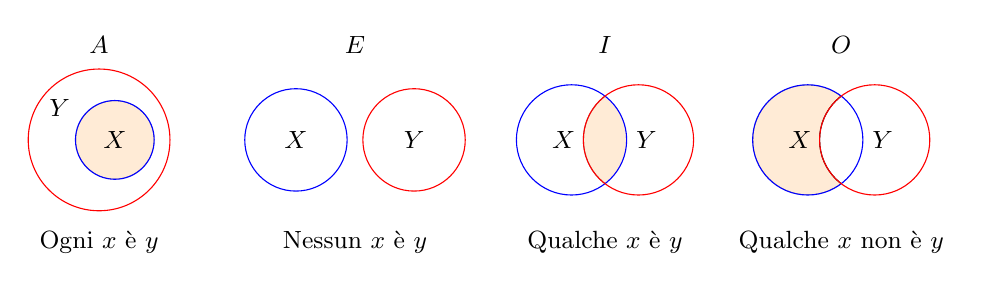
\begin{tikzpicture}[scale=1,font=\small]
\usetikzlibrary{calc}


\begin{scope}
\coordinate (oy) at (0,0);
\coordinate (ox) at (.2,0);
\draw[red] (oy) circle (0.9);

\begin{scope}
\clip (ox) circle (0.5);
\draw[fill=orange!40,opacity=.4] (ox) circle (0.5);
\end{scope}

\draw[blue] (ox) circle (.5);
\node at(.2,0){$X$};
\node at(-.5,.4){$Y$};
\node at(0,1.2){$A$};
\node at(0,-1.3){Ogni $x$ è $y$};
\end{scope}

\begin{scope}[xshift=2.5cm]
\coordinate (ox) at (0,0);
\coordinate (oy) at (1.5,0);
\draw[blue] (ox) circle (0.65);
\draw[red] (oy) circle (0.65);
\node at(0,0){$X$};
\node at(1.5,0){$Y$};
\node at(0.75,1.2){$E$};
\node at(0.75,-1.3){Nessun $x$ è $y$};
\end{scope}

\begin{scope}[xshift=6cm]
\coordinate (ox) at (0,0);
\coordinate (oy) at (0.85,0);

\begin{scope}
\clip (ox) circle (0.7);
\draw[fill=orange!40,opacity=.4] (oy) circle (0.7);
\end{scope}

\draw[blue] (ox) circle (0.7);
\draw[red] (oy) circle (0.7);

\node at(-0.1,0){$X$};
\node at(0.95,0){$Y$};
\node at(0.425,1.2){$I$};
\node at(0.425,-1.3){Qualche $x$ è $y$};
\end{scope}

\begin{scope}[xshift=9cm]
\coordinate (ox) at (0,0);
\coordinate (oy) at (0.85,0);

\begin{scope}
\clip (ox) circle (0.7);
\draw[fill=orange!40,opacity=.4] (ox) circle (0.7);
\draw[fill=white] (oy) circle (0.7);
\end{scope}

\draw[blue] (ox) circle (0.7);
\draw[red] (oy) circle (0.7);

\node at(-0.1,0){$X$};
\node at(0.95,0){$Y$};
\node at(0.425,1.2){$O$};
\node at(0.425,-1.3){Qualche $x$ non è $y$};
\end{scope}



\end{tikzpicture}
 \caption{Rappresentazione con gli insiemi di Venn dei giudizi di 
Aristotele}\label{fig:1.1}
\end{figure}
\end{inaccessibleblock}

\subsection{La dimostrazione}

Tenendo conto di quanto detto precedentemente, dimostrare che 
\(I\Rightarrow T\) significa fare un ragionamento logico che permetta 
di concludere che la tesi \(T\) è vera avendo supposto che l'ipotesi 
\(I\) sia vera.

Quando attraverso un ragionamento logico, e cioè attraverso una 
catena di implicazioni del tipo  \(I\Rightarrow A\Rightarrow 
B\Rightarrow \ldots{} \Rightarrow T\), si riesce a dedurre la verità 
di una proposizione \(T\) a partire dalla verità di una proposizione 
\(I\). Si dice che si è data una \emph{dimostrazione diretta} del 
teorema \(I\Rightarrow T\) (attraverso le regole del modus ponens e del 
sillogismo ipotetico).

Un teorema può anche essere \emph{dimostrato per assurdo}, o con 
metodo \emph{indiretto}. Questo tipo di dimostrazione consiste nel 
partire dalla negazione di \(T\) e, attraverso una catena di 
implicazioni, arrivare alla negazione di \(I\) o, in generale, ad una 
contraddizione.

Esistono altri metodi di dimostrazione, di cui eventualmente si 
parlerà più diffusamente qualora si dovesse ricorrere ad essi. Per 
ora ci limitiamo a citarne un paio: \emph{dimostrazione per 
induzione} e \emph{dimostrazione mediante esempio} o 
\emph{controesempio}.

La \emph{dimostrazione per induzione} si usa in particolare quando 
vogliamo dimostrare una proprietà generale che vale per molte 
categorie di figure ma che non si può esprimere in maniera unica per 
tutte le categorie (ad esempio una proprietà che vale per tutti i 
poligoni ma che dipende dal numero dei lati, come l'estensione dei 
criteri di congruenza dei triangoli a poligoni di più lati).

Si usa invece un \emph{esempio} quando bisogna dimostrare che una 
certa proprietà vale per almeno un oggetto del nostro studio o un 
\emph{controesempio} per dimostrare che una proprietà non vale per 
tutti gli oggetti in esame.

Per fornire alcuni esempi di dimostrazione, avremmo bisogno di 
fissare prima i concetti di base e gli assiomi da cui partire, per 
cui rinviamo la questione al prossimo paragrafo.

Ma a cosa serve studiare la dimostrazione di un teorema? Perché non 
ci limitiamo ad elencare i teoremi? Per molte applicazioni basta in 
effetti conoscere il teorema e a volte anche soltanto la formula 
risolutiva. Tuttavia studiando le dimostrazioni si impara a 
dimostrare e quindi si impara a creare nuova matematica. Un altro 
importante vantaggio è che la dimostrazione spiega perché il teorema 
è vero e permette di scoprire la struttura nascosta nelle definizioni 
e nei teoremi.

Quando si studia una dimostrazione non bisogna limitarsi a leggerla e 
a impararla a memoria, occorre leggerla attivamente, ponendo 
attenzione su cosa si fa e cercando di anticipare i passaggi. Se un 
passaggio non è chiaro bisogna prima tornare indietro per capire come 
ci si è arrivati e quindi cercare di capire il motivo per cui 
l'autore ha messo quel passaggio. In generale, una dimostrazione va 
letta più volte smettendo solo quando la si è compresa a fondo.

\vspazio\ovalbox{\risolvii \ref{ese:1.35}, \ref{ese:1.18}}

\section{Gli enti fondamentali della 
geometria}\label{sect:enti_fondamentali}

In questo paragrafo diamo un cenno del sistema assiomatico della 
geometria razionale facendo riferimento principalmente 
all'impostazione assiomatica di Hilbert.

\subsection{Concetti primitivi}

Sono concetti primitivi per la geometria il \emph{punto}, la 
\emph{retta} e il \emph{piano}. Di essi non si dà una definizione e 
costituiscono la base per definire tutti gli altri enti della 
geometria.

Oltre a questi tre enti primitivi occorre poi assumere l'esistenza di 
tre relazioni primitive tra gli enti geometrici: \emph{giacere su}, 
\emph{stare fra}, \emph{essere congruente a}. Queste relazioni 
permettono di stabilire dei legami tra gli enti geometrici, per 
esempio: <<un punto giace su una retta>>, <<un punto sta fra altri 
due punti>>, <<un segmento è congruente a un altro segmento>>, \ldots

Esiste una simbologia convenzionale, condivisa dagli studiosi, per 
indicare questi enti:
\begin{itemize}
\item per indicare un punto usiamo una lettera maiuscola: \(A\), \(B\), 
\(C\), \ldots;
\item per indicare una retta usiamo una lettera minuscola: \(a\), \(b\), 
\(c\), \ldots;
\item per indicare un piano usiamo una lettera greca: \(\alpha\), 
\(\beta\), \(\gamma\), \ldots
\end{itemize}

Ricordiamo l'alfabeto greco:
\begin{itemize}
\item lettere greche minuscole:  \(\alpha\)~(alfa),  \(\beta\)~(beta),  
\(\gamma\)~(gamma),  \(\delta\)~(delta), \(\epsilon\)~(epsilon), 
\(\zeta\)~(zeta), \(\eta\)~(eta), \(\theta\)~(theta),  \(\iota\)~(iota),  
\(\kappa\)~(kappa), \(\lambda\)~(lambda), \(\mu\)~(mi), \(\nu\)~(ni),  
\(\xi\)~(xi), \(o\)~(omicron), \(\pi\)~(pi~o~pi~greca), \(\rho\)~(rho), 
\(\sigma\)~(sigma), \(\tau\)~(tau), \(\upsilon\)~(ipsilon), \(\phi\)~(fi), 
\(\chi\)~(chi), \(\psi\)~(psi), \(\omega\)~(omega);
\item lettere greche maiuscole: \(A\), \(B\), \( \Gamma \), \( \Delta \), \( E 
\), \( Z \), \( H \), \( \Theta \), \( I \), \( K \), \( \Lambda \), \( M \), \( N \), 
\( \Xi \), \( O \), \( \Pi \), \( \Sigma \), \( T \), \( \Upsilon \), \( \Phi \), \( 
X \), \( \Psi \), \(\Omega \).
\end{itemize}

Degli enti fondamentali Euclide aveva dato le seguenti definizioni:
\begin{itemize*}
\item \emph{punto} è ciò che non ha parti;
\item \emph{linea} è lunghezza senza larghezza;
\item \emph{superficie piana} è quella che giace ugualmente rispetto 
alle rette su di essa.
\end{itemize*}
Le definizioni in questo caso sono utili per farci un'idea intuitiva 
degli enti stessi. Tuttavia, come è già stato detto in precedenza, e 
da quanto si intuisce osservando le definizioni euclidee, per 
definire il punto si utilizza la nozione di parte: ``punto è ciò che 
non ha parti''. Occorrerebbe quindi definire che cosa è una 
``parte''. Ma per definire un parte avremmo bisogno di altre nozioni 
di partenza, in un procedimento senza fine. Per questo motivo 
nell'impostazione assiomatica moderna si preferisce non dare la 
definizione dei tre enti primitivi e ``definirli implicitamente'' 
attraverso le proprietà di cui godono. Ciò significa che si 
preferisce dare maggiore importanza a come essi si comportano e cosa 
possiamo fare con essi, piuttosto che descrivere cosa sono.
Dal punto di vista della rappresentazione grafica si usano le 
convenzioni come nella figura~\ref{fig:1.2}:
%\begin{center}
% % Copyright (c) 2015 Daniele Masini - d.masini.it@gmail.com

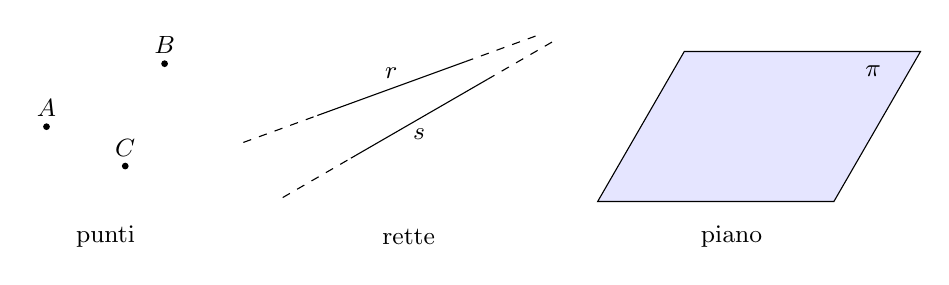
\begin{tikzpicture}[scale=1,font=\small]
\usetikzlibrary{calc}


\begin{scope}
\draw[fill] (0,0.2) circle (1pt) node[above] {$A$};
\draw[fill] (1.5,1) circle (1pt) node[above] {$B$};
\draw[fill] (1,-0.3) circle (1pt) node[above] {$C$};
\node at(.75,-1.2){punti};
\end{scope}

\begin{scope}[xshift=2.5cm]
\coordinate (d) at (0,0);
\path (d) -- +(20:1) coordinate (e);
\path (d) -- +(20:3) coordinate (f);
\path (d) -- +(20:4) coordinate (g);
\draw[dashed] (d) -- (e);
\draw[dashed] (f) -- (g);
\draw (e) -- node[above] {$r$} (f);

\coordinate (d) at (0.5,-.7);
\path (d) -- +(30:1) coordinate (e);
\path (d) -- +(30:3) coordinate (f);
\path (d) -- +(30:4) coordinate (g);

\draw[dashed] (d) -- (e);
\draw[dashed] (f) -- (g);
\draw (e) -- node[below] {$s$} (f);

\node at(2.1,-1.2){rette};
\end{scope}


\begin{scope}[xshift=4cm]
\coordinate (h) at (3,-0.75);
\path (h) -- +(60:2.2) coordinate (i);
\path (i) -- +(0:3) coordinate (l);
\path (h) -- +(0:3) coordinate (m);
\draw[fill=blue!10] (h)--(i)--(l)--(m)--cycle;
\node at(4.7,-1.2){piano};
\node at(6.5,.9){$\pi$};

\end{scope}


\end{tikzpicture}

%\end{center}

\begin{inaccessibleblock}[Figura: TODO]
 \begin{figure}[htb]
 \centering% Copyright (c) 2015 Daniele Masini - d.masini.it@gmail.com

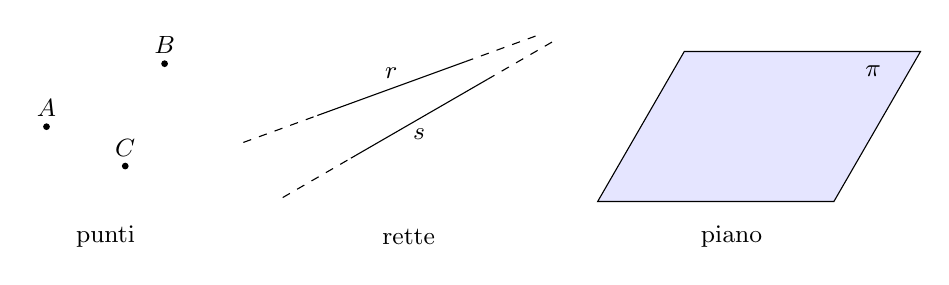
\begin{tikzpicture}[scale=1,font=\small]
\usetikzlibrary{calc}


\begin{scope}
\draw[fill] (0,0.2) circle (1pt) node[above] {$A$};
\draw[fill] (1.5,1) circle (1pt) node[above] {$B$};
\draw[fill] (1,-0.3) circle (1pt) node[above] {$C$};
\node at(.75,-1.2){punti};
\end{scope}

\begin{scope}[xshift=2.5cm]
\coordinate (d) at (0,0);
\path (d) -- +(20:1) coordinate (e);
\path (d) -- +(20:3) coordinate (f);
\path (d) -- +(20:4) coordinate (g);
\draw[dashed] (d) -- (e);
\draw[dashed] (f) -- (g);
\draw (e) -- node[above] {$r$} (f);

\coordinate (d) at (0.5,-.7);
\path (d) -- +(30:1) coordinate (e);
\path (d) -- +(30:3) coordinate (f);
\path (d) -- +(30:4) coordinate (g);

\draw[dashed] (d) -- (e);
\draw[dashed] (f) -- (g);
\draw (e) -- node[below] {$s$} (f);

\node at(2.1,-1.2){rette};
\end{scope}


\begin{scope}[xshift=4cm]
\coordinate (h) at (3,-0.75);
\path (h) -- +(60:2.2) coordinate (i);
\path (i) -- +(0:3) coordinate (l);
\path (h) -- +(0:3) coordinate (m);
\draw[fill=blue!10] (h)--(i)--(l)--(m)--cycle;
\node at(4.7,-1.2){piano};
\node at(6.5,.9){$\pi$};

\end{scope}


\end{tikzpicture}

 \caption{Rappresentazione grafica degli enti fondamentali della 
geometria}\label{fig:1.2}
\end{figure}
\end{inaccessibleblock}

\vspazio\ovalbox{\risolvi \ref{ese:1.32}}

\subsection{Postulati e assiomi}

Un \emph{postulato}, o \emph{assioma}, è una proposizione, spesso 
intuitiva, evidente ma non dimostrata, ammessa come vera in quanto 
necessaria per costruire poi le dimostrazioni dei teoremi.

Euclide nei suoi \emph{Elementi} aveva individuato un gruppo di 
cinque assiomi, che riguardano le nozioni comuni e quindi non fanno 
riferimento alla geometria, e un gruppo di cinque postulati che 
riguardano proprietà geometriche.

\paragraph{Assiomi di Euclide}
\begin{enumerate}[label=\Roman{*}.]
\item Cose che sono uguali a una stessa cosa sono uguali anche tra 
loro.
\item Se cose uguali sono addizionate a cose uguali, le totalità sono 
uguali.
\item Se da cose uguali sono sottratte cose uguali, i resti sono 
uguali.
\item Cose che coincidono fra loro sono uguali.
\item Il tutto è maggiore della parte.
\end{enumerate}

\paragraph{Postulati di Euclide}
\begin{enumerate}[label=\Roman{*}.]
\item Si possa condurre una linea retta da un qualsiasi punto ad ogni 
altro punto.
\item Un segmento si possa prolungare indefinitamente in linea retta.
\item Si possa descrivere un cerchio con qualsiasi centro e qualsiasi 
raggio.
\item Tutti gli angoli retti siano uguali tra loro.
\item Se una retta che taglia due rette forma dallo stesso lato 
angoli interni la cui somma è minore di due angoli retti, prolungando 
illimitatamente le due rette, esse si incontreranno dalla parte dove 
i due angoli sono minori di due retti.

\begin{minipage}{.49\textwidth}
\centering% Copyright (c) 2015 Daniele Masini - d.masini.it@gmail.com

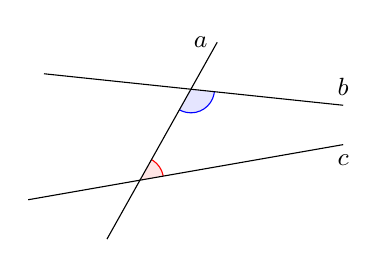
\begin{tikzpicture}[scale=1,font=\small]
\usetikzlibrary{calc}


\begin{scope}
\coordinate (c1) at (0,0);
\coordinate (c2) at (4,0.7);
\coordinate (a1) at (1,-0.5);
\coordinate (a2) at (2.4,2);
\coordinate (b1) at (0.2,1.6);
\coordinate (b2) at (4,1.2);
\coordinate (ab) at (intersection of a1--a2 and b1--b2);
\coordinate (ac) at (intersection of a1--a2 and c1--c2);

\begin{scope}
\clip (b2) -- (ab) -- (ac) -- (c2) -- cycle;
\draw[blue, fill=blue!10] (ab) circle (0.3);
\draw[red, fill=red!10] (ac) circle (0.3);
\end{scope}

\draw (a1) -- (a2) node [left] {$a$};
\draw (b1) -- (b2) node [above] {$b$};
\draw (c1) -- (c2) node [below] {$c$};

\end{scope}


\end{tikzpicture}

\end{minipage}\hfil
\begin{minipage}{.45\textwidth}
Nella figura a lato, la retta \(a\) taglia le rette \(b\) e \(c\), formando 
sul lato destro due angoli la cui somma è minore di due angoli retti. 
Prolungando opportunamente le rette \(b\) e \(c\), risulta che esse si 
incontrano sul lato destro della figura.
\end{minipage}
\end{enumerate}

Nell'impostazione assiomatica moderna di Hilbert, gli assiomi hanno 
la funzione di definire implicitamente gli enti primitivi, cioè di 
fissare le proprietà alle quali questi enti devono soddisfare. 
Hilbert aggiunge inoltre altri assiomi che Euclide stesso non aveva 
esplicitato chiaramente.

\subsubsection*{Assiomi di Hilbert}\label{sect:ass_Hilbert}

L'esposizione che segue è una semplificazione degli assiomi del 
grande matematico tedesco.\footnote{chi volesse studiare direttamente 
il testo originale può consultare 
\url{http://www.gutenberg.org/files/17384/17384-pdf.pdf} [ultima 
consultazione 20.03.2014].}

Hilbert assume come enti primitivi della geometria piana il 
\emph{punto} e la \emph{retta}, come relazioni primitive 
l'appartenenza di un punto ad una retta, il giacere di un punto tra 
altri due punti, e la congruenza di segmenti.

\paragraph{Assiomi di appartenenza} ``giacere su''
\begin{enumerate}[label=\Roman{*}.]
\item Dati due punti distinti, esiste una e una sola retta che 
contiene entrambi i punti.
\item Ogni retta contiene almeno due punti. Esistono almeno tre punti 
che non giacciono sulla stessa retta (figura~\ref{fig:1.3}).
\item Dati tre punti non allineati, esiste uno e un solo piano che 
contiene tutti e tre i punti. Ogni piano contiene almeno un punto 
(figura~\ref{fig:1.4}).
\item Se due punti di una retta giacciono su un piano, allora anche 
tutti gli altri punti della retta giacciono su questo piano 
(figura~\ref{fig:1.5}).
\item Se un punto giace su due piani distinti, allora esiste almeno 
un altro punto giacente su entrambi questi piani.
\item Esistono almeno quattro punti che non giacciono sullo stesso 
piano.
\end{enumerate}


\begin{inaccessibleblock}[Figura: TODO]
 \begin{figure}[bth]
 \begin{minipage}[b]{.32\textwidth}
 \centering
 % Copyright (c) 2015 Daniele Masini - d.masini.it@gmail.com

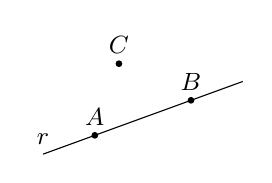
\begin{tikzpicture}[scale=1,font=\small]
\usetikzlibrary{calc}

%Assioma 2

\begin{scope}
\coordinate (o) at (0,0);
\path (o) -- +(20:0.7) coordinate (a);
\path (o) -- +(20:2) coordinate (b);
\path (o) -- +(20:2.7) coordinate (m);
\path (o) -- +(50:1.5) coordinate (c);
\path (o) -- +(30:0) coordinate (r);

\draw (o) node [above] {$r$} -- (m);
\draw[fill] (a) circle (1pt) node[above] {$A$};
\draw[fill] (b) circle (1pt) node[above] {$B$};
\draw[fill] (c) circle (1pt) node[above] {$C$};

\end{scope}

\end{tikzpicture}

 \caption{Assioma II}\label{fig:1.3}
 \end{minipage}
 \begin{minipage}[b]{.32\textwidth}
 \centering
 % Copyright (c) 2015 Daniele Masini - d.masini.it@gmail.com

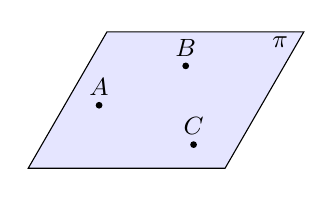
\begin{tikzpicture}[scale=1,font=\small]
\usetikzlibrary{calc}

%Assioma 3

\begin{scope}
\coordinate (d) at (0,0);
\path (d) -- +(60:2) coordinate (g);
\path (g) -- +(0:2.5) coordinate (f);
\path (d) -- +(0:2.5) coordinate (e);

\draw[fill=blue!10] (d) -- (g) -- (f) -- (e) -- cycle;
\node at (3.2,1.6){$\pi$};

\coordinate (a) at (.9,.8);
\coordinate (b) at (2,1.3);
\coordinate (c) at (2.1,.3);

\draw[fill] (a) circle (1pt) node[above] {$A$};
\draw[fill] (b) circle (1pt) node[above] {$B$};
\draw[fill] (c) circle (1pt) node[above] {$C$};

\end{scope}


\end{tikzpicture}

 \caption{Assioma III}\label{fig:1.4}
 \end{minipage}
 \begin{minipage}[b]{.32\textwidth}
 \centering
 % Copyright (c) 2015 Daniele Masini - d.masini.it@gmail.com

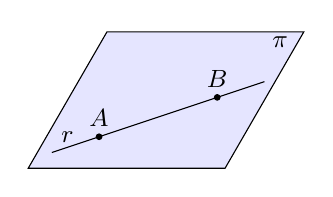
\begin{tikzpicture}[scale=1,font=\small]
\usetikzlibrary{calc}

%Assioma 4

\begin{scope}
\coordinate (d) at (0,0);
\path (d) -- +(60:2) coordinate (g);
\path (g) -- +(0:2.5) coordinate (f);
\path (d) -- +(0:2.5) coordinate (e);

\draw[fill=blue!10] (d) -- (g) -- (f) -- (e) -- cycle;
\node at (3.2,1.6){$\pi$};

\coordinate (a) at (.9,.4);
\coordinate (b) at (2.4,.9);
\draw ($(a)!-.4!(b)$) coordinate (x) node [shift={(.2,.2)}] {$r$} -- ($(a)!1.4!(b)$);

\draw[fill] (a) circle (1pt) node[above] {$A$};
\draw[fill] (b) circle (1pt) node[above] {$B$};


\end{scope}


\end{tikzpicture}

 \caption{Assioma IV}\label{fig:1.5}
 \end{minipage}
\end{figure}
\end{inaccessibleblock}

\paragraph{Assiomi di ordinamento} ``stare fra''
\begin{enumerate}[label=\Roman{*}.]
\setcounter{enumi}{6}
\item Se un punto \(B\) giace fra i punti \(A\) e \(C\), allora i punti 
\(A\), \(B\) e \(C\) sono tre punti distinti sulla stessa retta, e \(B\) 
giace fra \(C\) ed \(A\) (figura~\ref{fig:1.6}).
\item Dati due punti \(A\) e \(C\), esiste almeno un punto \(B\), sulla 
retta \(AC\), giacente fra di essi.
\item Dati tre punti qualsiasi di una retta, uno e uno solo di essi 
giace fra gli altri due.
\end{enumerate}


\begin{inaccessibleblock}[Figura: TODO]
 \begin{figure}[htb]
 \centering
 % Copyright (c) 2015 Daniele Masini - d.masini.it@gmail.com

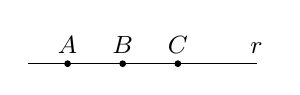
\begin{tikzpicture}[scale=1,font=\small]
\usetikzlibrary{calc}

%Assioma 7

\begin{scope}
\coordinate (o) at (0,0);
\path (o) -- +(0:.5) coordinate (a);
\path (o) -- +(0:1.2) coordinate (b);
\path (o) -- +(0:1.9) coordinate (c);
\path (o) -- +(0:2.9) coordinate (m);

\draw (o) -- (m) node [above] {$r$};

\draw[fill] (a) circle (1pt) node [above] {$A$};
\draw[fill] (b) circle (1pt) node [above] {$B$};
\draw[fill] (c) circle (1pt) node [above] {$C$};

\end{scope}

\end{tikzpicture}

 \caption{Assioma VII}\label{fig:1.6}
\end{figure}
\end{inaccessibleblock}

Gli ultimi assiomi ci permettono di dedurre il seguente teorema.
\begin{teorema}
Tra due punti di una retta esiste sempre una quantità illimitata di 
altri punti.
\end{teorema}
\begin{proof}
Data una retta \(r\) e due suoi punti \(A\) e \(B\), per l'assioma~VIII 
sappiamo che esiste un terzo punto \(C\) sulla retta \(r\) che giace tra 
\(A\) e \(B\). Ma allora esiste un punto \(D\) su \(r\) che giace tra \(A\) e 
\(C\) e un punto \(E\) che giace tra \(C\) e \(B\). Per lo stesso assioma 
esisterà un punto tra \(A\) e \(D\), uno tra \(D\) e \(C\), uno tra \(C\) e \(B\) 
e così via.
\end{proof}
\begin{center}
% Copyright (c) 2015 Daniele Masini - d.masini.it@gmail.com

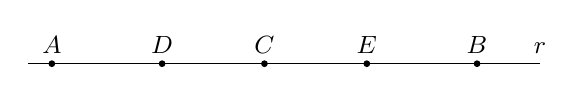
\begin{tikzpicture}[scale=1,font=\small]
\usetikzlibrary{calc}

\begin{scope}
\coordinate (l) at (0,0);
\path (l) -- +(0:.3) coordinate (a);
\path (l) -- +(0:5.7) coordinate (b);
\path (l) -- +(0:3) coordinate (c);
\path (l) -- +(0:1.7) coordinate (d);
\path (l) -- +(0:4.3) coordinate (e);
\path (l) -- +(0:6.5) coordinate (m);

\draw (l) -- (m) node [above] {$r$};

\draw[fill] (a) circle (1pt) node [above] {$A$};
\draw[fill] (b) circle (1pt) node [above] {$B$};
\draw[fill] (c) circle (1pt) node [above] {$C$};
\draw[fill] (d) circle (1pt) node [above] {$D$};
\draw[fill] (e) circle (1pt) node [above] {$E$};

\end{scope}

\end{tikzpicture}

\end{center}
\begin{definizione}
Si chiama \emph{segmento} \(AB\) l'insieme dei punti \(A\) e \(B\) e di 
tutti quelli che stanno sulla retta tra \(A\) e \(B\).
\end{definizione}
Gli assiomi di ordinamento ci permettono di dare anche la seguente

\begin{definizione}
Presi quattro punti \(A\), \(B\), \(C\), \(O\) su una retta, in modo che \(B\) 
stia tra \(A\) e \(O\) e \(O\) stia tra \(A\) e \(C\) possiamo dire che \(A\) e 
\(B\) \emph{stanno dalla medesima parte} rispetto a \(O\), mentre \(A\) e 
\(C\) non stanno dalla medesima parte rispetto a \(O\).
\end{definizione}
\begin{center}
% Copyright (c) 2015 Daniele Masini - d.masini.it@gmail.com

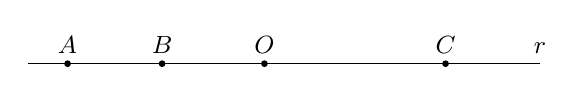
\begin{tikzpicture}[scale=1,font=\small]
\usetikzlibrary{calc}

\begin{scope}
\coordinate (l) at (0,0);
\path (l) -- +(0:.5) coordinate (a);
\path (l) -- +(0:1.7) coordinate (b);
\path (l) -- +(0:5.3) coordinate (c);
\path (l) -- +(0:3) coordinate (o);
\path (l) -- +(0:4.3) coordinate (e);
\path (l) -- +(0:6.5) coordinate (m);

\draw (l) -- (m) node [above] {$r$};

\draw[fill] (a) circle (1pt) node [above] {$A$};
\draw[fill] (b) circle (1pt) node [above] {$B$};
\draw[fill] (c) circle (1pt) node [above] {$C$};
\draw[fill] (o) circle (1pt) node [above] {$O$};

\end{scope}

\end{tikzpicture}

\end{center}

\osservazione Trascuriamo in questa trattazione elementare 
l'\emph{assioma di Pasch}\footnote{chiamato così in onore del 
matematico tedesco Moritz Pasch (1843 - 1930) che ne mise in evidenza 
l'indeducibilità dagli altri assiomi di Euclide, è uno degli assiomi 
che Hilbert aggiunse ai postulati di Euclide per renderli completi. 
Il suo enunciato è il seguente: <<Dati un triangolo nel piano, una 
retta che ne attraversi un lato in un punto che non sia un estremo, 
deve necessariamente intersecare un altro dei due lati o il vertice 
in comune tra essi.>>} (X) e l'\emph{assioma delle 
parallele}\footnote{si tratta del V postulato di Euclide, anche se 
nella tradizione didattica moderna esso viene in genere sostituito 
dall'assioma di Playfair (più restrittivo): <<Data una qualsiasi 
retta \(r\) ed un punto \(P\) non appartenente ad essa, è possibile 
tracciare per \(P\) una ed una sola retta parallela alla retta \(r\) 
data.>>} (XI).

\paragraph{Assiomi di congruenza} ``essere congruente a''
\begin{enumerate}[label=\Roman{*}.]
\setcounter{enumi}{11}
\item \emph{Assioma del trasporto di un segmento}. Se \(A\), \(B\) sono 
due punti di una retta \(r\) e \(A'\) è un punto sulla stessa retta (o 
fissato su un'altra retta \(r'\)), si può sempre trovare un punto \(B'\) 
sulla retta \(r\) (o su \(r'\)), da una data parte rispetto ad \(A'\), tale 
che il segmento \(AB\) sia congruente al segmento \(A'B'\) 
(figura~\ref{fig:1.7}).
\item La relazione di congruenza tra segmenti è transitiva, cioè se 
\(A'B'\) è congruente ad \(AB\) e \(A''B''\) è congruente ad \(AB\) allora 
\(A'B'\) è congruente ad \(A''B''\).
\item Siano \(AB\) e \(BC\) segmenti su una retta \(r\) privi di punti 
comuni a parte \(B\), e siano \(A'B'\) e \(B'C'\) segmenti su una retta 
\(r'\) privi di punti comuni a parte \(B'\). Se \(AB\cong A'B'\) e \(BC\cong 
B'C'\), allora  \(AC\cong A'C'\) (figura~\ref{fig:1.8}).
\end{enumerate}


\begin{inaccessibleblock}[Figura: TODO]
 \begin{figure}[htb]
 \begin{minipage}[b]{.5\textwidth}
 \centering
 % Copyright (c) 2015 Daniele Masini - d.masini.it@gmail.com

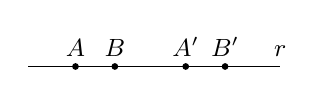
\begin{tikzpicture}[scale=1,font=\small]
\usetikzlibrary{calc}

%Assioma 12

\begin{scope}
\coordinate (l) at (0,0);
\path (l) -- +(0:.6) coordinate (a);
\path (l) -- +(0:1.1) coordinate (b);
\path (l) -- +(0:2) coordinate (a1);
\path (l) -- +(0:2.5) coordinate (b1);
\path (l) -- +(0:3.2) coordinate (m);

\draw (l) -- (m) node [above] {$r$};

\draw[fill] (a) circle (1pt) node [above] {$A$};
\draw[fill] (b) circle (1pt) node [above] {$B$};
\draw[fill] (a1) circle (1pt) node [above] {$A'$};
\draw[fill] (b1) circle (1pt) node [above] {$B'$};

\end{scope}

\end{tikzpicture}
 \caption{Assioma XII}\label{fig:1.7}
 \end{minipage}
 \begin{minipage}[b]{.5\textwidth}
 \centering
 % Copyright (c) 2015 Daniele Masini - d.masini.it@gmail.com

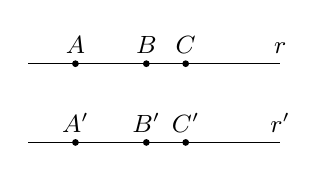
\begin{tikzpicture}[scale=1,font=\small]
\usetikzlibrary{calc}

%Assioma 14

\begin{scope}
\coordinate (l) at (0,0);
\path (l) -- +(0:.6) coordinate (a);
\path (l) -- +(0:1.5) coordinate (b);
\path (l) -- +(0:2) coordinate (c);
\path (l) -- +(0:3.2) coordinate (m);

\draw (l) -- (m) node [above] {$r$};

\draw[fill] (a) circle (1pt) node [above] {$A$};
\draw[fill] (b) circle (1pt) node [above] {$B$};
\draw[fill] (c) circle (1pt) node [above] {$C$};
\end{scope}

\begin{scope}[yshift=-1cm]
\coordinate (l) at (0,0);
\path (l) -- +(0:.6) coordinate (a);
\path (l) -- +(0:1.5) coordinate (b);
\path (l) -- +(0:2) coordinate (c);
\path (l) -- +(0:3.2) coordinate (m);

\draw (l) -- (m) node [above] {$r'$};

\draw[fill] (a) circle (1pt) node [above] {$A'$};
\draw[fill] (b) circle (1pt) node [above] {$B'$};
\draw[fill] (c) circle (1pt) node [above] {$C'$};
\end{scope}

\end{tikzpicture}

 \caption{Assioma XIV}\label{fig:1.8}
 \end{minipage}
\end{figure}
\end{inaccessibleblock}

Prima di proseguire con gli altri assiomi premettiamo le seguenti 
definizioni.
\begin{definizione}
Chiamiamo \emph{semiretta} la parte di retta costituita da un punto 
di essa, detto origine della semiretta, e da tutti i punti che stanno 
dalla stessa parte rispetto all'origine.
\end{definizione}

\begin{center}
 % Copyright (c) 2015 Daniele Masini - d.masini.it@gmail.com

\begin{tikzpicture}[scale=1,font=\small]
\usetikzlibrary{calc}

%Semiretta

\begin{scope}
\coordinate (o) at (0,0);
\path (o) -- +(0:5) coordinate (c);
\path (o) -- +(0:6) coordinate (m);

\draw (o) --  node [above] {$s$} (c);
\draw[dashed] (c) -- (m);

\draw[fill] (o) circle (1pt) node [above] {$O$};
\end{scope}

\end{tikzpicture}

\end{center}

\begin{definizione}
Si dice \emph{angolo} ciascuna delle due parti in cui un piano è 
diviso da due semirette aventi l'origine in comune; le semirette si 
dicono \emph{lati} dell'angolo; l'origine comune alle due semirette 
si dice \emph{vertice} dell'angolo (figura~\ref{fig:1.9}).
\end{definizione}
\begin{figure*}[bth]
\centering  % Copyright (c) 2015 Daniele Masini - d.masini.it@gmail.com

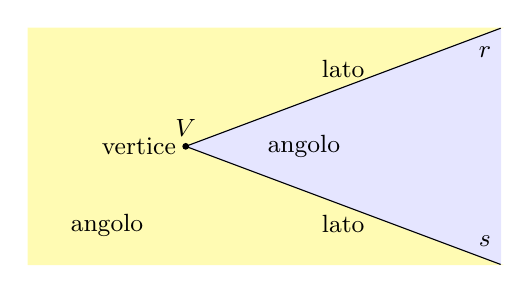
\begin{tikzpicture}[scale=1,font=\small]
\usetikzlibrary{calc}

% Angolo

\begin{scope}
\coordinate (h) at (0,0);
\coordinate (i) at (0,3);
\path (h) -- +(0:6) coordinate (m);
\path (i) -- +(0:6) coordinate (l);
\coordinate (v) at (2,1.5);
\coordinate (m1) at ($(v)!0.5!(l)$);
\coordinate (m2) at ($(v)!0.5!(m)$);

\draw[yellow!30, fill=yellow!30] (l) -- (v) -- (m) -- (h) -- (i) -- cycle;
\draw[blue!10, fill=blue!10] (l) -- (v) -- (m) -- cycle;

\draw (v) -- (l);
\draw (v) -- (m);

\draw[fill] (v) circle (1pt) node [above] {$V$};

\node at (1,.5) {angolo};
\node[left] at (v) {vertice};
\node at (3.5,1.5) {angolo};
\node[above] at (m1) {lato};
\node[below] at (m2) {lato};
\node[shift={(-.2,-.3)}] at (l) {$r$};
\node[shift={(-.2,.3)}] at (m) {$s$};

\end{scope}

\end{tikzpicture}

\caption{Le semirette \(r\) e \(s\), aventi l'origine \(V\) comune, 
individuano due regioni del piano ognuna delle quali è detta 
\emph{angolo}.}\label{fig:1.9}
\end{figure*}

L'angolo individuato da tre punti \(A\), \(B\), \(C\) è l'angolo formato 
dalla semiretta con origine \(B\) e passante per \(A\) e dalla semiretta 
con origine \(B\) e passante per \(C\). Questo angolo si indica con il 
simbolo \(A\widehat{B}C\). Nei disegni si usa indicare l'angolo con un 
archetto che indica la parte di piano considerata.

\begin{enumerate}[label=\Roman{*}.]
\setcounter{enumi}{14}
\item Dati un angolo \(A\widehat{B}C\) ed una semiretta \(B'C'\), 
esistono e sono uniche due semirette \(B'D\) e \(B'E\), tali che sia 
l'angolo \(D\widehat{B'}C'\) che \(E\widehat{B'}C'\) sono congruenti 
all'angolo \(A\widehat{B}C\) (figura~\ref{fig:1.10});

\begin{inaccessibleblock}[Figura: TODO]
 \begin{figure}[bth]
 \centering % Copyright (c) 2015 Daniele Masini - d.masini.it@gmail.com

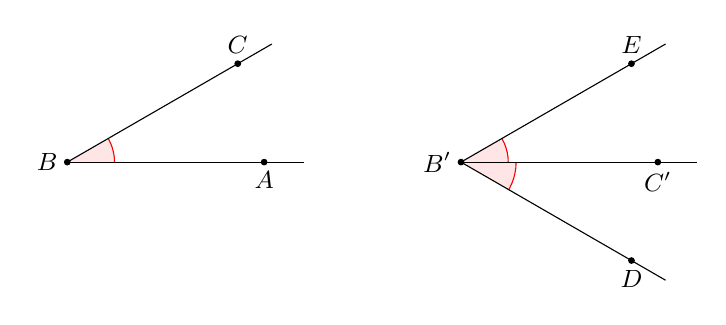
\begin{tikzpicture}[scale=1,font=\small]
\usetikzlibrary{calc}

% Assioma 15

\begin{scope}
\coordinate (b) at (0,0);
\path (b) -- +(0:2.5) coordinate (a);
\path (b) -- +(0:3) coordinate (i);
\path (b) -- +(30:2.5) coordinate (c);
\path (b) -- +(30:3) coordinate (h);

\begin{scope}
\clip (a) -- (b) -- (c) -- cycle;
\draw[red, fill=red!10] (b) circle (0.6);
\end{scope}

\draw (b) -- (h);
\draw (b) -- (i);

\draw[fill] (b) circle (1pt) node[left] {$B$};
\draw[fill] (a) circle (1pt) node[below] {$A$};
\draw[fill] (c) circle (1pt) node[above] {$C$};
\end{scope}

\begin{scope}[xshift=5cm]
\coordinate (b) at (0,0);
\path (b) -- +(0:2.5) coordinate (a);
\path (b) -- +(0:3) coordinate (i);
\path (b) -- +(30:2.5) coordinate (c);
\path (b) -- +(30:3) coordinate (h);
\path (b) -- +(-30:2.5) coordinate (d);
\path (b) -- +(-30:3) coordinate (j);

\begin{scope}
\clip (a) -- (b) -- (c) -- cycle;
\draw[red, fill=red!10] (b) circle (0.6);
\end{scope}
\begin{scope}
\clip (a) -- (b) -- (d) -- cycle;
\draw[red, fill=red!10] (b) circle (0.7);
\end{scope}

\draw (b) -- (h);
\draw (b) -- (i);
\draw (b) -- (j);

\draw[fill] (b) circle (1pt) node[left] {$B'$};
\draw[fill] (a) circle (1pt) node[below] {$C'$};
\draw[fill] (c) circle (1pt) node[above] {$E$};
\draw[fill] (d) circle (1pt) node[below] {$D$};
\end{scope}

\end{tikzpicture}

 \caption{Assioma XV}\label{fig:1.10}
\end{figure}
\end{inaccessibleblock}
\item La relazione di congruenza tra angoli è transitiva, cioè se  
\(A'\widehat{B'}C'\) e  \(A''\widehat{B''}C''\) sono congruenti ad 
\(A\widehat{B}C\), allora  \(A'\widehat{B'}C' \equiv 
A''\widehat{B''}C''\).
\end{enumerate}

\paragraph{Assioma di continuità}

\begin{enumerate}[label=\Roman{*}.]
\setcounter{enumi}{16}
\item \emph{Assioma di Archimede}. Sulla retta che unisce due punti 
qualsiasi \(A\) e \(B\) si prende un punto \(A_1\), quindi si prendono i 
punti \(A_2\), \(A_3\), \(A_4\), \ldots in modo che \(A_1\) sia tra \(A\) e 
\(A_2\), \(A_2\) tra \(A_1\) e \(A_3\), \(A_3\) tra \(A_2\) e \(A_4\), ecc. e che  
\(AA_1\equiv A_1A_2\equiv A_2A_3\equiv A_3A_4\equiv\ldots\) allora tra 
tutti questi punti esiste sempre un punto \(A_n\) tale che \(B\) sta tra 
\(A\) e \(A_n\) (figura~\ref{fig:1.11}).

\begin{inaccessibleblock}[Figura: TODO]
 \begin{figure}[bth]
 \centering % Copyright (c) 2015 Daniele Masini - d.masini.it@gmail.com

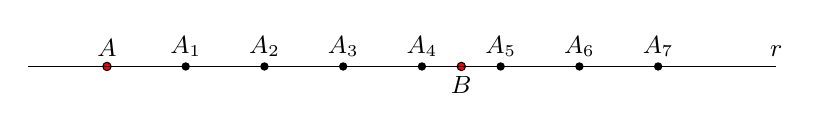
\begin{tikzpicture}[scale=1,font=\small]
\usetikzlibrary{calc}

% Assioma 17

\begin{scope}
\coordinate (l) at (-1,0);
\coordinate (m) at (8.5,0);
\foreach \x in {1, 2, ..., 7}
{
\draw[fill] ({\x},0) circle (1.3pt) node[above] {$A_{\x}$};
}

\draw[fill=red] (0,0) circle (1.5pt) node[above] {$A$};
\draw[fill=red] (4.5,0) circle (1.5pt) node[below] {$B$};
\draw (l) -- (m) node[above] {$r$};

\end{scope}

\end{tikzpicture}

 \caption{Assioma di Archimede (XVII)}\label{fig:1.11}
\end{figure}
\end{inaccessibleblock}
\end{enumerate}

\paragraph{Assioma di completezza}

\begin{enumerate}[label=\Roman{*}.]
\setcounter{enumi}{17}
\item Ad un sistema di punti, linee rette e piani è impossibile 
aggiungere altri elementi in modo tale che il sistema, così 
generalizzato, formi una nuova geometria obbediente a tutti i cinque 
gruppi di assiomi. In altre parole, gli elementi della geometria 
formano un sistema che non è suscettibile di estensione, nel caso in 
cui si considerino validi i cinque gruppi di assiomi.
\end{enumerate}

\vspazio\ovalbox{\risolvii \ref{ese:1.33}, \ref{ese:1.34}, 
\ref{ese:1.36}, \ref{ese:1.37}, \ref{ese:1.38}, \ref{ese:1.39}, 
\ref{ese:1.40}, \ref{ese:1.41}, \ref{ese:1.42}}


\section{Prime definizioni}\label{sect:prime_definizioni}

\subsection{Semirette e segmenti}

Nel paragrafo precedente abbiamo già introdotto alcune definizioni di 
base, necessarie per enunciare tutti i postulati della geometria 
secondo l'assiomatizzazione di Hilbert. In questo paragrafo 
costruiamo le prime definizioni. Per comodità del lettore riportiamo 
anche quelle già date.

Partiamo dalla nozione generica di figura.
\begin{definizione}
Si chiama \emph{figura} un qualsiasi insieme, non vuoto, di punti.
\end{definizione}
Questa definizione fa riferimento soltanto all'ente primitivo 
geometrico di punto.

Lo spazio non è considerato un ente primitivo, in quanto può essere 
ottenuto dalla seguente definizione.
\begin{definizione}
Si chiama \emph{spazio} l'insieme di tutti i punti.
\end{definizione}
Risulta pertanto che una figura è un qualsiasi sottoinsieme dello 
spazio.

In base agli assiomi di ordinamento un qualunque punto \(P\) su una 
retta divide la retta in due parti, una è costituita dai punti che 
``seguono'' \(P\), l'altra è costituita dai punti che ``precedono'' \(P\).
\begin{definizione}
Si chiama \emph{semiretta} la parte di retta costituita da un punto 
di essa, detto origine della semiretta, e da tutti i punti che stanno 
dalla stessa parte rispetto all'origine.
\end{definizione}
Solitamente una semiretta viene indicata con una lettera latina 
minuscola.

Prendendo due qualsiasi rette dello spazio esse si possono trovare in 
diverse posizioni reciproche, cioè una rispetto all'altra.
\begin{definizione}
Due rette che appartengono ad uno stesso piano si dicono 
\emph{complanari}, altrimenti si dicono \emph{sghembe}.
\end{definizione}

\begin{definizione}
Due rette complanari \(r\) ed \(s\) che non hanno nessun punto in comune 
si dicono \emph{parallele} e si scrive \(r\parallel s\).
\end{definizione}

\begin{definizione}
Due rette che hanno un solo punto in comune si dicono 
\emph{incidenti}.
\end{definizione}

\begin{definizione}
Se due rette hanno almeno due punti in comune sono \emph{coincidenti}.
\end{definizione}


\begin{inaccessibleblock}[Figura: TODO]
 \begin{figure}[hbt]
 \centering % Copyright (c) 2015 Daniele Masini - d.masini.it@gmail.com

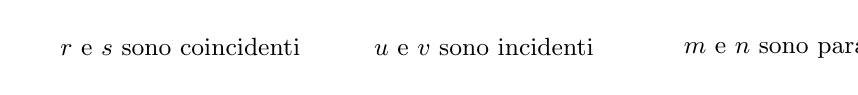
\begin{tikzpicture}[font=\small]
%rette coincidenti
\tkzDefPoint(0,0){A}
\tkzDefShiftPoint[A](20:3){B}
%\tkzDefPoint(0,-.05){C}
%\tkzDefShiftPoint[C](20:3){D}
\tkzLabelPoint[font=\small,above](B){$r$}
\tkzLabelPoint[font=\small,below](B){$s$}
%\tkzDrawSegments(A,B C,D)
\tkzDrawSegments(A,B)
\node at(1.5,-1){$r$ e $s$ sono coincidenti};

%rette incidenti
\tkzDefPoint(3.5,0){A}
\tkzDefShiftPoint[A](20:3){B}
\tkzDefPoint(4,-.3){C}
\tkzDefShiftPoint[C](40:2.5){D}
\tkzLabelPoint[font=\small,below](B){$ v $}
\tkzLabelPoint[font=\small,above](D){$ u $}
\tkzDrawSegments(A,B C,D)
\node at(5,-1){$ u $ e $ v $ sono incidenti};

%rette parallele
\tkzDefPoint(7,0){A}
\tkzDefShiftPoint[A](30:3){B}
\tkzDefPoint(7.5,-.3){C}
\tkzDefShiftPoint[C](30:3){D}
\tkzLabelPoint[font=\small,above](B){$ m $}
\tkzLabelPoint[font=\small,below](D){$ n $}
\tkzDrawSegments(A,B C,D)
\node at(8.5,-1){$ m $ e $ n $ sono parallele};
\end{tikzpicture}

 \caption{Relazioni tra rette complanari}\label{fig:1.12}
\end{figure}
\end{inaccessibleblock}

\osservazione Due rette non parallele possono appartenere a piani 
diversi, in questo caso non avranno punti in comune, sono cioè 
sghembe. Viceversa se due rette hanno un punto in comune allora sono 
sicuramente complanari. Inoltre, se hanno più di un punto in comune 
le rette coincidono, in questo caso ci sono infiniti piani che le 
contengono. 


\begin{inaccessibleblock}[Figura: TODO]
 \begin{figure}[!htb]
	\centering% Copyright (c) 2015 Daniele Masini - d.masini.it@gmail.com

\begin{tikzpicture}[font=/small]
\tkzDefPoint(0,0){O}
%\tkzDefPoint(2,0){A}
\foreach \ang in {30,60,...,360}{%
\tkzDefPoint(\ang:1.3){M}
\tkzDrawSegment(M,O)
}
\end{tikzpicture}

	\caption{Fascio proprio di rette}\label{fig:1.16}
\end{figure}
\end{inaccessibleblock}

\begin{definizione}
L'insieme di tutte le rette di un piano che passano per uno stesso 
punto è detto \emph{fascio proprio di rette}, il punto in comune a 
tutte le rette si dice \emph{centro del fascio} 
(figura~\ref{fig:1.16}).
\end{definizione}

Prendendo su una retta due punti \(A\) e \(B\), la retta resta divisa in 
tre parti: la semiretta di origine \(A\) che non contiene \(B\), la parte 
costituita dai punti compresi tra \(A\) e \(B\) e la semiretta di origine 
\(B\) che non contiene \(A\).

\begin{definizione}
Si chiama \emph{segmento} \(AB\) l'insieme dei punti \(A\) e \(B\) e di 
tutti quelli che stanno tra \(A\) e \(B\).
I punti \(A\) e \(B\) si dicono \emph{estremi} del segmento.
\end{definizione}
Un segmento viene indicato con le due lettere maiuscole dei suoi 
estremi.

\begin{inaccessibleblock}[Figura: TODO]
 \begin{figure}[bth]
 \centering % Copyright (c) 2015 Daniele Masini - d.masini.it@gmail.com

\begin{tikzpicture}[font=\small]
%definizione di segmento
\tkzDefPoint(0,0){r}
\tkzDefShiftPoint[r](0:9){s}
\tkzDefShiftPoint[r](0:3){A}
\tkzDefShiftPoint[r](0:6){B}
\tkzDefPoint(1.5,.5){e1}
\tkzDefPoint(7.5,.5){e2}
\tkzDefPoint(4.5,0){p}
\tkzDefPoint(1.5,-.5){s1}
\tkzDefPoint(7.5,-.5){s2}
\tkzDrawSegments[style=dashed](r,A B,s)
\tkzDrawSegment[very thick](A,B)
\tkzDrawPoints[fill=red](A,B)
\tkzLabelPoints[font=\small,above](r,s)
\tkzLabelPoints[font=\small,above](A,B)
\tkzLabelPoint[font=\small,above](p){punti interni}
\tkzLabelPoint[font=\small,below](4.5,-.5){segmento $AB$}
\tkzLabelPoint[font=\small,below](s1){semiretta di origine $A$}
\tkzLabelPoint[font=\small,below](s2){semiretta di origine $B$}
\tkzLabelPoint[font=\small,above](e1){estremo}
\tkzLabelPoint[font=\small,above](e2){estremo}
\tkzDefPoint(2.9,0.1){a1}
\tkzDefPoint(6.1,0.1){b1}
\tkzDrawSegments[thick,dotted,->,-latex](e1,a1 e2,b1)
\tkzDrawSegment[thick,dotted,->,-latex]({4.5,-.5},{4.5,-0.1})
%\draw[thick,dotted,->,-latex](0.5,-0.5).. controls (2,-.2)..(1,0);
%\draw[thick,dotted,->,-latex](8.5,-0.5).. controls (7,-.2)..(8,0);
\tkzDefPoint(1.5,-0.1){rm}
\tkzDrawSegments[thick,dotted,->,-latex](s1,rm)
\tkzDefPoint(7.5,-0.1){sm}
\tkzDrawSegments[thick,dotted,->,-latex](s2,sm)
\end{tikzpicture}

 \caption{I punti \(A\) e \(B\) formano le due semirette \(r\) ed \(s\), e il 
segmento \(AB\)}\label{fig:1.13}
\end{figure}
\end{inaccessibleblock}

Due segmenti nel piano possono trovarsi in diverse posizioni 
reciproche. Alcune di esse hanno un interesse per la geometria.
\begin{definizione}
Due segmenti si dicono \emph{consecutivi} se hanno in comune soltanto 
un estremo (figura~\ref{fig:1.14}).
\end{definizione}

\begin{inaccessibleblock}[Figura: TODO]
 \begin{figure}[bth]
 \centering % Copyright (c) 2015 Daniele Masini - d.masini.it@gmail.com

\begin{tikzpicture}[font=\small]
%segmenti consecutivi
\tkzDefPoint(0,0){B}
\tkzDefShiftPoint[B](120:2){A}
\tkzDefShiftPoint[B](0:2.5){C}
\tkzDrawPoints(A,B,C)
\tkzLabelPoints[font=\small](B,C)
\tkzLabelPoint[font=\small,right](A){A}
\tkzDrawSegments(A,B B,C)
\node at(1.25,-.7){segmenti consecutivi};

%non consecutivi
\tkzDefPoint(4,0){E}
\tkzDefShiftPoint[E](120:.7){F}
\tkzDefShiftPoint[E](120:2){D}
\tkzDefShiftPoint[F](10:2.5){G}
\tkzDrawPoints(E,F,D,G)
\tkzLabelPoints[font=\small,left](E,F,D)
\tkzLabelPoint[font=\small,above](G){G}
\tkzDrawSegments(E,D F,G)
\node at(6.5,-.7){Segmenti non consecutivi};

\tkzDefPoint(7,0){H}
\tkzDefShiftPoint[H](100:2){I}
\tkzDefShiftPoint[H](60:1.5){L}
\tkzDefShiftPoint[H](10:3){M}
\tkzDrawPoints(H,I,L,M)
\tkzLabelPoints[font=\small,right](H,I)
\tkzLabelPoints[font=\small,above](L,M)
\tkzDrawSegments(H,I L,M)
\end{tikzpicture}

 \caption{I segmenti \(AB\) e \(BC\) sono consecutivi perché hanno in 
comune solo il punto~\(B\) che è un estremo di entrambi; \(DE\) e \(FG\) 
non sono consecutivi perché hanno in comune solo il punto \(F\) ma esso 
non è estremo del segmento \(DE\); \(HI\) e \(LM\) non sono consecutivi 
perché non hanno nessun punto in comune.}\label{fig:1.14}
\end{figure}
\end{inaccessibleblock}

\begin{definizione}
Due segmenti si dicono \emph{adiacenti} se sono consecutivi ed 
appartengono alla stessa retta (figura~\ref{fig:1.15}).
\end{definizione}

\begin{inaccessibleblock}[Figura: TODO]
 \begin{figure}[tbh]
 \centering % Copyright (c) 2015 Daniele Masini - d.masini.it@gmail.com

\begin{tikzpicture}[font=\small]
%segmenti adiacenti
\tkzDefPoint(0,0){A}
\tkzDefShiftPoint[A](60:1.5){B}
\tkzDefShiftPoint[A](60:2.5){C}
\tkzDrawPoints(A,B,C)
\tkzLabelPoints[font=\small,right](A,B,C)
\tkzDrawSegment(A,C)
\node at(.3,-.5){segmenti adiacenti};

%non consecutivi
\tkzDefPoint(4,0){D}
\tkzDefShiftPoint[D](60:.7){E}
\tkzDefShiftPoint[D](60:1.7){F}
\tkzDefShiftPoint[D](60:2.5){G}
\tkzDrawPoints(E,F,D,G)
\tkzLabelPoints[font=\small,right](D,E,F,G)
\tkzDrawSegments(E,D F,G)
\tkzDrawSegment[dashed](E,F)
\node at(5.5,-.5){Segmenti non adiacenti};

\tkzDefPoint(7,0){H}
\tkzDefShiftPoint[H](60:1){L}
\tkzDefShiftPoint[H](60:1.5){I}
\tkzDefShiftPoint[H](60:2.5){M}
\tkzDrawPoints(H,I,L,M)
\tkzLabelPoints[font=\small,right](H,I,L,M)
\tkzDrawSegment(H,M)
\end{tikzpicture}

 \caption{I segmenti \(AB\) e \(BC\) sono adiacenti perché hanno in 
comune solo l'estremo \(B\) e giacciono sulla stessa retta; i segmenti 
\(DE\) e \(FG\), pur giacendo sulla stessa retta, non sono adiacenti 
poiché non hanno alcun punto in comune; i segmenti \(HI\) e \(LM\) 
giacciono sulla stessa retta ma non sono adiacenti poiché hanno più 
di un punto in comune.}\label{fig:1.15}
\end{figure}
\end{inaccessibleblock}

\ovalbox{\risolvii \ref{ese:1.43}, \ref{ese:1.44}, \ref{ese:1.45}, 
\ref{ese:1.46}, \ref{ese:1.47}, \ref{ese:1.48}, \ref{ese:1.49}, 
\ref{ese:1.50}}

\subsection{Semipiani e angoli}

\begin{definizione}
Si dice \emph{semipiano} di origine la retta \(r\) la figura formata 
dalla retta \(r\) e da una delle due parti in cui essa divide il piano 
(figura~\ref{fig:1.17}).
\end{definizione}

\begin{inaccessibleblock}[Figura: TODO]
 \begin{figure}[bth]
 \centering% Copyright (c) 2015 Daniele Masini - d.masini.it@gmail.com

\begin{tikzpicture}[font=\small]
%semipiani
\tkzDefPoint(0,0){D}
\tkzDefShiftPoint[D](50:2){G}
\tkzDefShiftPoint[G](0:2.5){F}
\tkzDefShiftPoint[D](0:2.5){E}
\tkzDefShiftPoint[D](50:.7){L}
\tkzDefMidPoint(F,E) \tkzGetPoint{M}
\tkzLabelPoint[right](M){$r$}
\tkzLabelPoint[right](F){$\pi$}
\tkzDrawPolygon[thin,blue,fill=blue!10](L,G,F,M)
\tkzDrawPolygon[thin,blue,fill=yellow!30](D,L,M,E)
\tkzDrawSegment[thick](L,M)
\node at(1.6,.3){semipiano};
\node at(2.1,1.2){semipiano};
\end{tikzpicture}

  \caption{Semipiani opposti}\label{fig:1.17}
\end{figure}
\end{inaccessibleblock}
In un piano \({\pi}\), una qualsiasi retta \(r \subset \pi\) dà origine a 
due semipiani distinti, che si dicono semipiani \emph{opposti}.

\begin{definizione}
Una figura si dice \emph{convessa} se, considerati due suoi qualsiasi 
punti, il segmento che li unisce è contenuto nella figura. Si dice 
\emph{concava} se esistono almeno due punti per i quali il segmento 
che li unisce non è interamente contenuto nella figura 
(figura~\ref{fig:1.18}).
\end{definizione}

\begin{inaccessibleblock}[Figura: TODO]
 \begin{figure}[bth]
 \centering % Copyright (c) 2015 Daniele Masini - d.masini.it@gmail.com

\begin{tikzpicture}[font=\small]
%convesso
\tkzDefPoints{0/1/A,
1.4/.8/B,
3.5/2/C,
1.6/3.2/D,
.6/2/E}
\tkzDefShiftPoint[A](30:.5){A1}
\tkzDefShiftPoint[A1](40:2.1){D1}
\tkzDefShiftPoint[A1](5:.5){A2}
\tkzDefShiftPoint[A1](10:2.1){D2}
\tkzLabelPoint[below,font=\small](1.8,0.85){$F$}
%concavo
\tkzDefPoints{5/2.6/H,
5.8/3/I,
7/2/L,
8.2/2.8/M,
8.5/1.3/N,
8/.3/O,
7/.2/P,
6/.3/Q,
5/.8/R,
5.2/1.7/S}
\tkzDefShiftPoint[H](-3:.7){H1}
\tkzDefShiftPoint[M](-110:.6){M1}
\tkzDefShiftPoint[H](-60:.7){H2}
\tkzDefShiftPoint[L](-40:1){L1}
\tkzDefShiftPoint[R](-10:.5){Q1}
\tkzDefShiftPoint[Q1](10:2.5){Q2}
\tkzLabelPoint[below,font=\small](6.7,0.2){$G$}

\tkzDrawPolygon[fill=blue!10,rounded corners](A,B,C,D,E)
\tkzDrawPolygon[fill=yellow!30,rounded corners](H,I,L,M,N,O,P,Q,R,S)
\tkzDrawSegments(A1,D1 A2,D2 H1,M1 H2,L1 Q1,Q2)
\tkzDrawPoints(A1,D1,A2,D2,H1,M1,H2,L1,Q1,Q2)
\tkzLabelPoint[below,font=\small](H1){$P$}
\tkzLabelPoint[below,font=\small](M1){$Q$}

\end{tikzpicture}


 \caption{La figura \( F \) è convessa, per qualsiasi coppia di punti 
interni a \( F \) il segmento che li unisce è interamente nella figura; 
la figura \( G \) è concava perché unendo i punti \( P \) e \( Q \) si ha 
un segmento che cade in parte esternamente alla 
figura.}\label{fig:1.18}
\end{figure}
\end{inaccessibleblock}

Ricordiamo la definizione di angolo già data: si dice \emph{angolo} 
ciascuna delle due parti in cui un piano è diviso da due semirette 
aventi l'origine in comune; le semirette si dicono \emph{lati} 
dell'angolo; l'origine comune alle due semirette si dice 
\emph{vertice} dell'angolo (figura~\ref{fig:1.9}).

\begin{definizione}
Un angolo si dice \emph{piatto} se i suoi lati sono uno il 
prolungamento dell'altro.
\end{definizione}

\begin{definizione}
Un angolo si dice \emph{nullo} se è costituito solo da due semirette 
sovrapposte.
\end{definizione}

\begin{definizione}
\`E detto \emph{angolo giro} l'angolo che ha per lati due semirette 
sovrapposte e che contiene tutti i punti del piano 
(figura~\ref{fig:1.19}).
\end{definizione}

\begin{inaccessibleblock}[Figura: TODO]
 \begin{figure}[bth]
 \centering % Copyright (c) 2015 Daniele Masini - d.masini.it@gmail.com

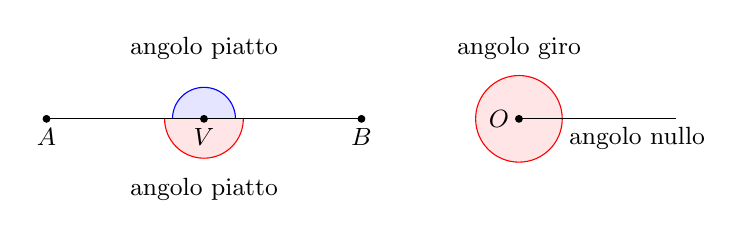
\begin{tikzpicture}[scale=1,font=\small]
\usetikzlibrary{calc}

%angolo piatto
\begin{scope}
\coordinate (a) at (-2,0);
\coordinate (b) at (2,0);
\coordinate (v) at (0,0);

\begin{scope}
\clip (a) -- (-.6,.6) -- (.6,.6) -- (b) -- cycle;
\draw[blue, fill=blue!10] (v) circle (0.4);
\end{scope}

\begin{scope}
\clip (a) -- (-.6,-.6) -- (.6,-.6) -- (b) -- cycle;
\draw[red, fill=red!10] (v) circle (0.5);
\end{scope}

\draw (a) -- (b);
\draw[fill] (a) circle (1.2pt) node [below] {$A$};
\draw[fill] (b) circle (1.2pt) node [below] {$B$};
\draw[fill] (v) circle (1.2pt) node [below] {$V$};

\node at (0,0.9) {angolo piatto};
\node at (0,-0.9) {angolo piatto};

\end{scope}


%angolo giro/nullo
\begin{scope}[xshift=4cm]
\coordinate (a) at (2,0);
\coordinate (v) at (0,0);

\draw[red, fill=red!10] (v) circle (0.55);
\draw (v) -- (a);
%\draw[fill] (a) circle (1.2pt) node [below] {$A$};
\draw[fill] (v) circle (1.2pt) node [left] {$O$};

\node at (0,0.9) {angolo giro};
\node at (1.5,-0.25) {angolo nullo};

\end{scope}

\end{tikzpicture}

 \caption{L'angolo  \(\widehat{ab}\) a sinistra è piatto (sia quello 
sopra che quello sotto), gli angoli a destra, individuati dalle 
semirette coindicenti con origine in \(O\), sono rispettivamente un 
angolo giro (quello esterno) e un angolo nullo (quello 
interno).}\label{fig:1.19}
\end{figure}
\end{inaccessibleblock}

\begin{definizione}
Un angolo, i cui lati non appartengono alla stessa retta, si dice 
\emph{concavo} se contiene i prolungamenti dei lati, se non li 
contiene si dice \emph{convesso}.
\end{definizione}

\begin{figure*}[htb]
\centering  % Copyright (c) 2015 Daniele Masini - d.masini.it@gmail.com

\begin{tikzpicture}
%angolo1
\tkzDefPoint(0,0){H}
\tkzDefPoint(0,3){I}
\tkzDefShiftPoint[H](0:6){M}
\tkzDefShiftPoint[I](0:6){L}
\tkzDefPoint(2,1.5){V}
\tkzDefMidPoint(V,L)	\tkzGetPoint{M1}
\tkzDefMidPoint(V,M)	\tkzGetPoint{M2}
\tkzDrawSegments(V,L V,M)
\tkzFillPolygon[yellow!30](L,V,M,H,I)
\tkzFillPolygon[blue!30,opacity=.25](L,V,M)
%\tkzDrawSegment[style=dashed](C,M)
\tkzDrawPoint(V)

\begin{scope}
\clip(0,0) rectangle (3,3);
\tkzDefShiftPoint[H](0:-3){M1}
\tkzDefShiftPoint[I](0:-3){L1}
\tkzDrawSegments[dotted](V,M1 V,L1)
\end{scope}

\tkzLabelPoint[above right](0.7,.3){angolo concavo}
\tkzLabelPoint[right](3,1.5){angolo convesso}

\end{tikzpicture}

\caption{L'angolo concavo è quello in giallo in quanto contiene i 
prolungamenti dei lati (punteggiati)}\label{fig:1.20}
\end{figure*}

Quando si disegna un angolo è utile, oltre a disegnare le semirette e 
l'origine, indicare con un archetto quale dei due angoli si intende 
considerare.


\begin{inaccessibleblock}[Figura: TODO]
 \begin{figure}[htb]
 \centering % Copyright (c) 2015 Daniele Masini - d.masini.it@gmail.com

\begin{tikzpicture}
%assioma 15
\tkzDefPoint(0,0){O}
\tkzDefShiftPoint[O](0:2.5){B}
\tkzDefShiftPoint[O](0:3){I}
\tkzDefShiftPoint[O](30:2.5){A}
\tkzDefShiftPoint[O](30:3){H}
\tkzDrawPoints(A,O,B)
\tkzDrawSegments(O,H O,I)
\tkzLabelPoints[font=\small, left](O)
\tkzLabelPoints[font=\small, above](A)
\tkzLabelPoints[font=\small, below](B)
\tkzMarkAngle[fill=orange,opacity=.3,size=1cm](B,O,A)
\tkzLabelPoint[font=\small,right](19:0.95){$\alpha$}
\tkzLabelPoint[font=\small,above](30:3){$a$}
\tkzLabelPoint[font=\small,below](0:3){$b$}
\end{tikzpicture}

\caption{Per indicare che l'angolo da considerare è quello convesso e 
non quello concavo si è usato un archetto in prossimità del vertice 
\(O\)}\label{fig:1.21}
\end{figure}
\end{inaccessibleblock}

Per indicare gli angoli si usano diverse convenzioni:
\begin{itemize*}
\item  \(\widehat{ab}\): se si conoscono i nomi delle semirette che ne 
costituiscono i lati;
\item  \(A\widehat{O}B\): se si conoscono i nomi del vertice e di due 
punti sui lati;
\item  \(\alpha\), \(\beta\), \(\gamma\), \ldots{} (una lettera greca): per 
indicare direttamente l'angolo.
\end{itemize*}
I primi due modi di indicare l'angolo non individuano con chiarezza 
di quale dei due angoli si tratta. Solitamente si intende l'angolo 
convesso, quando si vuole indicare l'angolo concavo bisogna dirlo 
esplicitamente.

Anche per gli angoli si danno le definizioni di angoli consecutivi e 
angoli adiacenti, in parte simili a quelle date per i segmenti.

\begin{definizione}
Due angoli si dicono \emph{consecutivi} se hanno il vertice e un lato 
comune e giacciono da parte opposta rispetto al lato comune.
\end{definizione}


\begin{inaccessibleblock}[Figura: TODO]
 \begin{figure}[htb]
 \centering % Copyright (c) 2015 Daniele Masini - d.masini.it@gmail.com

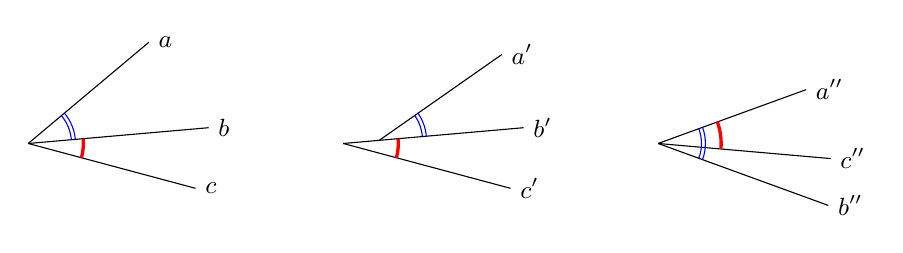
\begin{tikzpicture}
\pgfmathsetmacro{\myscale}{1};

\begin{scope}[scale={\myscale},font=\small]
\usetikzlibrary{calc}

\begin{scope}
\pgfmathsetmacro{\aalpha}{40};
\pgfmathsetmacro{\abeta}{5};
\pgfmathsetmacro{\agamma}{-15};

\coordinate (o) at (0,0);
\draw (o) -- ++({\aalpha}:2) coordinate (a) node[right] {$a$};
\draw (o) -- ++({\abeta}:2.3) coordinate (b) node[right] {$b$};
\draw (o) -- ++({\agamma}:2.2) coordinate (c) node[right] {$c$};

\draw[thin,blue] ([shift=({\abeta}:.55)]o) arc [radius=.55, start angle={\abeta}, end angle={\aalpha}];
\draw[thin,blue] ([shift=({\abeta}:.6)]o) arc [radius=.6, start angle={\abeta}, end angle={\aalpha}];
\draw[very thick, red] ([shift=({\agamma}:.7)]o) arc [radius =.7, start angle={\agamma}, end angle={\abeta}];
\end{scope}

\pgfmathsetmacro{\myxshift}{4cm};
\begin{scope}[xshift={\myxshift}]
\pgfmathsetmacro{\aalpha}{35};
\pgfmathsetmacro{\abeta}{5};
\pgfmathsetmacro{\agamma}{-15};

\coordinate (o) at (0,0);
\draw (o) -- ++({\abeta}:2.3) coordinate (b) node[right] {$b'$};
\draw (o) -- ++({\agamma}:2.2) coordinate (c) node[right] {$c'$};
\coordinate (u) at ($(o)!0.2!(b)$);
\draw (u) -- ++({\aalpha}:1.9) coordinate (a) node[right] {$a'$};

\draw[thin,blue] ([shift=({\abeta}:.55)]u) arc [radius=.55, start angle={\abeta}, end angle={\aalpha}];
\draw[thin,blue] ([shift=({\abeta}:.6)]u) arc [radius=.6, start angle={\abeta}, end angle={\aalpha}];
\draw[very thick, red] ([shift=({\agamma}:.7)]o) arc [radius =.7, start angle={\agamma}, end angle={\abeta}];
\end{scope}

\pgfmathsetmacro{\myxshift}{8cm};
\begin{scope}[xshift={\myxshift}]
\pgfmathsetmacro{\aalpha}{20};
\pgfmathsetmacro{\abeta}{-20};
\pgfmathsetmacro{\agamma}{-5};

\coordinate (o) at (0,0);
\draw (o) -- ++({\aalpha}:2) coordinate (a) node[right] {$a''$};
\draw (o) -- ++({\abeta}:2.3) coordinate (b) node[right] {$b''$};
\draw (o) -- ++({\agamma}:2.2) coordinate (c) node[right] {$c''$};

\draw[thin,blue] ([shift=({\abeta}:.55)]o) arc [radius=.55, start angle={\abeta}, end angle={\aalpha}];
\draw[thin,blue] ([shift=({\abeta}:.6)]o) arc [radius=.6, start angle={\abeta}, end angle={\aalpha}];
\draw[very thick, red] ([shift=({\agamma}:.8)]o) arc [radius =.8, start angle={\agamma}, end angle={\aalpha}];
\end{scope}

\end{scope}
\end{tikzpicture}

\caption{Nella figura gli angoli  \(\widehat{ab}\) e \(\widehat{bc}\)  
sono consecutivi perché hanno il vertice e il lato \( b \) in comune;  
\(\widehat {a'b'}\) e \(\widehat {b'c'}\)  non sono consecutivi perché 
non hanno il vertice in comune;  \(\widehat {a''b''}\) e \(\widehat 
{a''c''}\) non sono consecutivi perché non giacciono da parti opposte 
rispetto al lato in comune \(a''\)}\label{fig:1.22}
\end{figure}
\end{inaccessibleblock}

\begin{definizione}
Due angoli si dicono \emph{adiacenti} se sono consecutivi e se i lati 
non comuni giacciono sulla stessa retta.
\end{definizione}


\begin{inaccessibleblock}[Figura: TODO]
 \begin{figure}[htb]
 \centering % Copyright (c) 2015 Daniele Masini - d.masini.it@gmail.com

\begin{tikzpicture}
\pgfmathsetmacro{\myscale}{1};

\begin{scope}[scale={\myscale},font=\small]
\usetikzlibrary{calc}

\begin{scope}
\pgfmathsetmacro{\aalpha}{0};
\pgfmathsetmacro{\abeta}{40};
\pgfmathsetmacro{\agamma}{180};

\coordinate (o) at (0,0);
\draw (o) -- ++({\aalpha}:2.2) coordinate (a) node[right] {$a$};
\draw (o) -- ++({\abeta}:2) coordinate (b) node[right] {$b$};
\draw (o) -- ++({\agamma}:2) coordinate (c) node[left] {$c$};

\draw[thin,blue] ([shift=({\abeta}:.65)]o) arc [radius=.65, start angle={\abeta}, end angle={\aalpha}];
\draw[thin,blue] ([shift=({\abeta}:.7)]o) arc [radius=.7, start angle={\abeta}, end angle={\aalpha}];
\draw[very thick, red] ([shift=({\agamma}:.5)]o) arc [radius =.5, start angle={\agamma}, end angle={\abeta}];
\end{scope}


\pgfmathsetmacro{\myxshift}{6cm};
\begin{scope}[xshift={\myxshift}]
\pgfmathsetmacro{\aalpha}{180};
\pgfmathsetmacro{\abeta}{20};
\pgfmathsetmacro{\agamma}{-160};

\coordinate (o) at (0,0);
\draw (o) -- ++({\aalpha}:2.1) coordinate (a) node[left] {$d$};
\draw (o) -- ++({\abeta}:2.1) coordinate (b) node[right] {$e$};
\draw (o) -- ++({\agamma}:2.2) coordinate (c) node[left] {$f$};

\draw[thin,blue] ([shift=({\abeta}:.55)]o) arc [radius=.55, start angle={\abeta}, end angle={\aalpha}];
\draw[thin,blue] ([shift=({\abeta}:.6)]o) arc [radius=.6, start angle={\abeta}, end angle={\aalpha}];
\draw[very thick, red] ([shift=({\abeta}:.45)]o) arc [radius =.45, start angle={\abeta}, end angle={\agamma}];
\draw[very thick, gray] ([shift=({\aalpha}:.7)]o) arc [radius =.7, start angle={\aalpha}, end angle={360+\agamma}];
\draw[very thick, gray] ([shift=({\aalpha}:.8)]o) arc [radius =.8, start angle={\aalpha}, end angle={360+\agamma}];
\end{scope}

\end{scope}
\end{tikzpicture}

\caption{I due angoli \(\widehat{ab}\) e \(\widehat{bc}\) sono adiacenti 
perché sono consecutivi e i lati \(a\) e \(c\) sono uno il prolungamento 
dell'altro; i due angoli \(\widehat{de}\) ed \(\widehat{ef}\) non sono 
adiacenti in quanto \(d\) non è il prolungamento di \(f\); gli angoli 
\(\widehat{de}\) e \(\widehat{df}\) sono adiacenti in quanto \(f\) è il 
prolungamento di \(e\)}\label{fig:1.23}
\end{figure}
\end{inaccessibleblock}

\begin{definizione}
Due angoli convessi si dicono \emph{opposti al vertice} se i lati del 
primo sono i prolungamenti dei lati dell'altro.
\end{definizione}


\begin{inaccessibleblock}[Figura: TODO]
 \begin{figure}[htb]
 \centering % Copyright (c) 2015 Daniele Masini - d.masini.it@gmail.com

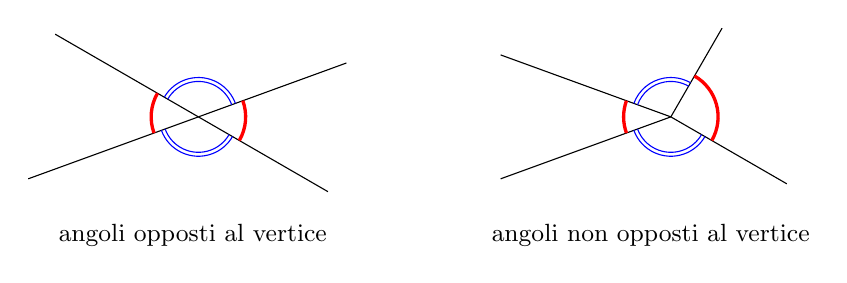
\begin{tikzpicture}
\pgfmathsetmacro{\myscale}{1};

\begin{scope}[scale={\myscale},font=\small]
\usetikzlibrary{calc}

\begin{scope}
\pgfmathsetmacro{\aalpha}{20};
\pgfmathsetmacro{\abeta}{150};
\pgfmathsetmacro{\agamma}{200};
\pgfmathsetmacro{\adelta}{330};

\coordinate (o) at (0,0);
\draw (o) -- ++({\aalpha}:2) coordinate (a);
\draw (o) -- ++({\abeta}:2.1) coordinate (b);
\draw (o) -- ++({\agamma}:2.3) coordinate (c);
\draw (o) -- ++({\adelta}:1.9) coordinate (d);

\draw[thin,blue] ([shift=({\abeta}:.45)]o) arc [radius=.45, start angle={\abeta}, end angle={\aalpha}];
\draw[thin,blue] ([shift=({\abeta}:.5)]o) arc [radius=.5, start angle={\abeta}, end angle={\aalpha}];
\draw[very thick, red] ([shift=({\agamma}:.6)]o) arc [radius =.6, start angle={\agamma}, end angle={\abeta}];
\draw[thin,blue] ([shift=({\agamma}:.45)]o) arc [radius=.45, start angle={\agamma}, end angle={\adelta}];
\draw[thin,blue] ([shift=({\agamma}:.5)]o) arc [radius=.5, start angle={\agamma}, end angle={\adelta}];
\draw[very thick, red] ([shift=({\adelta}:.6)]o) arc [radius =.6, start angle={\adelta}, end angle={360+\aalpha}];

\coordinate [label=0:angoli opposti al vertice] (l1) at (-1.9,-1.5);
\end{scope}


\pgfmathsetmacro{\myxshift}{6cm};
\begin{scope}[xshift={\myxshift}]
\pgfmathsetmacro{\aalpha}{60};
\pgfmathsetmacro{\abeta}{160};
\pgfmathsetmacro{\agamma}{200};
\pgfmathsetmacro{\adelta}{330};

\coordinate (o) at (0,0);
\draw (o) -- ++({\aalpha}:1.3) coordinate (a);
\draw (o) -- ++({\abeta}:2.3) coordinate (b);
\draw (o) -- ++({\agamma}:2.3) coordinate (c);
\draw (o) -- ++({\adelta}:1.7) coordinate (d);

\draw[thin,blue] ([shift=({\abeta}:.45)]o) arc [radius=.45, start angle={\abeta}, end angle={\aalpha}];
\draw[thin,blue] ([shift=({\abeta}:.5)]o) arc [radius=.5, start angle={\abeta}, end angle={\aalpha}];
\draw[very thick, red] ([shift=({\agamma}:.6)]o) arc [radius =.6, start angle={\agamma}, end angle={\abeta}];
\draw[thin,blue] ([shift=({\agamma}:.45)]o) arc [radius=.45, start angle={\agamma}, end angle={\adelta}];
\draw[thin,blue] ([shift=({\agamma}:.5)]o) arc [radius=.5, start angle={\agamma}, end angle={\adelta}];
\draw[very thick, red] ([shift=({\adelta}:.6)]o) arc [radius =.6, start angle={\adelta}, end angle={360+\aalpha}];

\coordinate [label=0:angoli non opposti al vertice] (l1) at (-2.4,-1.5);

\end{scope}

\end{scope}
\end{tikzpicture}

\caption{Gli angoli formati dalle semirette a sinistra sono opposti 
al vertice; gli angoli formati dalle semirette a destra non lo 
sono}\label{fig:1.24}
\end{figure}
\end{inaccessibleblock}

\vspazio\ovalbox{\risolvii \ref{ese:1.51}, \ref{ese:1.52}, 
\ref{ese:1.53}, \ref{ese:1.54}, \ref{ese:1.55}, \ref{ese:1.56}, 
\ref{ese:1.57}, \ref{ese:1.58}, \ref{ese:1.59}, \ref{ese:1.60}, 
\ref{ese:1.61}, \ref{ese:1.62}, \ref{ese:1.63},
}

\ovalbox{\ref{ese:1.64}, \ref{ese:1.65}}


\section{Confronto e operazioni tra segmenti e 
angoli}\label{sect:operazioni_segmenti_angoli}

\subsection{Premessa intuitiva}

Nel linguaggio comune usiamo la parola ``uguale'' con un significato 
generico, spesso per indicare due oggetti che si assomigliano: due 
macchine uguali, due orologi uguali,~\ldots{} In aritmetica e in 
algebra usiamo la parola ``uguale'' per indicare oggetti matematici 
perfettamente uguali. Per esempio, \(2=2\), ogni numero infatti è 
uguale solo a se stesso. Scriviamo anche \(3+2=5\), per dire che il 
numero che si ottiene dalla somma di 3 e 2 è proprio il numero 5. Nei 
polinomi si enuncia il principio di identità dei polinomi, in base al 
quale due polinomi sono uguali se si possono scrivere formalmente 
allo stesso modo.

In geometria, usiamo il termine ``uguale'' per indicare due figure 
coincidenti nella forma e nella posizione. In altre parole due figure 
sono \emph{uguali} solo se sono esattamente la stessa figura. 
Tuttavia, in geometria siamo interessati a studiare soprattutto 
figure che senza essere del tutto identiche hanno delle 
caratteristiche in comune. Vediamo prima degli esempi intuitivi e 
successivamente tratteremo lo stesso tema ma in modo formalmente 
corretto.


\begin{inaccessibleblock}[Figura: TODO]
 \begin{figure}[htb]
\centering% Copyright (c) 2015 Daniele Masini - d.masini.it@gmail.com

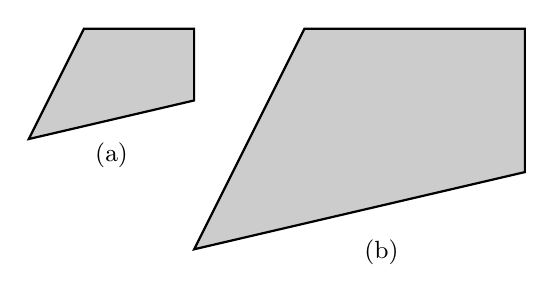
\begin{tikzpicture}[scale=.7,font=\small]
\usetikzlibrary{calc}

\begin{scope}
\coordinate (a) at (0,0);
\coordinate (b) at (1,2);
\coordinate (c) at (3,2);
\coordinate (d) at (3,0.7);
\draw[thick, fill={gray!40!white}] (a) -- (b) -- (c) -- (d) -- cycle;
\node at (1.5,-0.3) {(a)};
\end{scope}

\begin{scope}[xshift=3cm, yshift=-2cm, scale=2]
\coordinate (a) at (0,0);
\coordinate (b) at (1,2);
\coordinate (c) at (3,2);
\coordinate (d) at (3,0.7);
\draw[thick, fill={gray!40!white}] (a) -- (b) -- (c) -- (d) -- cycle;
\node at (1.7,-0.03) {(b)};
\end{scope}

\end{tikzpicture}
\qquad\qquad
% Copyright (c) 2015 Daniele Masini - d.masini.it@gmail.com

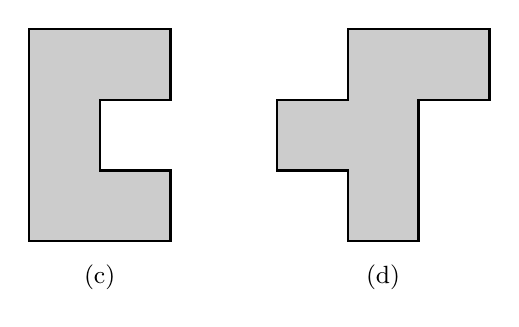
\begin{tikzpicture}[scale=.9,font=\small]
\usetikzlibrary{calc}

\begin{scope}
\coordinate (a) at (0,0);
\coordinate (b) at (2,0);
\coordinate (c) at (2,-1);
\coordinate (d) at (1,-1);
\coordinate (e) at (1,-2);
\coordinate (f) at (2,-2);
\coordinate (g) at (2,-3);
\coordinate (h) at (0,-3);
\draw[thick, fill={gray!40!white}] (a) -- (b) -- (c) -- (d) -- (e) -- (f) -- (g) -- (h) -- cycle;
\node at (1,-3.5) {(c)};
\end{scope}

\begin{scope}[xshift=3.5cm]
\coordinate (a) at (1,0);
\coordinate (b) at (3,0);
\coordinate (c) at (3,-1);
\coordinate (d) at (2,-1);
\coordinate (e) at (2,-3);
\coordinate (f) at (1,-3);
\coordinate (g) at (1,-2);
\coordinate (h) at (0,-2);
\coordinate (i) at (0,-1);
\coordinate (j) at (1,-1);
\draw[thick, fill={gray!40!white}] (a) -- (b) -- (c) -- (d) -- (e) -- (f) -- (g) -- (h) -- (i) -- (j) -- cycle;
\node at (1.5,-3.5) {(d)};
\end{scope}

\end{tikzpicture}

\end{figure}
\end{inaccessibleblock}

Le figure (a) e (b), sopra riportate, hanno la stessa forma ma una è 
più grande dell'altra, la seconda infatti è stata ottenuta dalla 
prima raddoppiando la lunghezza di ogni lato: in geometria tali 
figure si dicono \emph{simili}.

Le figure (c) e (d), invece, non hanno la stessa forma e non si 
somigliano affatto, però le loro superfici hanno la stessa 
estensione, in quanto sono costituite dallo stesso numero di 
quadratini: in geometria tali figure si dicono \emph{equivalenti}.


\begin{inaccessibleblock}[Figura: TODO]
 \begin{figure}[htb]
\centering% Copyright (c) 2015 Daniele Masini - d.masini.it@gmail.com

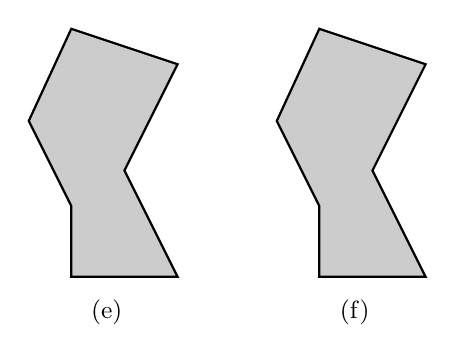
\begin{tikzpicture}[scale=.9,font=\small]
\usetikzlibrary{calc}

\begin{scope}
\coordinate (a) at (0,0);
\coordinate (b) at (1.5,-.5);
\coordinate (c) at (0.75,-2);
\coordinate (d) at (1.5,-3.5);
\coordinate (e) at (0,-3.5);
\coordinate (f) at (0,-2.5);
\coordinate (g) at (-0.6,-1.3);
\draw[thick, fill={gray!40!white}] (a) -- (b) -- (c) -- (d) -- (e) -- (f) -- (g) -- cycle;
\node at (0.5,-4) {(e)};
\end{scope}

\begin{scope}[xshift=3.5cm]
\coordinate (a) at (0,0);
\coordinate (b) at (1.5,-.5);
\coordinate (c) at (0.75,-2);
\coordinate (d) at (1.5,-3.5);
\coordinate (e) at (0,-3.5);
\coordinate (f) at (0,-2.5);
\coordinate (g) at (-0.6,-1.3);
\draw[thick, fill={gray!40!white}] (a) -- (b) -- (c) -- (d) -- (e) -- (f) -- (g) -- cycle;
\node at (0.5,-4) {(f)};
\end{scope}

\end{tikzpicture}
\qquad\qquad
% Copyright (c) 2015 Daniele Masini - d.masini.it@gmail.com

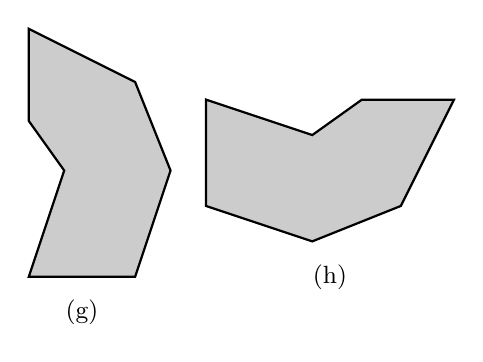
\begin{tikzpicture}[scale=.9,font=\small]
\usetikzlibrary{calc}

\begin{scope}
\coordinate (a) at (0,0);
\coordinate (b) at (1.5,-0.75);
\coordinate (c) at (2,-2);
\coordinate (d) at (1.5,-3.5);
\coordinate (e) at (0,-3.5);
\coordinate (f) at (0.5,-2);
\coordinate (g) at (0,-1.3);
\draw[thick, fill={gray!40!white}] (a) -- (b) -- (c) -- (d) -- (e) -- (f) -- (g) -- cycle;
\node at (0.75,-4) {(g)};
\end{scope}

\begin{scope}[xshift=3.5cm]
\begin{scope}[rotate=270,yshift=2.5cm, xshift=1cm]
\coordinate (a) at (0,0);
\coordinate (b) at (1.5,-0.75);
\coordinate (c) at (2,-2);
\coordinate (d) at (1.5,-3.5);
\coordinate (e) at (0,-3.5);
\coordinate (f) at (0.5,-2);
\coordinate (g) at (0,-1.3);
\draw[thick, fill={gray!40!white}] (a) -- (b) -- (c) -- (d) -- (e) -- (f) -- (g) -- cycle;
\end{scope}
\node at (0.75,-3.5) {(h)};
\end{scope}

\end{tikzpicture}

\end{figure}
\end{inaccessibleblock}

Le figure (e) ed (f) hanno la stessa forma e le stesse dimensioni ma 
sono in posizioni differenti. \`E comunque possibile spostarle una 
sull'altra e farle coincidere. Usualmente le chiamiamo figure uguali, 
ma più precisamente in geometria tali figure si dicono 
\emph{congruenti}.

Le figure (g) e (h) hanno la stessa forma e le stesse dimensioni (per 
rendersene conto basta ruotare, per esempio, la seconda figura in 
senso antiorario e poi trascinarla sulla prima per sovrapporla). 
Anche queste figure sono dette uguali nel linguaggio comune, ma in 
geometria si dicono \emph{congruenti}.

Le figure (i) e (j) hanno stessa forma e stesse dimensioni, tuttavia 
non si riesce a trasportare l'una sull'altra muovendole nel piano, né 
trascinandole, né ruotandole. Per farlo è necessario ribaltarne una 
facendola uscire dal piano, poiché le due figure sono una l'immagine 
speculare dell'altra. In geometria tali figure sono dette 
\emph{inversamente congruenti}.


\begin{inaccessibleblock}[Figura: TODO]
 \begin{figure}[htb]
\centering% Copyright (c) 2015 Daniele Masini - d.masini.it@gmail.com

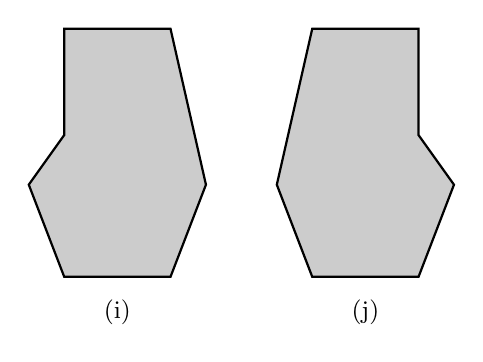
\begin{tikzpicture}[scale=.9,font=\small]
\usetikzlibrary{calc}

\begin{scope}
\coordinate (a) at (0,0);
\coordinate (b) at (1.5,0);
\coordinate (c) at (2,-2.2);
\coordinate (d) at (1.5,-3.5);
\coordinate (e) at (0,-3.5);
\coordinate (f) at (-0.5,-2.2);
\coordinate (g) at (0,-1.5);
\draw[thick, fill={gray!40!white}] (a) -- (b) -- (c) -- (d) -- (e) -- (f) -- (g) -- cycle;
\node at (0.75,-4) {(i)};
\end{scope}

\begin{scope}[xshift=5cm, xscale=-1]
\coordinate (a) at (0,0);
\coordinate (b) at (1.5,0);
\coordinate (c) at (2,-2.2);
\coordinate (d) at (1.5,-3.5);
\coordinate (e) at (0,-3.5);
\coordinate (f) at (-0.5,-2.2);
\coordinate (g) at (0,-1.5);
\draw[thick, fill={gray!40!white}] (a) -- (b) -- (c) -- (d) -- (e) -- (f) -- (g) -- cycle;
\node at (0.75,-4) {(j)};
\end{scope}

\end{tikzpicture}
\label{fig:figure_i_j}
\end{figure}
\end{inaccessibleblock}

\osservazione Per ribaltare una figura occorre una dimensione in più 
rispetto a quelle della figura, precisamente se si tratta di due 
figure piane (che hanno due dimensioni: lunghezza e larghezza)  
occorre avere la terza dimensione per effettuare un ribaltamento; se 
siamo su una retta (una sola dimensione: la lunghezza) occorre la 
seconda dimensione per ribaltare un segmento.

Per renderci conto di quanto accade con le figure solide, possiamo 
pensare ai palmi delle nostre mani che con buona approssimazione si 
possono considerare inversamente congruenti: esse possono essere 
giunte, ma non sovrapposte. Infatti non è possibile vedere le proprie 
mani sovrapposte, entrambe dal dorso o entrambe dal palmo, con le 
dita rivolte verso l'alto.

\subsection{La congruenza}

Secondo il punto di vista del matematico tedesco Felix Klein 
(1848-1925), la geometria è lo studio delle proprietà delle figure 
che sono invarianti rispetto a certe trasformazioni. Nello studio 
della geometria euclidea, quella che tratteremo in questo Tema, ci 
occupiamo delle proprietà delle figure geometriche invarianti 
rispetto ai movimenti rigidi, cioè rispetto a quei movimenti che 
conservano forma e dimensioni delle figure. Queste trasformazioni 
vengono anche dette \emph{isometrie} (si intuisce dalla radice 
etimologica che si parla di stessa misura): significa che viene 
stabilita una corrispondenza biunivoca tra i punti di due figure 
congruenti in modo da ``mantenere'' le distanze.

\begin{definizione}
Diciamo che due figure \(F\) e \(G\) sono \emph{congruenti} quando esiste 
un movimento rigido che le sovrappone perfettamente. In simboli 
\(F\cong G\).
\end{definizione}

Nella Premessa a questo paragrafo abbiamo dato un'idea intuitiva e 
sperimentale del concetto di congruenza. Ma per esplicitarlo 
matematicamente dobbiamo utilizzare gli assiomi di congruenza di 
Hilbert che abbiamo enunciato nella sezione~\ref{sect:ass_Hilbert}. 
Ne riportiamo alcuni per comodità del lettore.


\subsubsection{Assiomi di congruenza}

\begin{enumerate}[label=\Roman{*}.]
\setcounter{enumi}{2}
\item \emph{Assioma del trasporto di un segmento}. Se \(A\) e \(B\) sono 
due punti di una retta \(a\) e \(A'\) è un punto sulla stessa retta o su 
un'altra retta \(a'\), si può sempre trovare un punto \(B'\) sulla retta 
\(a\) o su \(a'\), da una data parte rispetto ad \(A'\), tale che il 
segmento \(AB\) sia congruente al segmento \(A'B'\).
\end{enumerate}
Questo assioma afferma che, fissato un punto \(A'\) su una retta \(a'\), 
è sempre possibile trasportare un qualunque segmento \(AB\) in modo che 
l'estremo \(A\) coincida con \(A'\) e il segmento stia sulla retta \(a'\).

\begin{enumerate}[label=\Roman{*}.]
\setcounter{enumi}{3}
\item La relazione di congruenza tra segmenti è \emph{transitiva}, 
cioè se \(A'B'\) e \(A''B''\) sono entrambi congruenti ad \(AB\), allora 
\(A'B'\) è congruente a \(A''B''\).
\end{enumerate}
La relazione di congruenza tra segmenti è allora un relazione di 
equivalenza, in quanto gode delle proprietà:
\begin{enumeratea}
\item \emph{riflessiva}: ogni segmento è congruente a se stesso;
\item \emph{simmetrica}: se \(AB\) è congruente a \(A'B'\) allora anche 
\(A'B'\) è congruente ad \(AB\);
\item \emph{transitiva}: se \(AB\) è congruente ad \(A'B'\) e \(A'B'\) è 
congruente ad \(A''B''\), allora \(AB\) è congruente ad \(A''B''\).
\end{enumeratea}

\begin{definizione}
Si dice \emph{lunghezza di un segmento} la classe di equivalenza dei 
segmenti congruenti tra di loro, cioè l'insieme di tutti i segmenti 
che sono congruenti tra di loro.
\end{definizione}

\begin{enumerate}[label=\Roman{*}.]
\setcounter{enumi}{4}
\item \emph{Assioma del trasporto di un angolo}. Dati un angolo 
\(A\widehat{B}C\) ed una semiretta \(B'C'\) , esistono e sono uniche due 
semirette \(B'D\) e \(B'E\), tali che l'angolo \(D\widehat{B'}C'\) risulti 
congruente all'angolo \(D\widehat{B}C\) e l'angolo \(E\widehat{B'}C'\) 
risulti congruente all'angolo \(D\widehat{B}C\).
\end{enumerate}
Questo assioma ci garantisce che è sempre possibile trasportare un 
angolo su una qualsiasi semiretta, facendo coincidere il vertice 
dell'angolo con l'origine della semiretta e un lato dell'angolo con 
la semiretta stessa.

\begin{enumerate}[label=\Roman{*}.]
\setcounter{enumi}{5}
\item La relazione di congruenza tra angoli è \emph{transitiva}, cioè 
se \(A'\widehat{B'}C'\) e \(A''\widehat{B''}C''\) sono entrambi 
congruenti ad \(A\widehat{B}C\), allora \(A'\widehat{B'}C'\) è congruente 
a \(A''\widehat{B''}C''\).
\end{enumerate}

Quindi anche la relazione di congruenza tra gli angoli è una 
relazione di equivalenza, gode cioè delle proprietà 
\emph{riflessiva}, \emph{simmetrica} e \emph{transitiva}.

\begin{definizione}
Si dice \emph{ampiezza di un angolo} la classe di equivalenza degli 
angoli congruenti tra di loro, cioè l'insieme di tutti gli angoli che 
sono congruenti tra di loro.
\end{definizione}

Aggiungiamo che:
\begin{itemize*}
\item tutte le rette sono fra loro congruenti;
\item tutte le semirette sono fra loro congruenti;
\item tutti i piani sono fra loro congruenti.
\end{itemize*}

\subsection{Confronto di segmenti}

Per confrontare l'altezza di due persone e vedere chi è più alto, le 
facciamo mettere affiancate in modo che i piedi stiano allo stesso 
livello, dopodiché confrontiamo l'estremità della testa: è più alto 
chi ha l'estremità della testa più in alto. Un procedimento analogo 
si fa per confrontare due segmenti.

Per confrontare due segmenti \(AB\) e \(CD\), facciamo in modo che con un 
movimento rigido gli estremi \(A\) e \(C\) coincidano, con una rotazione 
intorno al punto \(A\) facciamo in  modo che coincidano anche le rette 
\(AB\) e \(CD\) e che gli estremi \(B\) e \(D\) stiano dalla stessa parte 
rispetto ad \(A\) e \(C\).


\begin{inaccessibleblock}[Figura: TODO]
 \begin{figure}[htb]
\centering% Copyright (c) 2015 Daniele Masini - d.masini.it@gmail.com

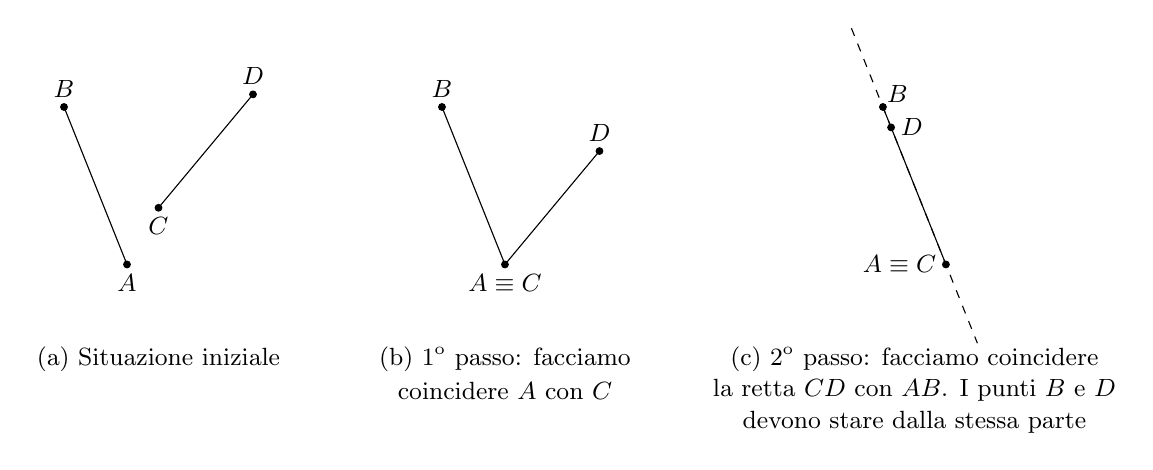
\begin{tikzpicture}[scale=.8,font=\small]
\usetikzlibrary{calc}

\begin{scope}
\coordinate (a) at (1,0);
\coordinate (b) at (0,2.5);
\coordinate (c) at (1.5,0.9);
\coordinate (d) at (3,2.7);
\draw[fill] (a) circle (1.5pt) node[below] {$A$} -- (b)circle (1.5pt) node[above] {$B$};
\draw[fill] (c) circle (1.5pt) node[below] {$C$} -- (d)circle (1.5pt) node[above] {$D$};

\node at (1.5,-1.5) {(a) Situazione iniziale};
\end{scope}

\begin{scope}[xshift=6cm]
\coordinate (a) at (1,0);
\coordinate (b) at (0,2.5);
\coordinate (c) at (1,0);
\coordinate (d) at (2.5,1.8);
\draw[fill] (a) circle (1.5pt) node[below] {$A\equiv C$} -- (b) circle (1.5pt) node[above] {$B$};
\draw[fill] (c) -- (d) circle (1.5pt) node[above] {$D$};

\node at (1,-1.5) {(b) 1\textsuperscript{o} passo: facciamo};
\node at (1,-2.0) {coincidere $A$ con $C$};
\end{scope}

\begin{scope}[xshift=13cm]
\coordinate (a) at (1,0);
\coordinate (b) at (0,2.5);
\coordinate (c) at (1,0);
%sqrt((1)^2+(2.5)^2)=2.692582404
%sqrt((1.5)^2+(1.8)^2)=2.343074903
%0.870196173
\coordinate (d) at ($(a)!0.870196173!(b)$);
\draw[dashed] ($(b)!-0.5!(a)$) -- ($(b)!1.5!(a)$);

\draw[fill] (a) circle (1.5pt) node[left] {$A\equiv C$} -- (b) circle (1.5pt) node[above right=-2pt] {$B$};
\draw[fill] (d) circle (1.5pt) node[right] {$D$};

%\draw (c) -- (d) node[above] {$D$};

\node at (0.5,-1.5) {(c) 2\textsuperscript{o} passo: facciamo coincidere};
\node at (0.5,-2) {la retta $CD$ con $AB$. I punti $B$ e $D$};
\node at (0.5,-2.5) {devono stare dalla stessa parte};
\end{scope}

\end{tikzpicture}

\caption{Confronto di due segmenti}
\end{figure}
\end{inaccessibleblock}

A questo punto sono possibili tre situazioni:
\begin{itemize*}
\item \(B\) cade dopo l'estremo \(D\), allora diciamo che \(AB\) è 
\emph{maggiore} di \(CD\) e scriviamo \(AB>CD\);
\item \(B\) cade esattamente su \(D\), allora i due segmenti sono 
\emph{congruenti} e scriviamo \(AB\cong CD\);
\item \(B\) cade tra \(C\) e \(D\), allora diciamo che \(AB\) è \emph{minore} 
di \(CD\) e scriviamo \(AB<CD\).
\end{itemize*}

\subsection{Confronto di angoli}

Per confrontare due angoli \(A\widehat{B}C\) e \(D\widehat{E}F\), 
portiamo con un movimento rigido il vertice \(B\) sul vertice \(E\), con 
una rotazione portiamo a coincidere la semiretta \(BA\) con la 
semiretta \(EF\), in modo che le altre due semirette, \(BC\) e \(ED\), 
stiano dalla stessa parte rispetto a \(BA\).


\begin{inaccessibleblock}[Figura: TODO]
 \begin{figure}[htb]
\centering% Copyright (c) 2015 Daniele Masini - d.masini.it@gmail.com

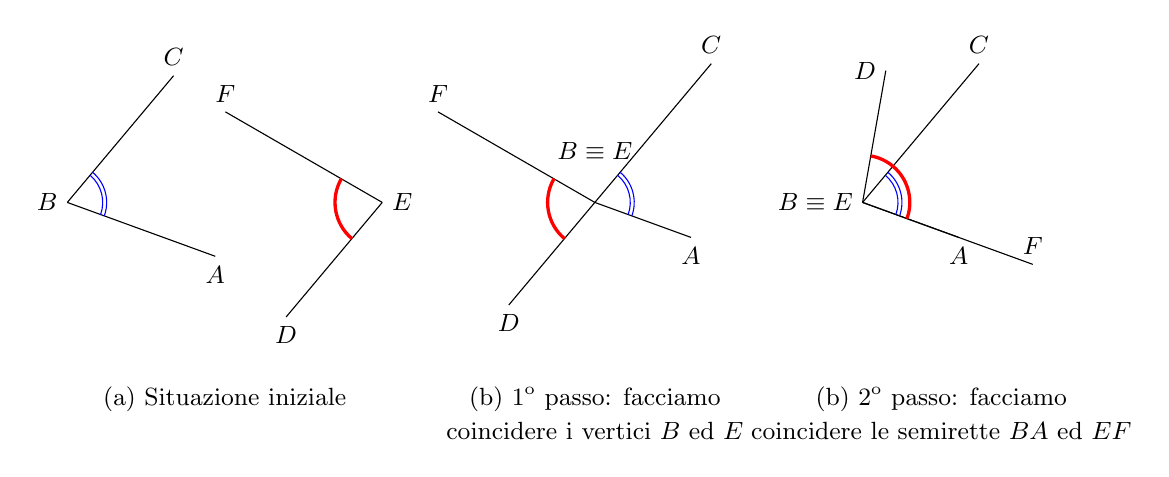
\begin{tikzpicture}
\pgfmathsetmacro{\myscale}{1};

\begin{scope}[scale={\myscale},font=\small]
\usetikzlibrary{calc}

\begin{scope}
\pgfmathsetmacro{\aalpha}{-20};
\pgfmathsetmacro{\abeta}{50};
\pgfmathsetmacro{\agamma}{150};
\pgfmathsetmacro{\adelta}{230};

\coordinate (o) at (0,0);
\coordinate (o1) at (4,0);
\draw (o) node[left] {$B$} -- ++({\aalpha}:2) coordinate (a) node[below] {$A$};
\draw (o) -- ++({\abeta}:2.1) coordinate (b) node[above] {$C$};
\draw (o1) node[right] {$E$} -- ++({\agamma}:2.3) coordinate (c) node[above] {$F$};
\draw (o1) -- ++({\adelta}:1.9) coordinate (d) node[below] {$D$};

\draw[thin,blue] ([shift=({\abeta}:.45)]o) arc [radius=.45, start angle={\abeta}, end angle={\aalpha}];
\draw[thin,blue] ([shift=({\abeta}:.5)]o) arc [radius=.5, start angle={\abeta}, end angle={\aalpha}];
\draw[very thick, red] ([shift=({\agamma}:.6)]o1) arc [radius=.6, start angle={\agamma}, end angle={\adelta}];

\node at (2,-2.5) {(a) Situazione iniziale};
\end{scope}


\begin{scope}[xshift=6.7cm]
\pgfmathsetmacro{\aalpha}{-20};
\pgfmathsetmacro{\abeta}{50};
\pgfmathsetmacro{\agamma}{150};
\pgfmathsetmacro{\adelta}{230};

\coordinate (o) at (0,0);
\draw (o) node[above=12pt] {$B\equiv E$} -- ++({\aalpha}:1.3) coordinate (a) node[below] {$A$};
\draw (o) -- ++({\abeta}:2.3) coordinate (b) node[above] {$C$};
\draw (o) -- ++({\agamma}:2.3) coordinate (c) node[above] {$F$};
\draw (o) -- ++({\adelta}:1.7) coordinate (d) node[below] {$D$};

\draw[thin,blue] ([shift=({\abeta}:.45)]o) arc [radius=.45, start angle={\abeta}, end angle={\aalpha}];
\draw[thin,blue] ([shift=({\abeta}:.5)]o) arc [radius=.5, start angle={\abeta}, end angle={\aalpha}];
\draw[very thick, red] ([shift=({\agamma}:.6)]o) arc [radius=.6, start angle={\agamma}, end angle={\adelta}];

\node at (0,-2.5) {(b) 1\textsuperscript{o} passo: facciamo};
\node at (0,-2.9) {coincidere i vertici $B$ ed $E$};

\end{scope}

\begin{scope}[xshift=10.1cm]
\pgfmathsetmacro{\aalpha}{-20};
\pgfmathsetmacro{\abeta}{50};
\pgfmathsetmacro{\agamma}{-20};
\pgfmathsetmacro{\adelta}{80};

\coordinate (o) at (0,0);
\draw (o) node[left] {$B\equiv E$} -- ++({\aalpha}:1.3) coordinate (a) node[below] {$A$};
\draw (o) -- ++({\abeta}:2.3) coordinate (b) node[above] {$C$};
\draw (o) -- ++({\agamma}:2.3) coordinate (c) node[above] {$F$};
\draw (o) -- ++({\adelta}:1.7) coordinate (d) node[left] {$D$};

\draw[thin,blue] ([shift=({\abeta}:.45)]o) arc [radius=.45, start angle={\abeta}, end angle={\aalpha}];
\draw[thin,blue] ([shift=({\abeta}:.5)]o) arc [radius=.5, start angle={\abeta}, end angle={\aalpha}];
\draw[very thick, red] ([shift=({\agamma}:.6)]o) arc [radius=.6, start angle={\agamma}, end angle={\adelta}];

\node at (1,-2.5) {(b) 2\textsuperscript{o} passo: facciamo};
\node at (1,-2.9) {coincidere le semirette $BA$ ed $EF$};

\end{scope}


\end{scope}
\end{tikzpicture}

\caption{Confronto di due angoli}
\end{figure}
\end{inaccessibleblock}

A questo punto si possono avere tre situazioni distinte:
\begin{itemize*}
\item il lato \(EF\) cade internamente all'angolo \(A\widehat{B}C\) e 
quindi diciamo che \(A\widehat{B}C\) è \emph{maggiore} di 
\(D\widehat{E}F\): \(A\widehat{B}C>D\widehat{E}F\);
\item il lato \(EF\) cade esattamente su \(BC\) e quindi i due angoli 
sono \emph{congruenti}: \(A\widehat{B}C\cong D\widehat{E}F\);
\item il lato \(EF\) cade esternamente all'angolo \(A\widehat{B}C\) e 
quindi diciamo che \(A\widehat{B}C\) è \emph{minore} di 
\(D\widehat{E}F\): \(A\widehat{B}C<D\widehat{E}F\).
\end{itemize*}

\subsection{Operazioni con i segmenti}

\paragraph{Somma di due segmenti.} La somma di due segmenti \(AB\) e 
\(CD\) è il segmento \(AD\) che si ottiene trasportando con un movimento 
rigido il segmento \(CD\) in modo che \(AB\) e \(CD\) siano adiacenti, con 
l'estremo \(B\) coincidente con \(C\). Scriviamo \(AB + CD \cong AD\), 
usando l'usuale simbolo di addizione.


\begin{inaccessibleblock}[Figura: TODO]
 \begin{figure}[htb]
\centering% Copyright (c) 2015 Daniele Masini - d.masini.it@gmail.com

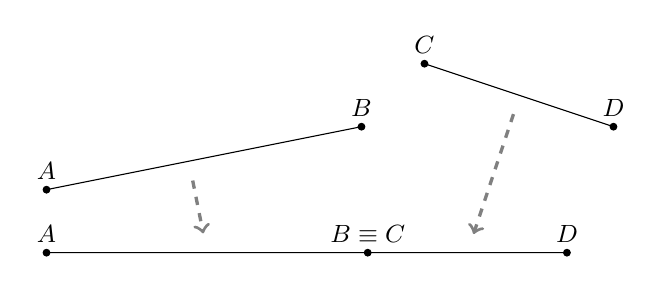
\begin{tikzpicture}[scale=0.8,font=\small,shorten line/.style={shorten >=#1,shorten <=#1}]
\usetikzlibrary{calc}

\begin{scope}
\coordinate (a) at (-1,0);
\coordinate (b) at (4,1);
\coordinate (c) at (5,2);
\coordinate (d) at (8,1);
\draw[fill] (a) circle (1.5pt) node[above] {$A$} -- (b)circle (1.5pt) node[above] {$B$};
\draw[fill] (c) circle (1.5pt) node[above] {$C$} -- (d)circle (1.5pt) node[above] {$D$};
\coordinate (a1) at (-1,-1);
\coordinate (b1) at ({sqrt((5^2)+1)-1},-1);
\coordinate (c1) at (b1);
\coordinate (d1) at ({sqrt((3^2)+1)+(sqrt((5^2)+1)-1)},-1);

\draw[fill] (a1) circle (1.5pt) node[above] {$A$} -- (b1)circle (1.5pt) node[above] {$B\equiv C$} -- (d1)circle (1.5pt) node[above] {$D$};

\coordinate (p1) at ($(a1)!0.5!(b1)$);
\coordinate (p2) at ($(c1)!0.5!(d1)$);

\draw[shorten line=0.25cm,dashed, very thick, gray,->] ($(a)!(p1)!(b)$) -- (p1);
\draw[shorten line=0.25cm,dashed, very thick, gray,->] ($(c)!(p2)!(d)$) -- (p2);
\end{scope}

\end{tikzpicture}

\caption{Somma di due segmenti. Il segmento \(AD\) è la somma dei 
segmenti \(AB\) e \(CD\)}
\end{figure}
\end{inaccessibleblock}

\paragraph{Differenza di due segmenti.} La differenza di due segmenti 
\(AB\) e \(CD\), con \(AB>CD\), è il segmento \(DB\) che si ottiene 
sovrapponendo \(AB\) e \(CD\) facendo coincidere l'estremo \(A\) con 
l'estremo \(C\). Scriviamo \(AB-CD \cong DB\).


\begin{inaccessibleblock}[Figura: TODO]
 \begin{figure}[htb]
\centering% Copyright (c) 2015 Daniele Masini - d.masini.it@gmail.com

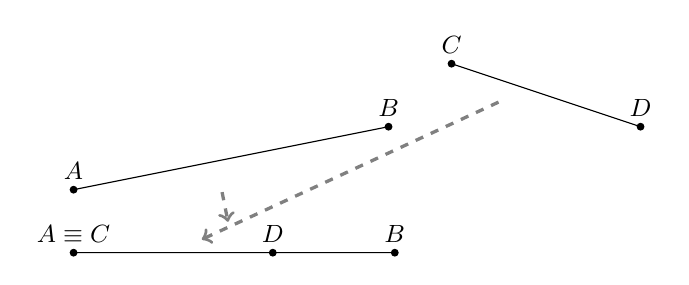
\begin{tikzpicture}[scale=0.8,font=\small,shorten line/.style={shorten >=#1,shorten <=#1}]
\usetikzlibrary{calc}

\begin{scope}
\coordinate (a) at (-1,0);
\coordinate (b) at (4,1);
\coordinate (c) at (5,2);
\coordinate (d) at (8,1);
\draw[fill] (a) circle (1.5pt) node[above] {$A$} -- (b)circle (1.5pt) node[above] {$B$};
\draw[fill] (c) circle (1.5pt) node[above] {$C$} -- (d)circle (1.5pt) node[above] {$D$};
\coordinate (a1) at (-1,-1);
\coordinate (b1) at ({sqrt((5^2)+1)-1},-1);
\coordinate (c1) at (b1);
\coordinate (d1) at ({sqrt((3^2)+1)-1)},-1);

\draw[fill] (a1) circle (1.5pt) node[above] {$A\equiv C$} -- (b1) circle (1.5pt) node[above] {$B$};
\draw[fill] (d1) circle (1.5pt) node[above] {$D$};

\coordinate (p1) at ($(a1)!0.5!(b1)$);
\coordinate (p2) at ($(a1)!0.5!(d1)$);

\draw[shorten line=0.4cm,dashed, very thick, gray,->] ($(a)!(p1)!(b)$) -- (p1);
\draw[shorten line=0.4cm,dashed, very thick, gray,->] (6.2,1.6) -- (p2);
\end{scope}

\end{tikzpicture}

\caption{Differenza di due segmenti. Il segmento \(DB\) è la differenza 
dei segmenti \(AB\) e \(CD\)}
\end{figure}
\end{inaccessibleblock}

\paragraph{Multiplo di un segmento.} Il multiplo secondo \(m\), numero 
naturale diverso da 0, di un segmento \(AB\) è il segmento \(AC\) che si 
ottiene sommando \(m\) volte il segmento \(AB\) a se stesso.


\begin{inaccessibleblock}[Figura: TODO]
 \begin{figure}[htb]
\centering% Copyright (c) 2015 Daniele Masini - d.masini.it@gmail.com

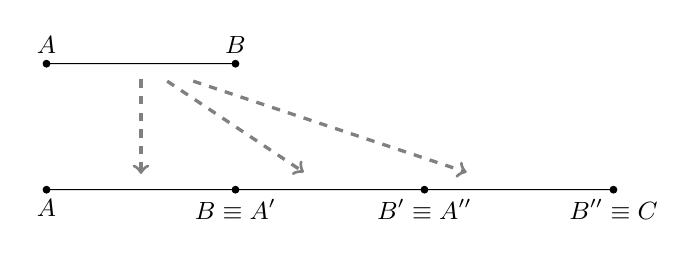
\begin{tikzpicture}[scale=0.8,font=\small,shorten line/.style={shorten >=#1,shorten <=#1}]
\usetikzlibrary{calc}

\begin{scope}
\coordinate (a) at (0,0);
\coordinate (b) at (3,0);
\draw[fill] (a) circle (1.5pt) node[above] {$A$} -- (b)circle (1.5pt) node[above] {$B$};
\coordinate (a1) at (0,-2);
\coordinate (b1) at (3,-2);
\coordinate (b2) at (6,-2);
\coordinate (b3) at (9,-2);

\draw[fill] (a1) circle (1.5pt) node[below] {$A$} -- (b1) circle (1.5pt) node[below] {$B\equiv A'$} -- (b2) circle (1.5pt) node[below] {$B'\equiv A''$} -- (b3) circle (1.5pt) node[below] {$B''\equiv C$};

\coordinate (p1) at ($(a1)!0.5!(b1)$);
\coordinate (p2) at ($(b1)!0.5!(b2)$);
\coordinate (p3) at ($(b2)!0.5!(b3)$);

\draw[shorten line=0.2cm,dashed, very thick, gray,->] ($(a)!(p1)!(b)$) -- (p1);
\draw[shorten line=0.4cm,dashed, very thick, gray,->] ($(a)!(p1)!(b)$) -- (p2);
\draw[shorten line=0.7cm,dashed, very thick, gray,->] ($(a)!(p1)!(b)$) -- (p3);
\end{scope}

\end{tikzpicture}

\caption{Multiplo di un segmento. Il segmento \(AC\) è il multiplo 
secondo 3 di \(AB\), cioè \(AC\cong 3\cdot AB\)}
\end{figure}
\end{inaccessibleblock}

Se \(m=0\), il multiplo secondo \(m\) di qualsiasi segmento \(AB\) è il 
segmento nullo, ove per segmento nullo intendiamo un qualsiasi 
segmento in cui gli estremi coincidono, cioè il segmento ridotto a un 
solo punto.

\paragraph{Sottomultiplo di un segmento.} Il sottomultiplo secondo 
\(n\), numero naturale diverso da 0, di un segmento \(AB\) è un segmento 
\(AC\) tale che \(AB\cong n\cdot AC\). Si può anche scrivere \(AC \cong 
\dfrac{1}{n}\cdot AB\).

In generale, il segmento \(AC\cong\dfrac{m}{n}\cdot AB\) si ottiene 
dividendo \(AB\) in \(n\) parti uguali ottenendo il segmento \(AD\) e poi 
sommando \(m\) segmenti congruenti ad \(AD\).


\begin{inaccessibleblock}[Figura: TODO]
 \begin{figure}[htb]
\centering% Copyright (c) 2015 Daniele Masini - d.masini.it@gmail.com

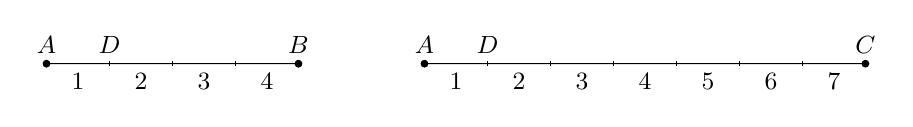
\begin{tikzpicture}[scale=0.8,font=\small,shorten line/.style={shorten >=#1,shorten <=#1}]
\usetikzlibrary{calc}

\begin{scope}
\coordinate (a) at (0,0);
\coordinate (b) at (4,0);

\foreach \x in {1,2,3,4}{%
\draw ({\x},-1pt) -- ({\x},1pt);
\node[below] at ({\x-0.5},0) {\x};
}
\draw[fill] (a) circle (1.5pt) node[above] {$A$} -- (b) circle (1.5pt) node[above] {$B$};
\node[above] at (1,0) {$D$};
\end{scope}

\begin{scope}[xshift=6cm]
\coordinate (a) at (0,0);
\coordinate (c) at (7,0);

\foreach \x in {1,2,...,7}{%
\draw ({\x},-1pt) -- ({\x},1pt);
\node[below] at ({\x-0.5},0) {\x};
}
\draw[fill] (a) circle (1.5pt) node[above] {$A$} -- (c) circle (1.5pt) node[above] {$C$};
\node[above] at (1,0) {$D$};
\end{scope}

\end{tikzpicture}

\caption{Sottomultiplo di un segmento. Il segmento \(AC\) è congruente 
a \(\dfrac{7}{4}\) di \(AB\), cioè \(AC\cong\dfrac{7}{4}\cdot AB\), infatti 
\(AB\) è stato suddiviso in 4 parti uguali e \(AC\) è costituito da 7 di 
tali parti}
\end{figure}
\end{inaccessibleblock}

\begin{definizione}
Dato un segmento \(AB\) si chiama \emph{punto medio di un segmento} il 
punto \(M\) interno al segmento che lo divide in due parti tra loro 
congruenti (\(AM\cong MB\)).
\end{definizione}


\begin{inaccessibleblock}[Figura: TODO]
 \begin{figure}[htb]
\centering% Copyright (c) 2015 Daniele Masini - d.masini.it@gmail.com

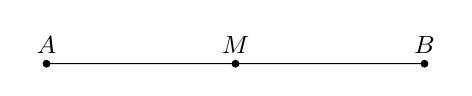
\begin{tikzpicture}[scale=0.8,font=\small,shorten line/.style={shorten >=#1,shorten <=#1}]
\usetikzlibrary{calc}
\usetikzlibrary{patterns,arrows,decorations.pathreplacing}

\begin{scope}
\coordinate (a) at (0,0);
\coordinate (b) at (6,0);
\coordinate (m) at (3,0);

\draw[fill] (a) circle (1.5pt) node[above] {$A$} -- (b) circle (1.5pt) node[above] {$B$};
\draw[fill] (m) circle (1.5pt) node[above] {$M$};
%\draw [gray,decorate,decoration={brace,amplitude=10pt,mirror},xshift=0.4pt,yshift=-0.4pt](0,-0.2) -- (3,-0.2) node[midway] {};
%\draw [gray,decorate,decoration={brace,amplitude=10pt,mirror},xshift=0.4pt,yshift=-0.4pt](3,-0.2) -- (6,-0.2) node[midway] {};
\end{scope}

\end{tikzpicture}

\caption{Punto medio di un segmento. \(M\) è il punto medio del 
segmento \(AB\) poiché \(AM\cong MB\)}
\end{figure}
\end{inaccessibleblock}

Proprietà:
\begin{itemize*}
\item somme di segmenti a due a due congruenti sono congruenti; 
\item differenze di segmenti a due a due congruenti sono congruenti.
\end{itemize*}

\begin{exrig}
\begin{esempio}
Siano \(AB\) e \(CD\) due segmenti congruenti appartenenti a una retta 
\(r\) che non abbiano punti in comune. Dimostra che \(AD-BC\cong 2\cdot 
AB\).
\begin{proof}
Disponiamo i punti \(A\), \(B\), \(C\), \(D\) su una retta \(r\) come in figura.

\begin{inaccessibleblock}[Figura: TODO]
 \begin{figure}[htb]
\centering% Copyright (c) 2015 Daniele Masini - d.masini.it@gmail.com

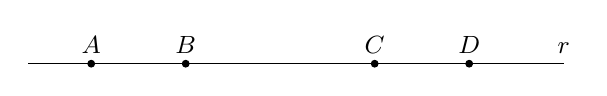
\begin{tikzpicture}[scale=0.8,font=\small,shorten line/.style={shorten >=#1,shorten <=#1}]
\usetikzlibrary{calc}
\usetikzlibrary{patterns,arrows,decorations.pathreplacing}

\begin{scope}
\coordinate (a) at (0,0);
\coordinate (b) at (6,0);
\coordinate (m) at (3,0);

\draw (-1,0) -- (7.5,0) node[above] {$r$};
\foreach \x/\y in {0/A,1.5/B,4.5/C,6/D}{%
\draw[fill] (\x,0) circle (1.5pt) node[above] {$\y$};
}
\end{scope}

\end{tikzpicture}

\end{figure}
\end{inaccessibleblock}

Per definizione di somma di segmenti si ha che \(AD\cong AB+BC+CD\) e 
quindi
\[AD-BC\cong AB+BC+CD-BC\cong AB+CD.\]
Poiché \(AB\cong CD\) si ha che
\[AD-BC\cong AB+CD\cong AB+AB\cong 2\cdot AB.\]
\end{proof}
\end{esempio}
\end{exrig}

\subsection{Operazioni con gli angoli}

\paragraph{Somma di angoli.} La somma di due angoli consecutivi 
\(A\widehat{O}B\) e \(B\widehat{O}C\) è l'angolo \(A\widehat{O}C\). Per 
sommare due angoli che non sono consecutivi, per esempio 
\(A\widehat{B}C\) e \(D\widehat{E}F\), si costruiscono due angoli 
consecutivi tra di loro, uno congruente a \(A\widehat{B}C\), l'altro 
congruente a \(D\widehat{E}F\) e quindi si calcola la somma 
(figura~\ref{fig:1.32}).


\begin{inaccessibleblock}[Figura: TODO]
 \begin{figure}[htb]
\centering% Copyright (c) 2015 Daniele Masini - d.masini.it@gmail.com

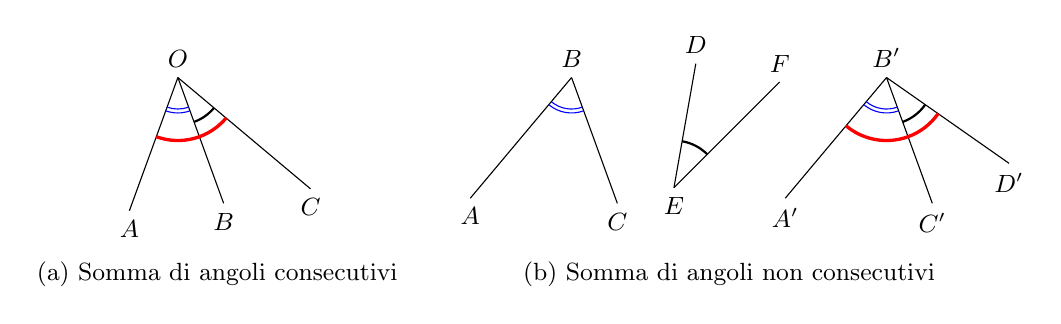
\begin{tikzpicture}
\pgfmathsetmacro{\myscale}{1};

\begin{scope}[scale={\myscale},font=\small]
\usetikzlibrary{calc}

\begin{scope}
\pgfmathsetmacro{\aalpha}{250};
\pgfmathsetmacro{\abeta}{290};
\pgfmathsetmacro{\agamma}{320};

\coordinate (o) at (0,0);
\draw (o) node[above] {$O$} -- ++({\aalpha}:1.8) coordinate (a) node[below] {$A$};
\draw (o) -- ++({\abeta}:1.7) coordinate (b) node[below] {$B$};
\draw (o) -- ++({\agamma}:2.2) coordinate (c) node[below] {$C$};

\draw[thin,blue] ([shift=({\abeta}:.4)]o) arc [radius=.4, start angle={\abeta}, end angle={\aalpha}];
\draw[thin,blue] ([shift=({\abeta}:.45)]o) arc [radius=.45, start angle={\abeta}, end angle={\aalpha}];
\draw[thick, black] ([shift=({\abeta}:.6)]o) arc [radius=.6, start angle={\abeta}, end angle={\agamma}];
\draw[very thick, red] ([shift=({\aalpha}:.8)]o) arc [radius=.8, start angle={\aalpha}, end angle={\agamma}];

\node at (0.5,-2.5) {(a) Somma di angoli consecutivi};
\end{scope}


\begin{scope}[xshift=5cm]
\pgfmathsetmacro{\aalpha}{230};
\pgfmathsetmacro{\abeta}{290};
\pgfmathsetmacro{\agamma}{80};
\pgfmathsetmacro{\adelta}{45};

\coordinate (o) at (0,0);
\coordinate (o1) at (1.3,-1.4);
\draw (o) node[above] {$B$} -- ++({\aalpha}:2) coordinate (a) node[below] {$A$};
\draw (o) -- ++({\abeta}:1.7) coordinate (b) node[below] {$C$};
\draw (o1) node[below] {$E$} -- ++({\agamma}:1.6) coordinate (c) node[above] {$D$};
\draw (o1) -- ++({\adelta}:1.9) coordinate (d) node[above] {$F$};

\draw[thin,blue] ([shift=({\abeta}:.4)]o) arc [radius=.4, start angle={\abeta}, end angle={\aalpha}];
\draw[thin,blue] ([shift=({\abeta}:.45)]o) arc [radius=.45, start angle={\abeta}, end angle={\aalpha}];
\draw[thick, black] ([shift=({\agamma}:.6)]o1) arc [radius=.6, start angle={\agamma}, end angle={\adelta}];
\end{scope}

\begin{scope}[xshift=9cm]
\pgfmathsetmacro{\aalpha}{230};
\pgfmathsetmacro{\abeta}{290};
\pgfmathsetmacro{\agamma}{325};

\coordinate (o) at (0,0);
\draw (o) node[above] {$B'$} -- ++({\aalpha}:2) coordinate (a) node[below] {$A'$};
\draw (o) -- ++({\abeta}:1.7) coordinate (b) node[below] {$C'$};
\draw (o) -- ++({\agamma}:1.9) coordinate (c) node[below] {$D'$};

\draw[thin,blue] ([shift=({\abeta}:.4)]o) arc [radius=.4, start angle={\abeta}, end angle={\aalpha}];
\draw[thin,blue] ([shift=({\abeta}:.45)]o) arc [radius=.45, start angle={\abeta}, end angle={\aalpha}];
\draw[thick, black] ([shift=({\abeta}:.6)]o) arc [radius=.6, start angle={\abeta}, end angle={\agamma}];
\draw[very thick, red] ([shift=({\aalpha}:.8)]o) arc [radius=.8, start angle={\aalpha}, end angle={\agamma}];

\node at (-2,-2.5) {(b) Somma di angoli non consecutivi};
\end{scope}

\end{scope}
\end{tikzpicture}

\caption{Somma di due angoli.}\label{fig:1.32}
\end{figure}
\end{inaccessibleblock}

\paragraph{Differenza di angoli.} La differenza di due angoli, di cui 
il primo è maggiore o congruente al secondo, è l'angolo che 
addizionato al secondo dà per somma il primo (figura~\ref{fig:1.33}). 
Se i due angoli considerati sono congruenti la loro differenza è 
l'angolo nullo.


\begin{inaccessibleblock}[Figura: TODO]
 \begin{figure}[htb]
\centering% Copyright (c) 2015 Daniele Masini - d.masini.it@gmail.com

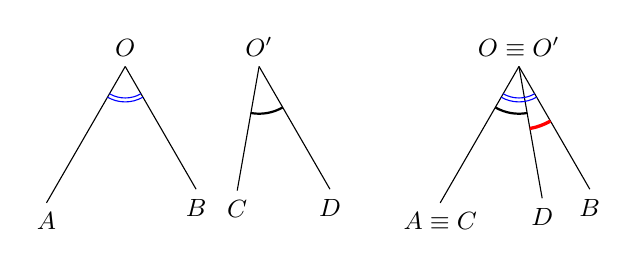
\begin{tikzpicture}
\pgfmathsetmacro{\myscale}{1};

\begin{scope}[scale={\myscale},font=\small]
\usetikzlibrary{calc}

\begin{scope}
\pgfmathsetmacro{\aalpha}{240};
\pgfmathsetmacro{\abeta}{300};
\pgfmathsetmacro{\agamma}{260};
\pgfmathsetmacro{\adelta}{300};

\coordinate (o) at (0,0);
\coordinate (o1) at (1.7,0);
\draw (o) node[above] {$O$} -- ++({\aalpha}:2) coordinate (a) node[below] {$A$};
\draw (o) -- ++({\abeta}:1.8) coordinate (b) node[below] {$B$};
\draw (o1) node[above] {$O'$} -- ++({\agamma}:1.6) coordinate (c) node[below] {$C$};
\draw (o1) -- ++({\adelta}:1.8) coordinate (d) node[below] {$D$};

\draw[thin,blue] ([shift=({\abeta}:.4)]o) arc [radius=.4, start angle={\abeta}, end angle={\aalpha}];
\draw[thin,blue] ([shift=({\abeta}:.45)]o) arc [radius=.45, start angle={\abeta}, end angle={\aalpha}];
\draw[thick, black] ([shift=({\agamma}:.6)]o1) arc [radius=.6, start angle={\agamma}, end angle={\adelta}];
\end{scope}

\begin{scope}[xshift=5cm]
\pgfmathsetmacro{\aalpha}{240};
\pgfmathsetmacro{\abeta}{300};
\pgfmathsetmacro{\agamma}{280};

\coordinate (o) at (0,0);
\draw (o) node[above] {$O\equiv O'$} -- ++({\aalpha}:2) coordinate (a) node[below] {$A\equiv C$};
\draw (o) -- ++({\abeta}:1.8) coordinate (b) node[below] {$B$};
\draw (o) -- ++({\agamma}:1.7) coordinate (c) node[below] {$D$};

\draw[thin,blue] ([shift=({\abeta}:.4)]o) arc [radius=.4, start angle={\abeta}, end angle={\aalpha}];
\draw[thin,blue] ([shift=({\abeta}:.45)]o) arc [radius=.45, start angle={\abeta}, end angle={\aalpha}];
\draw[thick, black] ([shift=({\aalpha}:.6)]o) arc [radius=.6, start angle={\aalpha}, end angle={\agamma}];
\draw[very thick, red] ([shift=({\agamma}:.8)]o) arc [radius=.8, start angle={\agamma}, end angle={\abeta}];
\end{scope}

\end{scope}
\end{tikzpicture}

\caption{Differenza di due angoli.}\label{fig:1.33}
\end{figure}
\end{inaccessibleblock}

\paragraph{Multiplo di un angolo.} Dato un angolo \(A\widehat{O}B\) e 
un numero \(n\) naturale non nullo, il multiplo di \(A\widehat{O}B\) 
secondo \(n\) (si può scrivere \(n\cdot A\widehat{O}B\)) è l'angolo che 
si ottiene sommando \(n\) angoli congruenti a \(A\widehat{O}B\). Se 
\(n=0\), il multiplo secondo \(n\) di qualsiasi angolo \(A\widehat{O}B\) è 
l'angolo nullo.


\begin{inaccessibleblock}[Figura: TODO]
 \begin{figure}[htb]
\centering% Copyright (c) 2015 Daniele Masini - d.masini.it@gmail.com

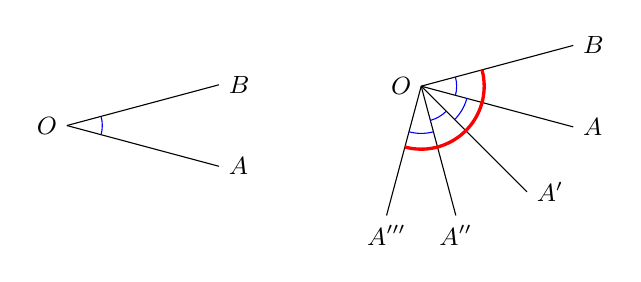
\begin{tikzpicture}
\pgfmathsetmacro{\myscale}{1};

\begin{scope}[scale={\myscale},font=\small]
\usetikzlibrary{calc}

\begin{scope}
\pgfmathsetmacro{\aalpha}{-15};
\pgfmathsetmacro{\abeta}{15};

\coordinate (o) at (0,0);
\draw (o) node[left] {$O$} -- ++({\aalpha}:2) coordinate (a) node[right] {$A$};
\draw (o) -- ++({\abeta}:2) coordinate (b) node[right] {$B$};

\draw[blue] ([shift=({\abeta}:.45)]o) arc [radius=.45, start angle={\abeta}, end angle={\aalpha}];
\end{scope}

\begin{scope}[xshift=4.5cm, yshift=0.5cm]
\pgfmathsetmacro{\aalpha}{15};
\pgfmathsetmacro{\abeta}{-15};
\pgfmathsetmacro{\agamma}{-45};
\pgfmathsetmacro{\adelta}{-75};
\pgfmathsetmacro{\aepsilon}{-105};

\coordinate (o) at (0,0);
\draw (o) node[left] {$O$} -- ++({\aalpha}:2) coordinate (a) node[right] {$B$};
\draw (o) -- ++({\abeta}:2) coordinate (b) node[right] {$A$};
\draw (o) -- ++({\agamma}:1.9) coordinate (c) node[right] {$A'$};
\draw (o) -- ++({\adelta}:1.7) coordinate (d) node[below] {$A''$};
\draw (o) -- ++({\aepsilon}:1.7) coordinate (e) node[below] {$A'''$};

\draw[blue] ([shift=({\abeta}:.45)]o) arc [radius=.45, start angle={\abeta}, end angle={\aalpha}];
\draw[blue] ([shift=({\agamma}:.6)]o) arc [radius=.6, start angle={\agamma}, end angle={\abeta}];
\draw[blue] ([shift=({\adelta}:.45)]o) arc [radius=.45, start angle={\adelta}, end angle={\agamma}];
\draw[blue] ([shift=({\aepsilon}:.6)]o) arc [radius=.6, start angle={\aepsilon}, end angle={\adelta}];

\draw[very thick, red] ([shift=({\aepsilon}:.8)]o) arc [radius=.8, start angle={\aepsilon}, end angle={\aalpha}];
\end{scope}

\end{scope}
\end{tikzpicture}

\caption{Multiplo di un angolo. L'angolo \(A'''\widehat{O}B\) è il 
quadruplo di \(A\widehat{O}B\), cioè \(A'''\widehat{O}B \cong 4\cdot 
A\widehat{O}B\)}
\end{figure}
\end{inaccessibleblock}

\paragraph{Sottomultiplo di un angolo.} Il sottomultiplo secondo \(n\), 
naturale non nullo, di un angolo \(A\widehat{O}B\) è un angolo 
\(A\widehat{O}C\) tale che \(A\widehat{O}B \cong n\cdot A\widehat{O}C\). 
Si può anche scrivere \(A\widehat{O}C\cong \dfrac{1}{n}\cdot 
A\widehat{O}B\).

In generale, un angolo \(A\widehat{O}C\cong\dfrac{m}{n}\cdot 
A\widehat{O}B\) si ottiene suddividendo \(A\widehat{O}B\) in \(n\) angoli 
uguali (indichiamo con \(A\widehat{O}D\) il primo di essi), quindi 
l'angolo \(A\widehat{O}C\) è ottenuto sommando \(m\) volte l'angolo 
\(A\widehat{O}D\).

\begin{definizione}
Si dice \emph{bisettrice di un angolo} la semiretta che ha origine 
nel vertice dell'angolo e che lo divide in due angoli tra loro 
congruenti.
\end{definizione}


\begin{inaccessibleblock}[Figura: TODO]
 \begin{figure}[htb]
\centering% Copyright (c) 2015 Daniele Masini - d.masini.it@gmail.com

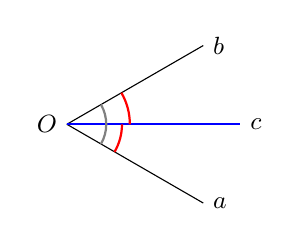
\begin{tikzpicture}
\pgfmathsetmacro{\myscale}{1};

\begin{scope}[scale={\myscale},font=\small]
\usetikzlibrary{calc}

\begin{scope}
\pgfmathsetmacro{\aalpha}{-30};
\pgfmathsetmacro{\abeta}{30};
\pgfmathsetmacro{\agamma}{0};


\coordinate (o) at (0,0);
\draw (o) node[left] {$O$} -- ++({\aalpha}:2) coordinate (a) node[right] {$a$};
\draw (o) -- ++({\abeta}:2) coordinate (b) node[right] {$b$};
\draw[blue, thick] (o) -- ++({\agamma}:2.2) coordinate (b) node[right,black] {$c$};

\draw[thick,gray] ([shift=({\aalpha}:.5)]o) arc [radius=.5, start angle={\aalpha}, end angle={\abeta}];
\draw[thick,red] ([shift=({\abeta}:.8)]o) arc [radius=.8, start angle={\abeta}, end angle={\agamma}];
\draw[thick,red] ([shift=({\agamma}:.7)]o) arc [radius=.7, start angle={\agamma}, end angle={\aalpha}];
\end{scope}

\end{scope}
\end{tikzpicture}

\caption{La semiretta \(c\) è la bisettrice dell'angolo 
\(a\widehat{O}b\), gli angoli \(a\widehat{O}c\) e \(c\widehat{O}b\) sono 
congruenti}
\end{figure}
\end{inaccessibleblock}

\subsection{Angoli particolari}

Possiamo ora dare dei nomi ai seguenti angoli particolari.

\begin{definizione}
Si dice \emph{angolo retto} la metà di un angolo piatto.
\end{definizione}

Per denotare il fatto che un angolo è retto si è soliti indicarlo con 
un quadratino al posto dell'usuale archetto.


\begin{inaccessibleblock}[Figura: TODO]
 \begin{figure}[htb]
\centering% Copyright (c) 2015 Daniele Masini - d.masini.it@gmail.com

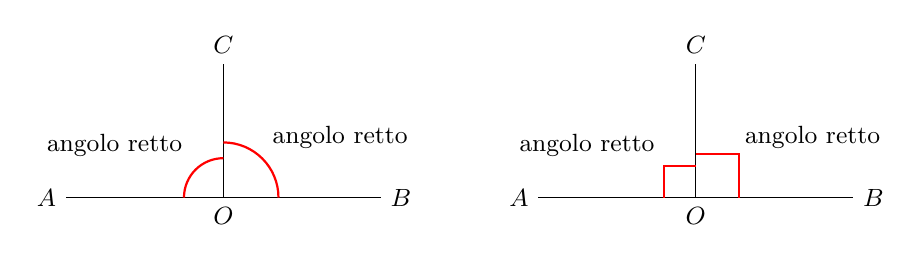
\begin{tikzpicture}
\pgfmathsetmacro{\myscale}{1};

\begin{scope}[scale={\myscale},font=\small]
\usetikzlibrary{calc}

\begin{scope}
\pgfmathsetmacro{\aalpha}{180};
\pgfmathsetmacro{\abeta}{0};
\pgfmathsetmacro{\agamma}{90};


\coordinate (o) at (0,0);
\draw (o) node[below] {$O$} -- ++({\aalpha}:2) coordinate (a) node[left] {$A$};
\draw (o) -- ++({\abeta}:2) coordinate (b) node[right] {$B$};
\draw (o) -- ++({\agamma}:1.7) coordinate (b) node[above] {$C$};

\draw[thick,red] ([shift=({\abeta}:.7)]o) arc [radius=.7, start angle={\abeta}, end angle={\agamma}];
\draw[thick,red] ([shift=({\agamma}:.5)]o) arc [radius=.5, start angle={\agamma}, end angle={\aalpha}];
\node[above right] at (.5,.5) {angolo retto};
\node[above left] at (-.4,.4) {angolo retto};
\end{scope}


\begin{scope}[xshift=6cm]
\pgfmathsetmacro{\aalpha}{180};
\pgfmathsetmacro{\abeta}{0};
\pgfmathsetmacro{\agamma}{90};


\coordinate (o) at (0,0);
\draw (o) node[below] {$O$} -- ++({\aalpha}:2) coordinate (a) node[left] {$A$};
\draw (o) -- ++({\abeta}:2) coordinate (b) node[right] {$B$};
\draw (o) -- ++({\agamma}:1.7) coordinate (b) node[above] {$C$};

\draw[thick,red] (.55,0) -- (.55,.55) --(0,.55);
\draw[thick,red] (-.4,0) -- (-.4,.4) --(0,.4);
\node[above right] at (.5,.5) {angolo retto};
\node[above left] at (-.4,.4) {angolo retto};
\end{scope}


\end{scope}
\end{tikzpicture}

\end{figure}
\end{inaccessibleblock}

\begin{definizione}
Due angoli si dicono \emph{complementari} se la loro somma è un 
angolo retto.
\end{definizione}


\begin{inaccessibleblock}[Figura: TODO]
 \begin{figure}[htb]
\centering% Copyright (c) 2015 Daniele Masini - d.masini.it@gmail.com

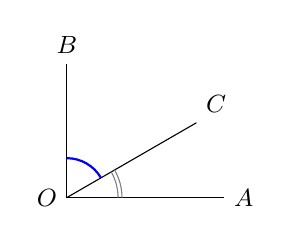
\begin{tikzpicture}
\pgfmathsetmacro{\myscale}{1};

\begin{scope}[scale={\myscale},font=\small]
\usetikzlibrary{calc}

\begin{scope}
\pgfmathsetmacro{\aalpha}{0};
\pgfmathsetmacro{\abeta}{90};
\pgfmathsetmacro{\agamma}{30};


\coordinate (o) at (0,0);
\draw (o) node[left] {$O$} -- ++({\aalpha}:2) coordinate (a) node[right] {$A$};
\draw (o) -- ++({\abeta}:1.7) coordinate (b) node[above] {$B$};
\draw (o) -- ++({\agamma}:1.9) coordinate (b) node[above right] {$C$};

\draw[thick,blue] ([shift=({\abeta}:.5)]o) arc [radius=.5, start angle={\abeta}, end angle={\agamma}];
\draw[gray] ([shift=({\agamma}:.65)]o) arc [radius=.65, start angle={\agamma}, end angle={\aalpha}];
\draw[gray] ([shift=({\agamma}:.70)]o) arc [radius=.70, start angle={\agamma}, end angle={\aalpha}];
\end{scope}

\end{scope}
\end{tikzpicture}

\end{figure}
\end{inaccessibleblock}

\begin{definizione}
Due angoli si dicono \emph{supplementari} se la loro somma è un 
angolo piatto.
\end{definizione}


\begin{inaccessibleblock}[Figura: TODO]
 \begin{figure}[htb]
\centering% Copyright (c) 2015 Daniele Masini - d.masini.it@gmail.com

\begin{tikzpicture}
\pgfmathsetmacro{\myscale}{1};

\begin{scope}[scale={\myscale},font=\small]
\usetikzlibrary{calc}

\begin{scope}
\pgfmathsetmacro{\aalpha}{0};
\pgfmathsetmacro{\abeta}{180};
\pgfmathsetmacro{\agamma}{45};


\coordinate (o) at (0,0);
\draw (o) node[below] {$O$} -- ++({\aalpha}:2) coordinate (a) node[right] {$A$};
\draw (o) -- ++({\abeta}:2) coordinate (b) node[left] {$B$};
\draw (o) -- ++({\agamma}:1.7) coordinate (b) node[above right] {$C$};

\draw[thick,blue] ([shift=({\abeta}:.5)]o) arc [radius=.5, start angle={\abeta}, end angle={\agamma}];
\draw[gray] ([shift=({\agamma}:.65)]o) arc [radius=.65, start angle={\agamma}, end angle={\aalpha}];
\draw[gray] ([shift=({\agamma}:.70)]o) arc [radius=.70, start angle={\agamma}, end angle={\aalpha}];
\end{scope}

\end{scope}
\end{tikzpicture}

\end{figure}
\end{inaccessibleblock}

\begin{definizione}
Due angoli si dicono \emph{esplementari} se la loro somma è un angolo 
giro.
\end{definizione}


\begin{inaccessibleblock}[Figura: TODO]
 \begin{figure}[htb]
\centering% Copyright (c) 2015 Daniele Masini - d.masini.it@gmail.com

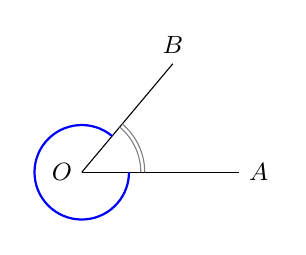
\begin{tikzpicture}
\pgfmathsetmacro{\myscale}{1};

\begin{scope}[scale={\myscale},font=\small]
\usetikzlibrary{calc}

\begin{scope}
\pgfmathsetmacro{\aalpha}{0};
\pgfmathsetmacro{\abeta}{50};


\coordinate (o) at (0,0);
\draw (o) node[left] {$O$} -- ++({\aalpha}:2) coordinate (a) node[right] {$A$};
\draw (o) -- ++({\abeta}:1.8) coordinate (b) node[above] {$B$};

\draw[thick,blue] ([shift=({\abeta}:.6)]o) arc [radius=.6, start angle={\abeta}, end angle={\aalpha+360}];
\draw[gray] ([shift=({\aalpha}:.75)]o) arc [radius=.75, start angle={\aalpha}, end angle={\abeta}];
\draw[gray] ([shift=({\aalpha}:.80)]o) arc [radius=.80, start angle={\aalpha}, end angle={\abeta}];
\end{scope}

\end{scope}
\end{tikzpicture}

\end{figure}
\end{inaccessibleblock}

\begin{definizione}
Un angolo si dice \emph{acuto} se è minore di un angolo retto.
\end{definizione}

\begin{definizione}
Un angolo convesso si dice \emph{ottuso} se è maggiore di un angolo 
retto.
\end{definizione}


\begin{inaccessibleblock}[Figura: TODO]
 \begin{figure}[htb]
\centering% Copyright (c) 2015 Daniele Masini - d.masini.it@gmail.com

\begin{tikzpicture}
\pgfmathsetmacro{\myscale}{1};

\begin{scope}[scale={\myscale},font=\small]
\usetikzlibrary{calc}

\begin{scope}
\pgfmathsetmacro{\aalpha}{0};
\pgfmathsetmacro{\abeta}{60};
\pgfmathsetmacro{\agamma}{90};

\coordinate (o) at (0,0);
\draw (o) node[below] {$O$} -- ++({\aalpha}:2) coordinate (a) node[right] {$A$};
\draw (o) -- ++({\abeta}:1.7) coordinate (b) node[above right] {$B$};
\draw[dotted,gray] (o) -- ++({\agamma}:1.7) coordinate (c);

\draw[thin,blue] ([shift=({\abeta}:.5)]o) arc [radius=.5, start angle={\abeta}, end angle={\aalpha}];
\draw[thin,blue] ([shift=({\abeta}:.55)]o) arc [radius=.55, start angle={\abeta}, end angle={\aalpha}];

\node at (1,-1) {(a) Angolo acuto};
\end{scope}

\begin{scope}[xshift=5cm]
\pgfmathsetmacro{\aalpha}{0};
\pgfmathsetmacro{\abeta}{120};
\pgfmathsetmacro{\agamma}{90};

\coordinate (o) at (0,0);
\draw (o) node[below] {$O$} -- ++({\aalpha}:2) coordinate (a) node[right] {$A$};
\draw (o) -- ++({\abeta}:1.7) coordinate (b) node[above left] {$B$};
\draw[dotted,gray] (o) -- ++({\agamma}:1.7) coordinate (c);

\draw[thin,blue] ([shift=({\abeta}:.5)]o) arc [radius=.5, start angle={\abeta}, end angle={\aalpha}];
\draw[thin,blue] ([shift=({\abeta}:.55)]o) arc [radius=.55, start angle={\abeta}, end angle={\aalpha}];

\node at (0.5,-1) {(b) Angolo ottuso};
\end{scope}

\end{scope}
\end{tikzpicture}

\end{figure}
\end{inaccessibleblock}

\begin{teorema}
Angoli opposti al vertice sono congruenti.
\end{teorema}

\begin{proof}
Si considerino due generici angoli opposti al vertice \(A\widehat{O}B\) 
e \(C\widehat{O}D\) come nella figura seguente.

\begin{inaccessibleblock}[Figura: TODO]
 \begin{figure}[htb]
\centering% Copyright (c) 2015 Daniele Masini - d.masini.it@gmail.com

\begin{tikzpicture}
\pgfmathsetmacro{\myscale}{1};

\begin{scope}[scale={\myscale},font=\small]
\usetikzlibrary{calc}

\begin{scope}
\pgfmathsetmacro{\aalpha}{30};
\pgfmathsetmacro{\abeta}{150};
\pgfmathsetmacro{\agamma}{210};
\pgfmathsetmacro{\adelta}{330};

\coordinate (o) at (0,0);
\draw (o) node[above] {$O$} -- ++({\aalpha}:2) coordinate (a) node[right] {$A$};
\draw (o) -- ++({\abeta}:2) coordinate (b) node[left] {$D$};
\draw (o) -- ++({\agamma}:2) coordinate (c) node[left] {$C$};
\draw (o) -- ++({\adelta}:2) coordinate (d) node[right] {$B$};

%\draw[thin,blue] ([shift=({\abeta}:.45)]o) arc [radius=.45, start angle={\abeta}, end angle={\aalpha}];
%\draw[thin,blue] ([shift=({\abeta}:.5)]o) arc [radius=.5, start angle={\abeta}, end angle={\aalpha}];
\draw[very thick, red] ([shift=({\agamma}:.8)]o) arc [radius =.8, start angle={\agamma}, end angle={\abeta}];
%\draw[thin,blue] ([shift=({\agamma}:.45)]o) arc [radius=.45, start angle={\agamma}, end angle={\adelta}];
%\draw[thin,blue] ([shift=({\agamma}:.5)]o) arc [radius=.5, start angle={\agamma}, end angle={\adelta}];
\draw[very thick, red] ([shift=({\adelta}:.8)]o) arc [radius =.8, start angle={\adelta}, end angle={360+\aalpha}];
\end{scope}

\end{scope}
\end{tikzpicture}

\end{figure}
\end{inaccessibleblock}
Gli angoli \(A\widehat{O}B\) e \(A\widehat{O}D\) sono adiacenti, dato che 
hanno un lato in comune e gli altri due lati sono l'uno il 
prolungamento dell'altro. Ma anche gli angoli \(A\widehat{O}D\) e 
\(D\widehat{O}C\) sono angoli adiacenti per lo stesso motivo. Quindi 
gli angoli \(D\widehat{O}C\) e \(A\widehat{O}B\) sono adiacenti allo 
stesso angolo \(A\widehat{O}D\).
Indicando con \(\pi\) l'angolo piatto si ha: \(A\widehat{O}D + 
D\widehat{O}C \cong \pi\) da cui \(D\widehat{O}C\cong \pi - 
A\widehat{O}D\). Analogamente \(A\widehat{O}B+A\widehat{O}D\cong\pi\) da 
cui \(A\widehat{O}B\cong \pi-A\widehat{O}D\). Ne consegue che 
\(D\widehat{O}C\cong A\widehat{O}B\) e cioè la tesi.
\end{proof}

Prova tu a dimostrare il seguente teorema

\begin{teorema}
Angoli supplementari di angoli congruenti sono congruenti.
\end{teorema}

\emph{Suggerimento: Dopo aver realizzato il disegno, esplicita 
ipotesi e tesi. Segui poi il ragionamento del teorema precedente: se 
due angoli sono supplementari la loro somma è un angolo piatto 
\ldots{}}

\subsection{Perpendicolari e altre definizioni}

\begin{definizione}
Due rette si dicono \emph{perpendicolari} se sono incidenti e formano 
tra loro quattro angoli retti.
\end{definizione}


\begin{inaccessibleblock}[Figura: TODO]
 \begin{figure}[htb]
\centering% Copyright (c) 2015 Daniele Masini - d.masini.it@gmail.com

\begin{tikzpicture}
\pgfmathsetmacro{\myscale}{1};

\begin{scope}[scale={\myscale},font=\small]
\usetikzlibrary{calc}

\begin{scope}
\draw[thick] (-2.5,0) -- (2.5,0) node[above] {$r$};
\draw[thick] (0,1.5) node[right] {$s$} -- (0,-1.5);

\draw[red] (.55,0) -- (.55,.55) --(0,.55);
\draw[red] (-.4,0) -- (-.4,.4) --(0,.4);
\draw[red] (.4,0) -- (.4,-.4) --(0,-.4);
\draw[red] (-.55,0) -- (-.55,-.55) --(0,-.55);
\end{scope}


\end{scope}
\end{tikzpicture}

\caption{Le rette \(r\) e \(s\) sono perpendicolari poiché incontrandosi 
formano quattro angoli retti}
\end{figure}
\end{inaccessibleblock}

Per indicare che le due rette \(r\) e \(s\) sono perpendicolari si usa il 
simbolo \(r\perp s\).

\begin{definizione}
Si dice \emph{distanza di un punto \(P\) da una retta} la lunghezza del 
segmento di perpendicolare condotta dal punto \(P\) alla retta.
\end{definizione}


\begin{inaccessibleblock}[Figura: TODO]
 \begin{figure}[htb]
\centering% Copyright (c) 2015 Daniele Masini - d.masini.it@gmail.com

\begin{tikzpicture}[scale=1,font=\small]
\usetikzlibrary{calc}

\begin{scope}[rotate=20]
\draw[thick] (-2,0) -- (3,0) node[above] {$r$};
\draw[blue] (0,1.3) -- (0,0);
\path[fill] (0,1.3) circle (1.5pt) node[above] {$P$} -- (0,0) circle (1.5pt) node[below] {$H$};

\draw[red] (.55,0) -- (.55,.55) --(0,.55);
\draw[red] (-.4,0) -- (-.4,.4) --(0,.4);
\end{scope}

\end{tikzpicture}

\caption{Il segmento \(PH\), appartenente alla perpendicolare a \(r\) 
passante per \(P\), è la distanza di \(P\) dalla retta \(r\)}
\end{figure}
\end{inaccessibleblock}

\begin{definizione}\label{def:asse_segmento}
Si chiama \emph{asse di un segmento} la retta perpendicolare al 
segmento e passante per il suo punto medio.
\end{definizione}

In genere un asse viene rappresentato con una linea a ``tratto e 
punto''.


\begin{inaccessibleblock}[Figura: TODO]
 \begin{figure}[htb]
\centering% Copyright (c) 2015 Daniele Masini - d.masini.it@gmail.com

\begin{tikzpicture}
\pgfmathsetmacro{\myscale}{1};

\begin{scope}[scale={\myscale},font=\small]
\usetikzlibrary{calc}

\begin{scope}
\draw[thick,fill] (-1.5,0) circle (1.5pt) node[above] {$A$} -- (1.5,0) circle (1.5pt) node[above] {$B$};
\draw[fill] (0,0) circle (1.5pt) node[above right] {$M$};
\draw[blue,thick,dashdotted] (0,1.3) node[black,right] {$r$} -- (0,-1.3);

\draw[red] (.55,0) -- (.55,.55) --(0,.55);
\draw[red] (-.4,0) -- (-.4,.4) --(0,.4);
\draw[red] (.4,0) -- (.4,-.4) --(0,-.4);
\draw[red] (-.55,0) -- (-.55,-.55) --(0,-.55);
\end{scope}


\end{scope}
\end{tikzpicture}

\caption{La retta \(r\) è l'asse del segmento \(AB\) in quanto è 
perpendicolare alla retta per \(AB\) e passa per \(M\), il punto medio di 
\(AB\)}\label{fig:1.38}
\end{figure}
\end{inaccessibleblock}

\begin{definizione}
Due punti si dicono \emph{simmetrici rispetto a una retta} se la 
retta è asse del segmento che ha per estremi i due punti.
\end{definizione}

Nella figura~\ref{fig:1.38}, i punti \(A\) e \(B\) sono simmetrici 
rispetto alla retta \(r\).

\vspazio\ovalbox{\risolvii \ref{ese:1.66}, \ref{ese:1.67}, 
\ref{ese:1.68}, \ref{ese:1.69}, \ref{ese:1.70}, \ref{ese:1.71}, 
\ref{ese:1.72}, \ref{ese:1.73}, \ref{ese:1.74}, \ref{ese:1.75}, 
\ref{ese:1.76}, \ref{ese:1.77}, \ref{ese:1.78},}

\ovalbox{\ref{ese:1.79}, \ref{ese:1.80}, \ref{ese:1.81}, 
\ref{ese:1.82}, \ref{ese:1.83}, \ref{ese:1.84}, \ref{ese:1.85}, 
\ref{ese:1.86}, \ref{ese:1.87}, \ref{ese:1.88}, \ref{ese:1.89}, 
\ref{ese:1.90}, \ref{ese:1.91}, \ref{ese:1.92},\ref{ese:1.93}, 
\ref{ese:1.94}, \ref{ese:1.95},}

\ovalbox{\ref{ese:1.96}, \ref{ese:1.97}, \ref{ese:1.98}, 
\ref{ese:1.99}, \ref{ese:1.100}, \ref{ese:1.101}, \ref{ese:1.102}, 
\ref{ese:1.103}}


\section{La misura}\label{sect:misura}

\subsection{Misura di segmenti}

Riprendiamo alcune definizioni sui segmenti.

Si dice \emph{segmento} di estremi \(A\) e \(B\) (o brevemente 
\emph{segmento} \(AB\)) l'insieme dei punti \(A\) e \(B\) e di tutti quelli 
che stanno tra \(A\) e \(B\).
Due segmenti \(AB\) e \(CD\) si dicono \emph{congruenti} se esiste un 
movimento rigido che porta a coincidere \(A\) con \(C\) e \(B\) con \(D\), 
oppure \(A\) con \(D\) e \(B\) con \(C\). Ricordiamo che se esiste un 
movimento rigido che porta a coincidere \(A\) con \(C\) e \(B\) con \(D\) 
allora esiste anche un movimento rigido che porta a coincidere \(A\) 
con \(D\) e \(B\) con \(C\), e viceversa.

Si dice \emph{lunghezza di un segmento} \(AB\) l'insieme di tutti i 
segmenti congruenti ad \(AB\).

Si dice \emph{distanza tra due punti} \(A\) e \(B\) il segmento \(AB\) di 
estremi \(A\) e \(B\).

Diamo ora una definizione particolarmente importante per 
l'applicazione del calcolo numerico alla geometria: la definizione di 
\emph{misura}. Ricordiamo che la nozione di misura è alla base delle 
applicazioni del calcolo matematico non solo alla geometria ma anche 
alla fisica e alla tecnologia in generale. Il processo di misurazione 
è analogo a tutti i campi di applicazioni: si tratta di trovare un 
modo per assegnare a una grandezza un numero. Questo numero si 
ottiene confrontando due grandezze dello stesso tipo. Per esempio, 
per misurare la massa di un oggetto si confronta la sua massa con 
quella di un oggetto campione, di solito un oggetto di 1 kg.

Per misurare un segmento \(AB\) si confronta questo segmento con un 
altro segmento scelto come unità di misura, di solito indicato con 
\(u\).

Nel confronto tra il segmento \(AB\) e il segmento \(u\), possono 
verificarsi i tre casi seguenti:
\begin{enumerate}
\item (figura~\ref{fig:mis_segm1}) Il segmento \(AB\) è multiplo del 
segmento \(u\) secondo il numero naturale \(n\), precisamente \(AB\cong 
n\cdot u\). In questo caso la misura di \(AB\), rispetto a \(u\), è il 
numero naturale \(n\). Si scrive \(\overline{AB} = nu\).


\begin{inaccessibleblock}[Figura: TODO]
 \begin{figure}[htb]
\centering% Copyright (c) 2015 Daniele Masini - d.masini.it@gmail.com

\begin{tikzpicture}[scale=1.5,font=\small,shorten line/.style={shorten >=#1,shorten <=#1}]
\usetikzlibrary{calc}
\usetikzlibrary{patterns,arrows,decorations.pathreplacing}

\begin{scope}
\draw (0,0) -- node[above] {$u$} (1,0);
\draw (0,-1pt) -- (0,1pt);
\draw (1,-1pt) -- (1,1pt);
\end{scope}

\begin{scope}[xshift=2cm]
\draw[thick] (0,0) -- (5,0);
\foreach \x in {1,2,...,5}{
	\draw (\x,-1pt) -- (\x,1pt);
    \draw [gray,decorate,decoration={brace,amplitude=10pt,mirror},xshift=0.4pt,yshift=-0.4pt]({\x-1},-0.1) -- (\x,-0.1) node[black,below=10pt,midway] {$u$};

}
\draw[fill] (0,0) circle (1pt) node[above] {$A$};
\draw[fill] (5,0) circle (1pt) node[above] {$B$};

\end{scope}

\end{tikzpicture}

\caption{Il segmento \(AB\) misura \(5u\), cioè \(AB\cong 6\cdot u\), cioè 
\(\overline{AB}=6u\)}\label{fig:mis_segm1}
\end{figure}
\end{inaccessibleblock}

\item (figura~\ref{fig:mis_segm2}) Il segmento \(AB\) non è un multiplo 
intero di \(u\) ma è un multiplo di un sottomultiplo di \(u\), 
precisamente \(AB\cong n\cdot \dfrac{u}{m}=\dfrac{n}{m}u\). In questo 
caso la misura di \(AB\), rispetto a \(u\), è il numero razionale 
\(\dfrac{n}{m}\). Si scrive \(\overline{AB} = \dfrac{n}{m}u\).


\begin{inaccessibleblock}[Figura: TODO]
 \begin{figure}[htb]
\centering% Copyright (c) 2015 Daniele Masini - d.masini.it@gmail.com

\begin{tikzpicture}[scale=2,font=\small,shorten line/.style={shorten >=#1,shorten <=#1}]
\usetikzlibrary{calc}
\usetikzlibrary{patterns,arrows,decorations.pathreplacing}

\begin{scope}
\draw (0,0) -- node[above] {$u$} (1,0);
\draw (0,-1pt) -- (0,1pt);
\draw (1,-1pt) -- (1,1pt);

\foreach \x in {0.2,0.4,...,0.8}{
	\draw (\x,-1pt) -- (\x,0pt);
}

\draw (0,0) -- node[below=15pt] {$\frac{1}{5}u$} (0.2,0);
\draw[shorten line=0.2cm,dotted, very thick, gray,->] (0.1,-.38) -- (0.1,0);
\end{scope}

\begin{scope}[xshift=2cm]
\draw[thick] (0,0) -- (2.6,0);
\foreach \x in {0.2,0.4,...,2.4}{
	\draw (\x,-1pt) -- (\x,0pt);
}
\foreach \x in {1,2}{
	\draw (\x,0pt) -- (\x,1pt);
}

\draw[fill] (0,0) circle (0.7pt) node[above] {$A$};
\draw[fill] (2.6,0) circle (0.7pt) node[above] {$B$};

\draw [gray,decorate,decoration={brace,amplitude=10pt,mirror},xshift=0.4pt,yshift=-0.4pt](0,-0.1) -- (1,-0.1) node[black,below=10pt,midway] {$u$};
\draw [gray,decorate,decoration={brace,amplitude=10pt,mirror},xshift=0.4pt,yshift=-0.4pt](1,-0.1) -- (2,-0.1) node[black,below=10pt,midway] {$u$};
\draw [gray,decorate,decoration={brace,amplitude=10pt,mirror},xshift=0.4pt,yshift=-0.4pt](2,-0.1) -- (2.6,-0.1) node[black,below=10pt,midway] {$\frac{3}{5}u$};

\end{scope}

\end{tikzpicture}

\caption{Il segmento \(AB\) è congruente a 13 volte il segmento 
\(\dfrac{1}{5}u\), quindi \(AB\) misura \(\dfrac{13}{5}u\), cioè 
\(\overline{AB}=\dfrac{13}{5}u\)}\label{fig:mis_segm2}
\end{figure}
\end{inaccessibleblock}

\item Il segmento \(AB\) non è un multiplo né di \(u\) né di un suo 
sottomultiplo. In questo caso si dice che \(AB\) e \(u\) sono 
\emph{incommensurabili} (nei casi precedenti si dice invece che sono 
\emph{commensurabili}). Anche in questo caso è possibile attribuire 
ad \(AB\) un numero che ne esprime la misura rispetto a \(u\), si tratta 
però di un numero irrazionale. La complessità dell'argomento richiede 
alcune conoscenze più avanzate di matematica, pertanto la tematica 
della misura delle grandezze incommensurabili sarà approfondita nel 
seguito. Qui ci limitiamo ad accennare al caso storicamente più noto 
di segmenti incommensurabili: la diagonale di un quadrato misurata 
rispetto al suo lato.


\begin{inaccessibleblock}[Figura: TODO]
 \begin{figure}[htb]
\centering% Copyright (c) 2015 Daniele Masini - d.masini.it@gmail.com

\begin{tikzpicture}[scale=2,font=\small,shorten line/.style={shorten >=#1,shorten <=#1}]
\usetikzlibrary{calc}

\begin{scope}
\draw (0,0) rectangle (1,1);
\draw[blue] (0,0) -- node[black, above, midway, sloped] {$d$} (1,1);
\path (0,0) -- node[black, below, midway, sloped] {$u$} (1,0);
\path (1,0) -- node[black, right, midway] {$u$} (1,1);

\end{scope}

\end{tikzpicture}

\caption{Prendendo come unità di misura il lato di un quadrato, la 
sua diagonale è incommensurabile con il lato stesso. Applicando il 
teorema di Pitagora, ricorderai infatti che \(d=\sqrt{2}u\) e che 
\(\sqrt{2}\) è un numero irrazionale}
\end{figure}
\end{inaccessibleblock}

Proponiamo una dimostrazione dell'irrazionalità del numero \(\sqrt{2}\) 
utilizzando il metodo della dimostrazione per assurdo.

%\begin{teorema}
%\(\sqrt{2}\) è un numero irrazionale.
%\end{teorema}

\begin{proof}
Supponiamo per assurdo che \(\sqrt{2}\) sia un numero razionale, cioè 
che sia possibile scrivere \(\sqrt{2}=\dfrac{m}{n}\), con \(m,n \in 
\N\) e \(n\neq 0\). Allora, per definizione di radice quadrata, si 
avrebbe \(2=\dfrac{m^2}{n^2}\), da cui \(2n^2=m^2\). I due membri 
dovrebbero quindi rappresentare lo stesso numero naturale (il teorema 
fondamentale dell'Aritmetica assicura l'unicità della scomposizione 
in fattori primi). Essendo 2 un numero primo, dovrebbe comparire come 
fattore sia al primo sia al secondo membro lo stesso numero di volte. 
Inoltre \(m^2\) ed \(n^2\) o sono dispari e quindi se contengono il 
fattore 2 lo contengono un numero pari di volte (vediamo qualche 
esempio \(24=2^3\cdot3 \rightarrow 24^2=2^6\cdot3^2\), \(20=2^2\cdot5 
\rightarrow 20^2=2^4\cdot5^2\)). Ma \(2n^2\) contiene il fattore 2 un 
numero dispari di volte, mentre \(m^2\) lo contiene un numero pari. 
Pertanto l'uguaglianza \(2n^2=m^2\) non può essere mai verificata; 
l'assurdo deriva dall'aver supposto \(\sqrt{2}\) razionale.
\end{proof}

Un altro esempio di numero irrazionale, e di conseguenza di due 
``lunghezze'' incommensurabili, è \(\pi\), che rappresenta il rapporto 
tra la misura della lunghezza di una circonferenza e la misura della 
lunghezza del suo diametro.
\end{enumerate}

In generale, dato un segmento \(AB\) e un segmento \(u\), preso come 
unità di misura, esiste sempre un numero reale positivo che esprime 
la misura di \(AB\) rispetto a \(u\). Questo numero è unico, ossia ogni 
segmento ha una sola misura. Viceversa, dato un qualsiasi numero 
reale positivo \(r\) e un segmento \(u\), preso come unità di misura, è 
sempre possibile costruire un segmento che misura esattamente \(r\) 
rispetto all'unità di misura \(u\) fissata.

Osservazioni
\begin{itemize*}
\item Se due segmenti sono congruenti, le loro misure, rispetto alla 
stessa unità di misura, sono uguali (e viceversa): \(AB\cong CD 
\:\Leftrightarrow\: \overline{AB}=\overline{CD}\).
\item La misura di un segmento \(AB\) somma di due segmenti \(CD\) e \(EF\) 
(\(AB\cong CD + EF\)) è uguale alla somma delle misure di \(CD\) e \(EF\): 
\(AB\cong CD + EF \:\Leftrightarrow\: 
\overline{AB}=\overline{CD}+\overline{EF}\).
\item La misura di un segmento multiplo secondo \(n\) del segmento \(AB\) 
è uguale al prodotto di \(n\) per la misura di \(AB\): \(CD\cong n\cdot AB 
\:\Leftrightarrow\: \overline{CD}=n\overline{AB}\).
\item Definito il \emph{rapporto tra due segmenti} come il quoziente 
tra le loro misure \(\dfrac{CD}{AB} = 
\dfrac{\overline{CD}}{\overline{AB}}\) (rispetto alla stessa unità di 
misura), si ha che esso non dipende dall'unità di misura usata per 
misurare i segmenti, cioè il numero che si ottiene è sempre lo stesso 
indipendentemente dall'unità scelta per misurare.
\end{itemize*}

Possiamo pertanto parlare di misura della lunghezza di un segmento e 
darne la seguente definizione generale.

\begin{definizione}
Dato un segmento \(AB\) e un segmento \(u\) preso come unità di misura, 
si dice \emph{misura della lunghezza del segmento} \(AB\) il numero 
reale positivo \(r\) per il quale risulta \(AB\cong r\cdot u\).
\end{definizione}

Nella realtà fisica per misurare la lunghezza degli oggetti reali 
(l'altezza di una persona, la lunghezza di un banco, di una stanza, 
di un terreno, \ldots{}) si usa come unità di misura il metro, 
indicato con la lettera m, con i suoi  multipli (decametro, 
ettometro, chilometro, \ldots{}) e i suoi sottomultipli (decimetro, 
centimetro, millimetro, \ldots{}). Anche nella geometria, che tratta 
di segmenti ideali non riscontrabili perfettamente nella realtà, si 
usa come unità di misura un segmento di un metro.

Riassumendo, ricordiamo simboli e nozioni che riguardano due punti 
\(A\) e \(B\).
\begin{itemize*}
\item Due punti presi singolarmente con notazione insiemistica si 
indicano con \(A\) e \(B\).
\item La retta passante per i due punti si indica con il simbolo  
\(AB\) oppure \(r(A,B)\).
\item La semiretta di origine \(A\) e passante per \(B\) si indica con il 
simbolo \(AB\) oppure \(r(A,B)\).
\item Il segmento di estremi \(A\) e \(B\) si indica con il simbolo \(AB\).
\item La distanza tra i punti \(A\) e \(B\), cioè il segmento \(AB\), si 
indica con il simbolo \(AB\) oppure \(d(A,B)\).
\item La lunghezza del segmento \(AB\), cioè l'insieme di tutti i 
segmenti congruenti ad \(AB\), si indica con il simbolo \(\overline{AB}\).
\item La misura della lunghezza del segmento \(AB\) rispetto a una 
fissata unità di misura si indica con il simbolo \(\overline{AB}\).
\item La misura della distanza tra i punti \(A\) e \(B\), che corrisponde 
alla misura del segmento \(AB\), si indica con il simbolo 
\(\overline{AB}\).
\end{itemize*}

Tutte queste distinzioni sono importanti dal punto di vista 
dell'organizzazione teorica della geometria, tuttavia dal punto di 
vista applicativo e della quotidianità del linguaggio geometrico 
possono risultare pedanti e noiose, spesso si usano espressioni più 
generiche, finché si riescono ad evitare possibili malintesi. Sebbene 
a rigore si dovrebbe dire ``la misura della lunghezza del segmento 
\(AB\) rispetto al centimetro è 12'' molto spesso si usa dire ``il 
segmento \(AB\) è lungo 12~cm'' oppure ``\(AB\) misura 12~cm'' o ancora 
``la distanza tra \(A\) e \(B\) è 12~cm'' o più semplicemente ``il 
segmento \(AB\) di 12~cm'', ecc.

\subsection{Misura di angoli}

Il procedimento che si usa per misurare gli angoli è del tutto 
analogo a quello usato per misurare i segmenti. Si fissa un'unità di 
misura, cioè un angolo \(\widehat{u}\), e quindi si confronta l'angolo 
da misurare con \(\widehat{u}\). Come risultato si avrà un numero reale 
positivo che chiamiamo \emph{misura dell'ampiezza dell'angolo}.


\begin{inaccessibleblock}[Figura: TODO]
 \begin{figure}[htb]
\centering% Copyright (c) 2015 Daniele Masini - d.masini.it@gmail.com

\begin{tikzpicture}[scale=1,font=\small]
\usetikzlibrary{calc} %, angles}

\begin{scope}
\pgfmathsetmacro{\aalpha}{0};
\pgfmathsetmacro{\abeta}{20};

\coordinate (o) at (0,0);

\draw (o) -- ({\aalpha}:2.5);
\draw (o) -- ({\abeta}:2.5);

\node[right] at ({(\aalpha+\abeta)/2}:2) {$\widehat{u}$};

\draw[thick,blue] ([shift=({\aalpha}:.65)]o) arc [radius=.65, start angle={\aalpha}, end angle={\abeta}];
\end{scope}

\begin{scope}[xshift=4cm]
\pgfmathsetmacro{\aalpha}{0};
\pgfmathsetmacro{\abeta}{20};
\pgfmathsetmacro{\agamma}{40};
\pgfmathsetmacro{\adelta}{60};
\pgfmathsetmacro{\aepsilon}{80};

\coordinate (o) at (0,0);

\draw[thick] (o) node[left] {$O$} -- ({\aalpha}:2.5) node[below] {$A$};
\draw[dashed] (o) -- ({\abeta}:2.5);
\draw[dashed] (o) -- ({\agamma}:2.5);
\draw[dashed] (o) -- ({\adelta}:2.5);
\draw[thick] (o) -- ({\aepsilon}:2.5) node[left] {$B$};

\node at ({(\aalpha+\abeta)/2}:2.1) {$\widehat{u}$};
\node at ({(\abeta+\agamma)/2}:2.1) {$\widehat{u}$};
\node at ({(\agamma+\adelta)/2}:2.1) {$\widehat{u}$};
\node at ({(\adelta+\aepsilon)/2}:2.1) {$\widehat{u}$};

\draw[thick,blue] ([shift=({\aalpha}:.5)]o) arc [radius=.5, start angle={\aalpha}, end angle={\aepsilon}];
\end{scope}

\end{tikzpicture}

\caption{L'angolo \(A\widehat{O}B\) misura 4 volte l'angolo unitario 
\(\widehat{u}\)}
\end{figure}
\end{inaccessibleblock}

Per misurare gli angoli, l'unità di misura comunemente usata è la 
trecentosessantesima parte dell'angolo giro, detta \emph{grado}, e 
viene indicata con un cerchietto posto in alto (\(\grado\)) di seguito 
al numero che ne esprime la misura. Si ha quindi, usando come unità 
di misura il grado, che:
\begin{itemize*}
\item l'angolo retto misura 90 gradi e si scrive \(90\grado\);
\item l'angolo piatto misura \(180\grado\);
\item l'angolo giro misura \(360\grado\).
\end{itemize*}

I sottomultipli del grado sono il \emph{primo} (minuto primo) che è 
la sessantesima parte di un grado (in simboli \(1\grado=60'\)) e il 
\emph{secondo} (minuto secondo) che è la sessantesima parte del primo 
(in simboli \(1'=60''\)) e quindi la tremilaseicentesima parte del 
grado (in simboli \(1\grado=\np{3600}''\)).

\begin{exrig}
\begin{esempio}
Calcola la misura in gradi del supplementare dell'angolo che misura 
\(35\grado 15' 40''\).
Occorre eseguire la sottrazione \(180\grado - 35\grado 15' 40''\). Per 
eseguire praticamente questa sottrazione si trasforma \(1\grado\) in 
\(60'\) e \(1'\) in \(60''\), precisamente si scrive \(180\grado\) come 
\(179\grado 59' 60''\), pertanto:

\begin{center}
\begin{tabular}{r@{\extracolsep{2pt}}l}
\(179\grado 59' 60''\) & \(-\)\\
\(35\grado 15' 40''\) & \(=\)\\
\hline
\(144\grado 44' 20''\) & \\
\end{tabular}
\end{center}

Quindi \(180\grado - 35\grado 15' 40'' = 144\grado 44' 20''\).
\end{esempio}
\end{exrig}

Il sistema di misura degli angoli che abbiamo illustrato prende il 
nome di \emph{sistema sessagesimale}. Spesso, però, per praticità, 
anziché usare i primi, i secondi e i decimi di secondo, si usano i 
decimi di grado: in questo caso il sistema si dice \emph{sistema 
sessadecimale}.

In base a quanto descritto, vediamo brevemente come si passa da un 
sistema all'altro.

\begin{itemize}
\item \(10\grado 42' 23''\np{,2} = 
10+\dfrac{42}{60}+\dfrac{\np{23,2}}{3600} = 
10\grado\np{,706}\overline{4}\);
\item \(50\grado\np{,748} = 50\grado + (\np{0,748}\cdot 60)'=50\grado 
+ 44'\np{,88} = 50\grado + 44'+(\np{0,88}\cdot 60)'' = 50\grado 44' 
52''\np{,8}\).
\end{itemize}

I sistemi sessagesimale e sessadecimale non sono gli unici usati per 
le misure degli angoli.

Osservando i tasti di una calcolatrice scientifica, si può vedere che 
ci sono tre sistemi principali le cui unità sono rispettivamente il 
\emph{grado sessagesimale}\footnote{in realtà quasi tutte le 
calcolatrici utilizzano la notazione sessadecimale.} (DEG) che 
abbiamo precedentemente illustrato, il \emph{grado centesimale} 
(GRAD) e il \emph{radiante} (RAD).

Il grado centesimale è importante per gli strumenti tecnici. Si può 
passare dal grado sessagesimale al grado centesimale e viceversa con 
una semplice proporzione, sapendo che l'angolo retto, pari a 
\(90\grado\), corrisponde a 100 gradi centesimali (in simboli 
100\textsuperscript{g}).

Il radiante è utile nello studio della trigonometria e dell'analisi 
matematica. L'angolo di misura 1~radiante (in simboli 
1~rad\footnote{in genere l'unità di misura rad viene omessa.}) è 
congruente ad un angolo con vertice nel centro di una circonferenza e 
tale che la misura dell'arco da esso individuato è uguale alla misura 
del raggio della circonferenza stessa.
Facendo riferimento alla figura~\ref{fig:radiante}, l'angolo~\(\alpha\) 
formato dalle semirette~\(ON\) e~\(OM\) misura 1~radiante se l'arco \(MN\) 
misura quanto il raggio della circonferenza (\(\overline{OM}\)). Come 
si può facilmente intuire, il radiante ed il grado sono grandezze 
incommensurabili.


\begin{inaccessibleblock}[Figura: TODO]
 \begin{figure}[htb]
\centering% Copyright (c) 2015 Daniele Masini - d.masini.it@gmail.com

\begin{tikzpicture}
\pgfmathsetmacro{\myscale}{1};

\begin{scope}[scale={\myscale},font=\small]
\usetikzlibrary{calc}

\begin{scope}
\pgfmathsetmacro{\aalpha}{0};
\pgfmathsetmacro{\abeta}{{180/pi}};


\coordinate (o) at (0,0);
\draw (o) circle (1.5);
\draw (o) node[left] {$O$} -- ({\aalpha}:2.5) node[right] {$s$};
\draw (o) -- ({\abeta}:2.5) node[right] {$r$};

\node[below] at ({\aalpha}:1.7) {$M$};
\node[above] at ({\abeta+5}:1.5) {$N$};
\draw[thick,red] ([shift=(0:.45)]o) arc [radius=.45, start angle={\aalpha}, end angle={\abeta}];
\node at ({(\aalpha+\abeta)/2}:.65) {$\alpha$};
%\node at ({(\aalpha+\abeta)/2}:1.75) {$A$};

\draw[very thick,blue] ([shift=(0:1.5)]o) arc [radius=1.5, start angle={\aalpha}, end angle={\abeta}];
\end{scope}

\end{scope}
\end{tikzpicture}

\caption{L'angolo con ampiezza di 1 radiante}\label{fig:radiante}
\end{figure}
\end{inaccessibleblock}

\begin{osservazione}
La misura di un arco va fatta con una modalità differente rispetto a 
quella utilizzata per la misura dei segmenti. Si può immaginare di 
utilizzare come strumento di misura un metro flessibile, ovvero un 
filo flessibile ma inestensibile, che si può piegare ma non si può 
allungare o accorciare, su cui siano state tracciate, a distanza 
regolare, delle tacche corrispondenti a sottomultipli dell'unità di 
misura delle lunghezze; una di queste tacche viene assunta come 
origine del metro. Facendo combaciare l'origine del metro flessibile 
con il punto~\(M\) e flettendo il metro in modo che si sovrapponga 
all'arco~\(MN\) si otterrà la sua lunghezza.
\end{osservazione}

Ricordando che il rapporto tra la misura della circonferenza ed il 
raggio vale~\(2\pi\), dove \(\pi\) è il numero 
irrazionale~\(3,1415\ldots{}\) (i puntini indicano che la parte 
decimale è infinita e non periodica), possiamo intuire che il valore 
dell'angolo giro (\(360\grado\)), corrispondente ad un arco che 
coincide con l'intera circonferenza, vale \(2\pi\)~radianti.

Visto che un angolo giro corrisponde a \(2\pi\)~radianti, l'angolo 
piatto (\(180\grado\)) corrisponderà a \(\pi\)~radianti, quindi per 
convertire le ampiezze degli angoli da gradi a radianti e viceversa è 
sufficiente impostare la seguente proporzione:
\[180\grado : \pi = \alpha\grado : \alpha\]
dove con \(\alpha\grado\) abbiamo indicato l'ampiezza dell'angolo in 
gradi e con \(\alpha\) la sua ampiezza in radianti. Da cui si ottiene

\[\alpha\grado = 
\dfrac{180\grado}{\pi}\alpha\qquad\text{e}\qquad\alpha = 
\dfrac{\pi}{180\grado}\alpha\grado\]

Quindi, avendo un angolo espresso in radianti, per convertirlo in 
gradi si può utilizzare la prima formula inserendo al posto di 
\(\alpha\) la sua effettiva misura in radianti, mentre se abbiamo un 
angolo espresso in gradi e lo vogliamo trasformare in radianti si può 
utilizzare la seconda formula inserendo al posto di \(\alpha\grado\) 
l'effettiva misura dell'angolo in gradi.

Possiamo pertanto calcolare la misura in gradi di un angolo di 
1~radiante ponendo nella prima formula \(\alpha=1\). Si ottiene così 
\(\alpha\grado = 180\grado/\pi \simeq 57\grado\np{,297469362} \simeq 
57\grado 17'51''\).

Riportiamo di seguito una tabella che fornisce i valori degli angoli 
più comuni espressi sia in gradi che in radianti.

\begin{center}
\begin{tabular}{cc}
\toprule
angolo in gradi	& angolo in radianti\\
\midrule
\(360\grado\) & \(2\pi\)\\
\(270\grado\) & \(3\pi/2\)\\
\(180\grado\) & \(\pi\)\\
\(90\grado\) & \(\pi/2\)\\
\(60\grado\) & \(\pi/3\)\\
\(45\grado\) & \(\pi/4\)\\
\(30\grado\) & \(\pi/6\)\\
\bottomrule
\end{tabular}
\end{center}

\subsubsection{Angoli negativi}

Nei paragrafi precedenti abbiamo definito l'angolo come l'insieme dei 
punti compresi tra due semirette aventi la stessa origine \(O\). 
Possiamo però definire l'angolo anche come rotazione di una semiretta 
intorno alla propria origine, la misura di un angolo diventa allora 
la misura dell'entità della rotazione.


\begin{inaccessibleblock}[Figura: TODO]
 \begin{figure}[!htb]
	\centering% Copyright (c) 2015 Daniele Masini - d.masini.it@gmail.com

\begin{tikzpicture}
\pgfmathsetmacro{\myscale}{1};

\begin{scope}[scale={\myscale},font=\small]
\usetikzlibrary{calc}

\begin{scope}
\pgfmathsetmacro{\aalpha}{0};
\pgfmathsetmacro{\abeta}{60};


\coordinate (o) at (0,0);
\draw[dotted, blue] (o) circle (.7);
\draw (o) node[left] {$O$} -- (2.5,0) node[right] {$A$};
\draw (o) -- (60:2.5) node[right] {$B$};

\draw[very thick,blue,->] ([shift=(0:.7)]o) arc [radius=.7, start angle={\aalpha}, end angle={\abeta}];
\end{scope}

\end{scope}
\end{tikzpicture}

	\caption{Il verso positivo nella misura degli angoli è quello 
antiorario}\label{fig:1.43}
\end{figure}
\end{inaccessibleblock}

Dal momento che una rotazione può essere effettuata in due versi, 
orario o antiorario, si assume uno dei due versi di rotazione come 
positivo e l'altro negativo. Per motivi storici si è assunto per 
convenzione come positivo il verso di rotazione antiorario e negativo 
quello orario.
Da questa definizione segue che \(A\widehat{O}B = -B\widehat{O}A\), 
dove \(A\widehat{O}B\) è l'angolo formato dalla semiretta \(OB\) rispetto 
alla semiretta \(OA\) (figura~\ref{fig:1.43}).

Inoltre, la misura di un angolo è definita a meno di un multiplo 
intero di \(360\grado\), ovvero gli angoli \(\alpha\) e 
\(\alpha+360\grado\) hanno la stessa ampiezza, lo stesso dicasi per 
tutti gli angoli del tipo \(\alpha+n\cdot 360\grado\) o \(\alpha - 
n\cdot 360\grado\) con \(n\) intero. Per esempio, sono tra loro 
congruenti gli angoli di \(45\grado\), \(405\grado\), \(765\grado\), 
\ldots{}

\vspazio\ovalbox{\risolvii \ref{ese:1.104}, \ref{ese:1.105}, 
\ref{ese:1.106}, \ref{ese:1.107}, \ref{ese:1.108}, \ref{ese:1.109}, 
\ref{ese:1.110}, \ref{ese:1.111}, \ref{ese:1.112}, \ref{ese:1.113}, 
\ref{ese:1.114},}

\ovalbox{\ref{ese:1.115}, \ref{ese:1.116}, \ref{ese:1.117}, 
\ref{ese:1.118}, \ref{ese:1.119}, \ref{ese:1.120}, \ref{ese:1.121}, 
\ref{ese:1.122}, \ref{ese:1.123}, \ref{ese:1.124}}


\section{Poligoni e poligonale}\label{sect:poligoni}

\begin{definizione}
Si chiama \emph{spezzata} una figura formata da una sequenza ordinata 
di segmenti uno consecutivo all'altro. I segmenti che formano la 
spezzata si chiamano \emph{lati}, gli estremi dei segmenti si 
chiamano \emph{vertici}.
\end{definizione}

Ogni vertice di una spezzata è quindi in comune a due lati, ad 
eccezione del primo vertice del primo segmento e dell'ultimo vertice 
dell'ultimo segmento che appartengono a un solo segmento.


\begin{inaccessibleblock}[Figura: TODO]
 \begin{figure}[htb]
\centering% Copyright (c) 2015 Daniele Masini - d.masini.it@gmail.com

\begin{tikzpicture}[scale=1,font=\small]
\usetikzlibrary{calc}

\begin{scope}
\draw (0,0) node[above] {$A$} -- (1,-2) node[below] {$B$} -- (3,-1) node[above] {$C$} -- (4,-1.7) node[below] {$D$} -- (5.5,-0.7) node[above] {$E$};
\end{scope}

\end{tikzpicture}

\caption{La linea \(ABCDE\) è una spezzata, perché formata da segmenti 
consecutivi. I segmenti \(AB\), \(BC\), \(CD\) e \(DE\) sono i lati della 
spezzata, i punti \(A\), \(B\), \(C\), \(D\) ed \(E\) sono i vertici}
\end{figure}
\end{inaccessibleblock}

\begin{definizione}
Un spezzata si dice \emph{chiusa} se il primo estremo del primo 
segmento coincide con l'ultimo estremo dell'ultimo segmento; si dice 
\emph{aperta} se il primo estremo e l'ultimo estremo sono distinti.
\end{definizione}

\begin{definizione}
Un spezzata si dice \emph{intrecciata} se almeno due suoi lati si 
intersecano in punti diversi dagli estremi; si dice \emph{semplice} o 
\emph{non intrecciata} se ogni coppia di lati non consecutivi non ha 
punti in comune.
\end{definizione}


\begin{inaccessibleblock}[Figura: TODO]
 \begin{figure}[htb]
\centering% Copyright (c) 2015 Daniele Masini - d.masini.it@gmail.com

\begin{tikzpicture}[scale=1,font=\small]
\usetikzlibrary{calc}

\begin{scope}
\draw (0,0) -- (1,-2) -- (2,-1) -- (1.5,-0.3) -- (1,-0.9);
\node at (1,-2.5) {$F_1$ (semplice, aperta)};
\end{scope}
\begin{scope}[xshift=0.5cm]
\draw (3,-0.3) -- (5,-1.5) -- (4,-2.1) -- (4.5,0.2) -- (5.1,-0.3);
\node at (4,-2.5) {$F_2$ (intrecciata, aperta)};
\end{scope}

\begin{scope}[xshift=7cm]
\draw (0,0) -- (1,-2) -- (2,-0.3) -- (1.1,-0.7) -- cycle;
\node at (1,-2.5) {$F_3$ (semplice, chiusa)};
\end{scope}
\begin{scope}[xshift=7.5cm]
\draw (3.2,0.3) -- (4.8,-0.5) -- (3,-2) -- (5,-2.2) -- cycle;
\node at (4,-2.5) {$F_4$ (intrecciata, chiusa)};
\end{scope}

\end{tikzpicture}

\caption{La figura \(F_1\) è un spezzata semplice aperta (i lati non si 
intersecano e gli estremi non coincidono); la figura \(F_2\) è una 
spezzata intrecciata aperta (due lati si intersecano e gli estremi 
non coincidono); la figura \(F_3\) è una spezzata semplice chiusa (non 
ci sono lati non consecutivi che si intersecano e ogni vertice è in 
comune a due lati); la figura \(F_4\) è una spezzata intrecciata chiusa 
(due lati si intersecano e ogni vertice è in comune a due lati)}
\end{figure}
\end{inaccessibleblock}

\begin{definizione}
Si chiama \emph{poligonale} una spezzata chiusa non intrecciata.
\end{definizione}

\subsection{Poligono}

\begin{definizione}
Si chiama \emph{poligono} la figura formata da una poligonale e dalla 
parte finita di piano da essa delimitata.
\end{definizione}

\begin{definizione}
In un poligono chiamiamo:
\begin{itemize*}
\item \emph{vertici} del poligono i vertici della poligonale;
\item \emph{lati} del poligono i lati della poligonale;
\item \emph{contorno} del poligono la poligonale stessa;
\item \emph{punti interni} i punti del poligono non situati sul 
contorno;
\item \emph{punti esterni} tutti i punti del piano che non sono 
interni e non appartengono al contorno;
\item \emph{perimetro} del poligono il segmento somma dei lati del 
poligono.
\end{itemize*}
\end{definizione}

\begin{definizione}
Un poligono si dice \emph{convesso} se è una figura convessa, cioè se 
il segmento che ha per estremi due suoi punti qualsiasi è interamente 
contenuto nel poligono, si dice \emph{concavo} se non è convesso, 
cioè se esistono almeno due punti per i quali il segmento che li 
unisce non è contenuto interamente nel poligono.
\end{definizione}


\begin{inaccessibleblock}[Figura: TODO]
 \begin{figure}[htb]
\centering% Copyright (c) 2015 Daniele Masini - d.masini.it@gmail.com

\begin{tikzpicture}[scale=1,font=\small]
\usetikzlibrary{calc}

\begin{scope}
\draw[fill, gray!40] (0.3,0) -- (2,.4) -- (2.5,-1.5) -- (1.3,-2.3) -- (0,-1) -- cycle;
\draw[thick] (0.3,0) -- (2,.4) -- (2.5,-1.5) -- (1.3,-2.3) -- (0,-1) -- cycle;
\draw[fill] (0.5,-0.3) circle (0.9pt) -- (0.8,-1.6) circle (0.9pt);
\draw[fill] (0.2,-0.8) circle (0.9pt) -- (1,0.1) circle (0.9pt);
\draw[fill] (0.2,-1) circle (0.9pt) -- (2.2,-1.2) circle (0.9pt);
\draw[fill] (1.2,0.1) circle (0.9pt) -- (1.9,-1.8) circle (0.9pt);
\draw[fill] (0.5,-1.2) circle (0.9pt) -- (2,-0.4) circle (0.9pt);
\draw[fill] (1.6,-2) circle (0.9pt) -- (1.9,0.2) circle (0.9pt);

\node at (1.2,-2.9) {(a) $P_1$ (poligono convesso)};
\end{scope}

\begin{scope}[xshift=5cm]
\draw[fill, gray!40] (0,.4) -- (.7,0) -- (1.5,-1.5) -- (2.2,0.1) -- (2.5,-1) -- (2.2,-2) -- (1,-2.5) -- cycle;
\draw[thick] (0,.4) -- (.7,0) -- (1.5,-1.5) -- (2.2,0.1) -- (2.5,-1) -- (2.2,-2) -- (1,-2.5) -- cycle;

\draw[fill] (.6,-.7) node[above] {$A$} circle (0.9pt) -- (2.15,-0.95) node[above] {$B$} circle (0.9pt);

\node at (1.2,-2.9) {(b) $P_2$ (poligono concavo)};
\end{scope}

\end{tikzpicture}

\caption{Il poligono \(P_1\) è convesso perché comunque si prendono due 
suoi punti interni, il segmento che li unisce è interno al poligono; 
il poligono \(P_2\) è concavo perché il segmento \(AB\) cade in parte 
all'esterno del poligono}
\end{figure}
\end{inaccessibleblock}

Nel seguito, quando parleremo di poligoni intenderemo sempre poligoni 
convessi.

\begin{definizione}
In un poligono chiamiamo:
\begin{itemize*}
\item \emph{angolo interno} o \emph{angolo del poligono} ognuno degli 
angoli che ha per lati le semirette che contengono due lati 
consecutivi del poligono e ha per vertice il vertice del poligono in 
comune a quei due lati;
\item \emph{angolo esterno} ciascun angolo adiacente ad un angolo 
interno.
\end{itemize*}
\end{definizione}


\begin{inaccessibleblock}[Figura: TODO]
 \begin{figure}[htb]
\centering% Copyright (c) 2015 Daniele Masini - d.masini.it@gmail.com

\begin{tikzpicture}[scale=1,font=\small]
\usetikzlibrary{calc}

\begin{scope}
\pgfmathsetmacro{\aalpha}{60};
\pgfmathsetmacro{\abeta}{120};
\pgfmathsetmacro{\agamma}{200};

\coordinate (o) at (0,0);

\draw[thick] (o) -- ++(0:1.4) -- ++({\aalpha}:1.5) -- ++({\abeta}:1.2) -- ++({\agamma}:1.9) -- cycle;

\draw[blue]
([shift=(0:.45)]o) arc [radius=.45, start angle={0}, end angle={360+\aalpha-\abeta-\agamma}]
([shift=(180:.45)]0:1.4) arc [radius=.45, start angle={180}, end angle={\aalpha}]
++([shift=({\aalpha+180}:.45)]{\aalpha}:1.05) arc [radius=.45, start angle={\aalpha+180}, end angle={\abeta}]
++([shift=({\abeta+180}:.45)]{\abeta}:0.75) arc [radius=.45, start angle={\abeta+180}, end angle={\agamma}]
++([shift=({\agamma+180}:.45)]{\agamma}:1.45) arc [radius=.45, start angle={\agamma+180}, end angle={540+\aalpha-\abeta-\agamma}];

\node at (1,-1.1) {(a) angoli interni};
\end{scope}

\begin{scope}[xshift=5cm]
\pgfmathsetmacro{\aalpha}{60};
\pgfmathsetmacro{\abeta}{120};
\pgfmathsetmacro{\agamma}{200};

\coordinate (o) at (0,0);

\draw[thick] (o) -- ++(0:1.4) coordinate (a) -- ++({\aalpha}:1.5) coordinate (b) -- ++({\abeta}:1.2) coordinate (c) -- ++({\agamma}:1.9) coordinate (d) -- cycle;

\draw[dashed] (o) -- +(0:2.2);
\draw[dashed] (a) -- +({\aalpha}:2.4);
\draw[dashed] (b) -- +({\abeta}:2.1);
\draw[dashed] (c) -- +({\agamma}:2.7);
\draw[dashed] (d) -- ($(d)!1.4!(o)$);

\draw[red]
([shift=(0:.45)]o) arc [radius=.45, start angle={0}, end angle={-\agamma+\abeta}]
([shift=(0:.45)]a) arc [radius=.45, start angle={0}, end angle={\aalpha}]
([shift=({\aalpha}:.45)]b) arc [radius=.45, start angle={\aalpha}, end angle={\abeta}]
([shift=({\abeta}:.45)]c) arc [radius=.45, start angle={\abeta}, end angle={\agamma}]
([shift=({\agamma}:.45)]d) arc [radius=.45, start angle={\agamma}, end angle={540+\aalpha-\abeta-\agamma}];

\node at (1,-1.1) {(b) Angoli esterni};
\end{scope}

\end{tikzpicture}

\caption{Nella figura (a) sono indicati gli angoli interni al 
poligono, nella figura (b) sono indicati gli angoli esterni, ognuno 
di essi è adiacente a un angolo interno}
\end{figure}
\end{inaccessibleblock}

Osservazioni
\begin{itemize*}
\item Un poligono è convesso se ogni angolo interno è convesso.
\item Un poligono è concavo se ha almeno un angolo interno concavo.
\end{itemize*}

Osserva che per ogni angolo interno esistono due angoli esterni, 
congruenti tra di loro perché opposti al vertice, ovvero perché 
supplementari dello stesso angolo.


\begin{inaccessibleblock}[Figura: TODO]
 \begin{figure}[htb]
\centering% Copyright (c) 2015 Daniele Masini - d.masini.it@gmail.com

\begin{tikzpicture}[scale=1.3,font=\small]
\usetikzlibrary{calc}

\begin{scope}
\pgfmathsetmacro{\aalpha}{60};
\pgfmathsetmacro{\abeta}{120};
\pgfmathsetmacro{\agamma}{200};

\coordinate (o) at (0,0);

\draw[thick] (o) -- ++(0:1.4) coordinate (a) -- ++({\aalpha}:1.5) coordinate (b) -- ++({\abeta}:1.2) coordinate (c) -- ++({\agamma}:1.9) coordinate (d) -- cycle;

\draw[dashed] (c) -- +({\agamma}:2.9);
\draw[dashed] (d) -- ($(d)!-0.6!(o)$);

\draw[blue]
([shift=({\agamma+180}:.4)]d) arc [radius=.4, start angle={\agamma+180}, end angle={540+\aalpha-\abeta-\agamma}];

\draw[red, very thick]
([shift=({\agamma}:.55)]d) arc [radius=.55, start angle={\agamma}, end angle={540+\aalpha-\abeta-\agamma}]([shift=({\agamma-\abeta-\aalpha}:.55)]d) arc [radius=.55, start angle={\agamma-\abeta-\aalpha}, end angle={360+\aalpha-\abeta-\agamma}];
\node at (-1.1,0.85) {angolo esterno};
\node at (0.6,2.55) {angolo esterno};
\node at (0.9,1.3) {angolo interno};
\end{scope}

\end{tikzpicture}

\caption{Ogni angolo interno ha due angoli esterni adiacenti ad esso}
\end{figure}
\end{inaccessibleblock}

Inoltre diamo le seguenti definizioni:
\begin{definizione}
In un poligono chiamiamo:
\begin{itemize*}
\item \emph{corda} ogni segmento che unisce due qualsiasi punti del 
contorno del poligono che non appartengono allo stesso lato;
\item \emph{diagonale} ogni corda che unisce due vertici non 
consecutivi.
\end{itemize*}
\end{definizione}


\begin{inaccessibleblock}[Figura: TODO]
 \begin{figure}[htb]
\centering% Copyright (c) 2015 Daniele Masini - d.masini.it@gmail.com

\begin{tikzpicture}[scale=1.5,font=\small]
\usetikzlibrary{calc}

\begin{scope}
\pgfmathsetmacro{\aalpha}{60};
\pgfmathsetmacro{\abeta}{120};
\pgfmathsetmacro{\agamma}{200};

\coordinate (o) at (0,0);

\draw[thick] (o) -- ++(0:1.4) coordinate (a) -- ++({\aalpha}:1.5) coordinate (b) -- ++({\abeta}:1.2) coordinate (c) -- ++({\agamma}:1.9) coordinate (d) -- cycle;

\draw[dashed] (c) node[above] {$B$} -- node[above, sloped] {diagonale} (o) node[left] {$A$};
\draw[dashed] ($(b)!0.6!(c)$) coordinate (u) node[right] {$D$} -- node[above, sloped] {corda} ($(a)!0.3!(b)$) coordinate (v) node[right] {$C$};
\draw[fill] (c) circle (.8pt);
\draw[fill] (o) circle (.8pt);
\draw[fill] (u) circle (.8pt);
\draw[fill] (v) circle (.8pt);

\end{scope}

\end{tikzpicture}

\caption{Il segmento \(AB\) è una diagonale del poligono poiché unisce 
i vertici non consecutivi \(A\) e \(B\); il segmento \(CD\) è una corda 
poiché unisce due punti posti su due lati distinti del poligono}
\end{figure}
\end{inaccessibleblock}

I poligoni hanno nomi diversi a seconda del loro numero di lati:
\begin{itemize*}
\item \emph{triangolo} è un poligono con tre lati;
\item \emph{quadrilatero} è un poligono con quattro lati;
\item \emph{pentagono} è un poligono con cinque lati;
\item \emph{esagono} è un poligono con sei lati;
\item e così via.
\end{itemize*}

\begin{definizione}
Un poligono si dice \emph{equilatero} se ha tutti i lati congruenti 
tra loro.
\end{definizione}

\begin{definizione}
Un poligono si dice \emph{equiangolo} se ha tutti gli angoli interni 
congruenti tra loro.
\end{definizione}

\begin{definizione}
Un poligono equiangolo e equilatero si dice \emph{poligono regolare}.
\end{definizione}

\ovalbox{\risolvii \ref{ese:1.125}, \ref{ese:1.126}, \ref{ese:1.127}, 
\ref{ese:1.128}, \ref{ese:1.129}, \ref{ese:1.130}, \ref{ese:1.131}, 
\ref{ese:1.132}, \ref{ese:1.133}, \ref{ese:1.134}}



%%%%%%%%%%%%%%%%%%%%%%%%%%%%%%%%%%%%%%%%%%%%%%%%%%%
\begin{comment}

Sappiamo che nel corso degli studi o nell'attività lavorativa possono 
presentarsi problemi di diversa natura: di tipo economico, 
scientifico, sociale; possono riguardare insiemi numerici o figure 
geometriche. La matematica ci può aiutare a risolvere i problemi 
quando essi possono essere tradotti in ``forma matematica'', quando 
cioè è possibile trascrivere in simboli le relazioni che intercorrono 
tra le grandezze presenti nel problema e quando si può costruire, 
tramite queste relazioni, un modello matematico che ci permetta di 
raggiungere la soluzione al quesito.

Affronteremo problemi di tipo algebrico o geometrico, che potranno 
essere formalizzati attraverso equazioni di secondo grado in una sola 
incognita.
Teniamo presente, prima di buttarci nella risoluzione del problema, 
alcuni passi che ci aiuteranno a costruire il modello matematico:
\begin{itemize*}
\item la lettura ``attenta'' del testo al fine di individuare 
l'ambiente del problema, le parole chiave, i dati e le informazioni 
implicite, l'obiettivo;
\item la scelta della grandezza incognita del problema, la 
descrizione dell'insieme in cui si ricerca il suo valore, le 
condizioni che devono essere soddisfatte dall'incognita;
\item la traduzione in ``forma matematica'' delle relazioni che 
intercorrono tra i dati e l'obiettivo, cioè l'individuazione del 
modello matematico (equazione risolvente).
\end{itemize*}
\begin{center}
 \input{./lbr/test/01test.pgf}
\end{center}

\begin{center}
 \input{./lbr/test/03test.pgf}
\end{center}

\begin{center}
 \input{./lbr/test/04test.pgf}
\end{center}

\begin{center}
 \input{./lbr/test/05test.pgf}
\end{center}

\begin{center}
 \input{./lbr/test/06test.pgf}
\end{center}
Dal punto di vista della struttura logica, gli \emph{Elementi} di 
Euclide sono organizzati a partire da cinque assiomi (nozioni comuni 
evidenti), cinque postulati (proposizioni che si richiede siano 
assunte come vere, senza dimostrazione) e 23 definizioni. L'opera di 
Euclide è rimasta nella nostra cultura l'unico punto di riferimento 
per lo studio della geometria, fino a quando, contestualmente allo 
studio dei fondamenti delle altre branche della matematica, i 
matematici cercarono di dare una base più rigorosa alla geometria di 
Euclide. Un'impostazione assiomatica più moderna venne data dal 
matematico tedesco David Hilbert nel libro \emph{Grundlagen der 
Geometrie} pubblicato nel 1899, nel quale la geometria veniva fondata 
su ben 21 assiomi.
\begin{center}
 \input{./lbr/test/07test.pgf}
\end{center}

\begin{center}
 \input{./lbr/test/08test.pgf}
\end{center}

\begin{problema}
Nel triangolo rettangolo \(ABC\), rettangolo in \(C\) l’ipotenusa supera 
il cateto maggiore \(CB\) di \(2\unit{m}\); la differenza tra i cateti è 
\(23\unit{m}\). Determinare la misura del perimetro e l’area di \(ABC\).
\end{problema}

\begin{multicols}{3}
\emph{Dati}

\(\overline {AB} = \overline {CB} + 2\);

\(\overline {CB} - \overline {AC} = 23\);

\(A \widehat {C} B = \text{ retto}\).

\emph{Obiettivo}

\(2 p\);

Area.

 % (c) 2013 Claudio Carboncini - claudio.carboncini@gmail.com
\begin{tikzpicture}[x=10mm,y=10mm,font=\small]

  \draw (1,1) -- (1,2) -- (3.5,1) -- cycle;
  \node [label={[name=label node]left:$A$}] at (1,2) {};
  \node [label={[name=label node]right:$B$}] at (3.5,1) {};
  \node [label={[name=label node]left:$C$}] at (1,1) {};

\end{tikzpicture}

\end{multicols}

\begin{soluzione}

Osserva che \(2 p = \overline {AB} + \overline {BC} + \overline {AC}\) 
e \(\Area =\frac{\overline {BC} \cdot \overline {AC}}{2}\).
Poni \(\overline {BC} = x\); dai dati si ha \(\overline {AB} = x + 2\) e 
\(\overline{AC} = x - 23\) con
\(\left\{\begin{array}{l} x > 0 \text{ essendo misura di un segmento} 
\\x >23 \text{ poiché } \overline {AC} \text{ deve essere positiva}
\end{array}\right.\).

Essendo il triangolo rettangolo, i lati sono legati dal teorema di 
Pitagora
quindi si deve verificare: \(\overline {AB}^{2}= \overline {AC}^{2} + 
\overline {BC}^{2}\rightarrow ( x + 2 )^{2} = ( x - 23 )^{2} + 
x^{2}\). Sviluppando i calcoli si ottiene l'equazione risolvente di 
secondo grado, in forma canonica: \(x^{2} - 50 x + 525 = 0 \text{ con } 
\Delta = 400\). L’equazione è determinata con il discriminante 
positivo, quindi esistono due soluzioni reali distinte: \(x_{1} = 15 
\vee x_{2} = 35\) entrambe positive. Ai fini del problema \(x_{1} = 15\) 
non è accettabile, quindi il problema ha una sola soluzione e 
\(\overline {BC} = 35\); \(\overline {AB} = 37\); \(\overline {AC} = 12\). 
Conclusione: \(2 p = 35 + 37 + 12 = 84\unit{m}\); \( \Area = 
210\unit{m^{2}}\).
\end{soluzione}

\begin{problema}
Un padre aveva \(26\) anni alla nascita del figlio; moltiplicando le 
età attuali del padre e del figlio si trova il triplo del quadrato 
dell'età del figlio; calcolare le due età.
\end{problema}
Indichiamo con \(p\) l'età attuale del padre e con \(f\) l'età del figlio

\emph{Dati}: \(p = f + 26;\; p \cdot f = 3 f^{2}\).
writer2latex102
\emph{Obiettivo}: \(f,\; p\).

\begin{soluzione}
I dati permettono di impostare la relazione \((f + 26) \cdot f = 3 
\cdot f^{2}\) che esprime il legame tra le età di oggi del padre e del 
figlio; siamo di
fronte ad un'equazione di secondo grado nell’incognita \(f\). La 
soluzione dell’equazione deve essere espressa da un numero positivo 
poiché esprime l'età.
Risolviamo l'equazione \(2 f^{2} - 26 f = 0\) le cui soluzioni sono 
\(f_{1} = 0 \vee f_{2} = 13\). Per le condizioni poste la soluzione del 
problema è
\(f = 13\). Quindi oggi il figlio ha \(13\) anni e il padre \(39\) anni.
\end{soluzione}

\begin{problema}
Il trapezio isoscele \(ABCD\) è inscritto in una semicirconferenza di 
diametro \(AB\) di misura \(25\unit{cm}\); determina le misure dei lati 
del trapezio sapendo che il
perimetro è \(62\unit{cm}\).
\end{problema}

\begin{multicols}{2}
\emph{Dati}

\(\overline {AB} = 25\); \(2 p = 62\);

\(AB \parallel DC\); \(\overline {AD} = \overline {CB}\).

\emph{Obiettivo}

\(\overline {DC}\); \( \overline {CB}\).

 % (c) 2013 Claudio Carboncini - claudio.carboncini@gmail.com
\begin{tikzpicture}[x=10mm,y=10mm,font=\small]
  \coordinate(a) at (-2.5,0);
  \coordinate(d) at (120:2.5);
  \coordinate(e) at (90:2.5);
  \coordinate(c) at (60:2.5);
  \coordinate(b) at (2.5,0);
  \coordinate (h) at ($(a)!(c)!(b)$);%trova le coordinate della proiezione di c su a--b
  \draw (-2.5,0) arc (180:0:2.5) -- cycle;% semicirconferenza e diametro
  \draw (a) -- (d) -- (c) -- (b);%disegna il trapezio
  \draw [dotted] (e) -- (0,0);%da E a O
  \draw [dotted] (c) -- (h);% c--h
  \draw [dotted] (e) -- (b);% e--b
  \node [label={[name=label node]below left:$A$}] at (a) {};
  \node [label={[name=label node]below right:$B$}] at (b) {};
  \node [label={[name=label node]above right:$C$}] at (c) {};
  \node [label={[name=label node]above left:$D$}] at (d) {};
  \node [label={[name=label node]above:$E$}] at (e) {};
  \node [label={[name=label node]below:$H$}] at (h) {};
  \filldraw[fill=black, draw=black]  (a) circle (1pt);
  \filldraw[fill=black, draw=black]  (b) circle (1pt);
  \filldraw[fill=black, draw=black]  (c) circle (1pt);
  \filldraw[fill=black, draw=black]  (d) circle (1pt);
  \filldraw[fill=black, draw=black]  (h) circle (1pt);
  \filldraw[fill=black, draw=black]  (e) circle (1pt);

\end{tikzpicture}

\end{multicols}

\begin{soluzione}
\(\overline {AB} + \overline {DC} + 2 \overline {BC} = 62\); fissiamo 
come incognita la misura in cm di \(BC\): \(\overline {BC} = x\).
Determiniamo le condizioni sull’incognita: dovrà essere \(x > 0\) 
poiché rappresenta la misura di un segmento e inoltre affinché esista
realmente il trapezio isoscele il punto \(C\) non deve coincidere con 
il punto medio \(E\) dell’arco \(DC\) cioè \( CB<EB \), quindi \(x < 
\dfrac{25}{2} \sqrt{2}\).

Tracciata l’altezza \(CH (H \in AB)\) si ha \(\overline {DC} = \overline 
{AB} - 2 \overline {HB}\) e per il 1° teorema di Euclide sul 
triangolo~\(ACB\), rettangolo in
\(C\), \(\overline {HB}: \overline {CB} = \overline {CB} : 
\overline{AB}\); determiniamo quindi la misura di \(HB\) in funzione 
dell’incognita fissata:
\(\overline {HB} = \dfrac{x^{2}}{25}\) da cui \(\overline {DC} = 25 - 
\dfrac{2 x^{2}}{25}\).

Costruiamo l’equazione risolvente: \(25 + 2 x + 25 - \dfrac{2 
x^{2}}{25} = 62 \rightarrow x^{2} - 25 x + 150 = 0\) che ha soluzioni 
\(x_{1} = 10 \vee x_{2} = 15\), entrambe accettabili. Si hanno dunque 
due trapezi inscritti che risolvono il problema.
\begin{center}
 % (c) 2013 Claudio Carboncini - claudio.carboncini@gmail.com
\begin{tikzpicture}[x=10mm,y=10mm,font=\small]
  \coordinate(a) at (-2,0);
  \coordinate(d) at (135:2);
  \coordinate(c) at (45:2);
  \coordinate(b) at (2,0);
  \coordinate(a1) at (3,0);
  \coordinate(d1) at (4,1.732);
  \coordinate(c1) at (6,1.732);
  \coordinate(b1) at (7,0);
  \coordinate(t) at (0,0);
  \coordinate(t1) at (5,0);
  \draw (-2,0) arc (180:0:2) -- cycle;% semicirconferenza e diametro primo trapezio
  \draw (3,0) arc (180:0:2) -- cycle;% semicirconferenza e diametro secondo trapezio
  \draw (a) -- (d) -- (c) -- (b);%disegna il trapezio
  \draw (a1) -- (d1) -- (c1) -- (b1);%disegna il secondo trapezio
  \node [label={[name=label node]below:$A$}] at (a) {};
  \node [label={[name=label node]below:$B$}] at (b) {};
  \node [label={[name=label node]right:$C$}] at (c) {};
  \node [label={[name=label node]left:$D$}] at (d) {};
  \node [label={[name=label node]below:$BC=10\,  cm$}] at (t) {};
  \node [label={[name=label node]below:$A$}] at (a1) {};
  \node [label={[name=label node]below:$B$}] at (b1) {};
  \node [label={[name=label node]right:$C$}] at (c1) {};
  \node [label={[name=label node]left:$D$}] at (d1) {};
  \node [label={[name=label node]below:$BC=15\,  cm$}] at (t1) {};
  \filldraw[fill=black, draw=black]  (a) circle (1pt);
  \filldraw[fill=black, draw=black]  (b) circle (1pt);
  \filldraw[fill=black, draw=black]  (c) circle (1pt);
  \filldraw[fill=black, draw=black]  (d) circle (1pt);
  \filldraw[fill=black, draw=black]  (a1) circle (1pt);
  \filldraw[fill=black, draw=black]  (b1) circle (1pt);
  \filldraw[fill=black, draw=black]  (c1) circle (1pt);
  \filldraw[fill=black, draw=black]  (d1) circle (1pt);

\end{tikzpicture}

\end{center}
\end{soluzione}

\begin{problema}
Un capitale di \(25000\) euro viene depositato in banca a un tasso di 
interesse annuo \(c\). Gli interessi maturati durante il primo anno non 
vengono ritirati.
Nell'anno seguente si investono sia il capitale sia gli interessi 
maturati a un tasso di interesse annuo aumentato dello \(0,5\%\). Alla 
fine dei due anni si ritira
la somma di \(26291,10\) euro. Calcola i tassi di interesse praticati 
dalla banca.
\end{problema}
Assumiamo come incognita \(c\) il tasso di interesse praticato il primo 
anno, espresso come numero decimale e
non in forma percentuale. Il tasso praticato nel secondo anno sarà 
\(c+0,005\).

\begin{soluzione}
Alla fine del primo anno in banca rimane tra capitale e interessi 
\[25000 + 25000 \cdot c = 25000 ( 1 + c ).\] Nel secondo anno il 
tasso praticato è \(c+0,005\) che va applicato alla somma \(25000(1+c)\). 
Si~ottiene quindi l'equazione \[25000 ( 1 + c ) ( 1 + c + 0,005 ) = 
26291,10.\]
Moltiplicando le parentesi tonde si ha \(25000 ( 1,005 + c + 1,005 c + 
c^{2} ) = 26291,10\) e poi dividendo per \(25000\) e ordinando otteniamo
\(c^{2} + 2,005 c - 0,046644=0\) con soluzioni
\[c_{1,2}~=~\dfrac{- 2,005 \pm \sqrt{4,020025 + 0,186576}}{2} = 
\dfrac{-2,005 \pm 2,051}{2}\Rightarrow c_{1} = - 2,028 \vee c_{2} = 
0,023.\]
La soluzione \(c_1\) è negativa e non accettabile. La risposta al 
problema è \(0,023\) cioè \(2,3\%\) il primo anno e \(2,8\%\) il secondo 
anno.
\end{soluzione}
\newpage
\input{./chap/03_esercizi.tex}
\cleardoublepage
\end{comment}
% % % % % % % % % % % % % % % % % % % % % % % % % % % % % % % % % % % 
% % % % % % % % % % % % % % % % % % % % % % % % % %
% 
% \newpage
% 
% \input{./chap/01_esercizi}
% 
% \cleardoublepage
